% \begin{frame}{Content Overview}
%     \footnotesize
%     \begin{enumerate}
%         \item \textcolor{gray!50}{Introduction, Background, and Objectives}
%         \item \textcolor{gray!50}{Addressing the Impossible Trinity of Modeling (ITM)}
%         \item \colorbox{yellow!70}{\textbf{Unified Control-Theoretic Training}}
%         \item \textcolor{gray!50}{Addressing the Impossible Trinity of Optimal Control (ITOC)}
%         \item \textcolor{gray!50}{Conclusions and Future Work}
%     \end{enumerate}
% \end{frame}

\begin{frame}
    \centering
    \Large\textbf{Unified Control-Theoretic Training}
\end{frame}

\begin{frame}{\small \textbf{Step back from direct-shooting methods} and consider a \textbf{control-theoretic} training,}
    \footnotesize
    \only<2>{
        \begin{figure}
            \centering
            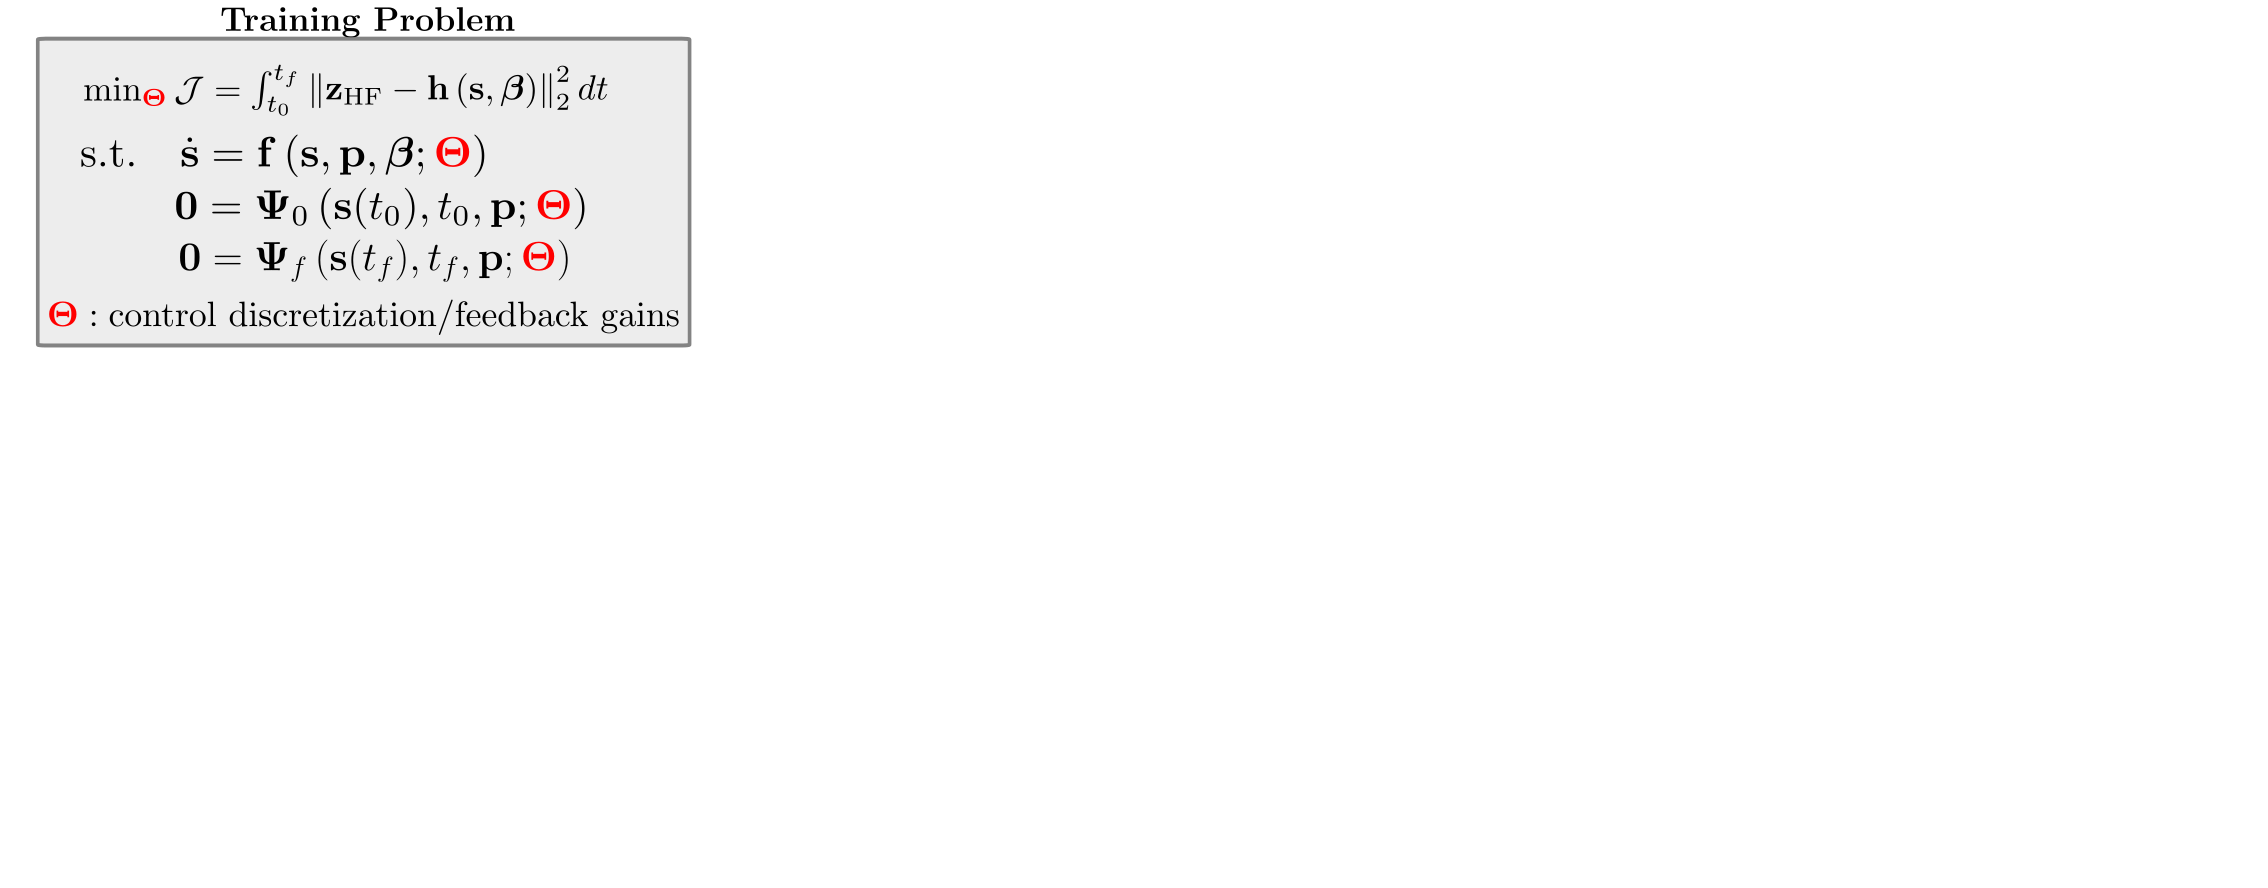
\includegraphics[width=0.95\textwidth]{../figs/ct/ct_overview_1.png}
        \end{figure}}
    \only<3>{
        \begin{figure}
            \centering
            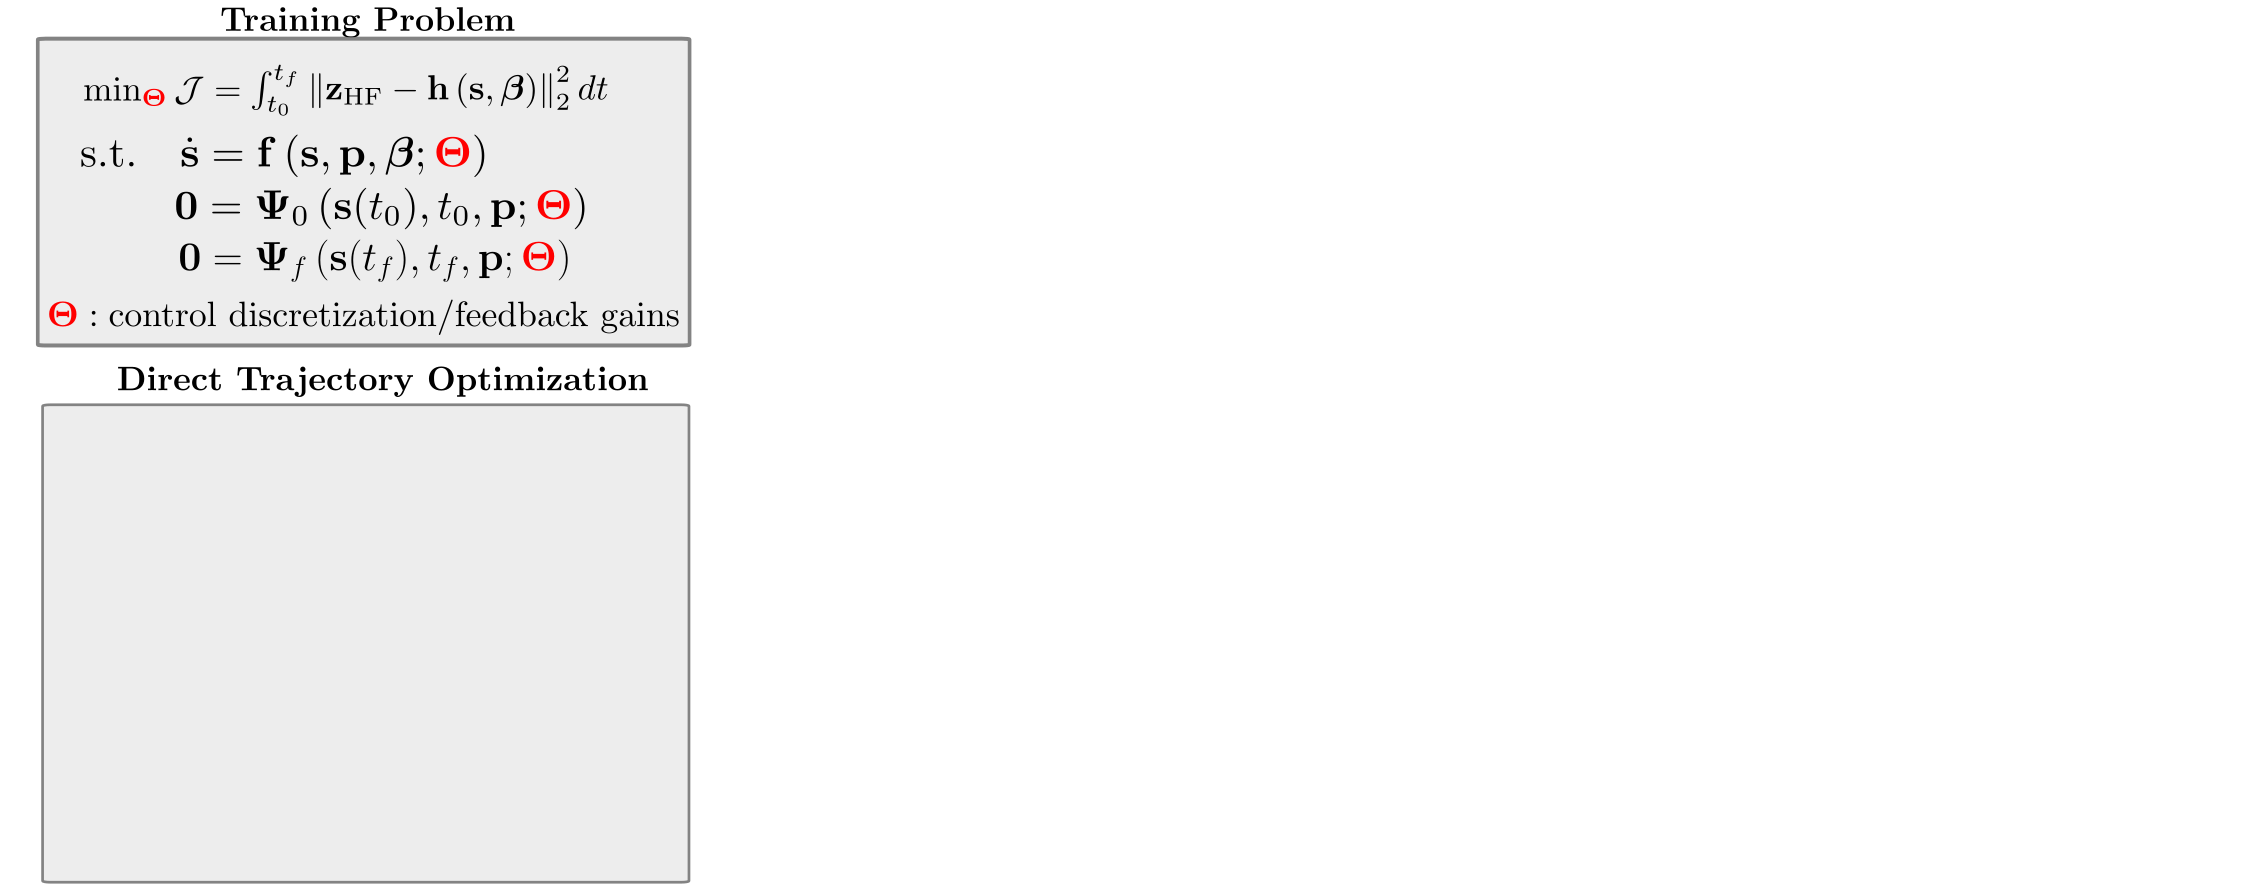
\includegraphics[width=0.95\textwidth]{../figs/ct/ct_overview_2.png}
        \end{figure}}
    \only<4>{
        \begin{figure}
            \centering
            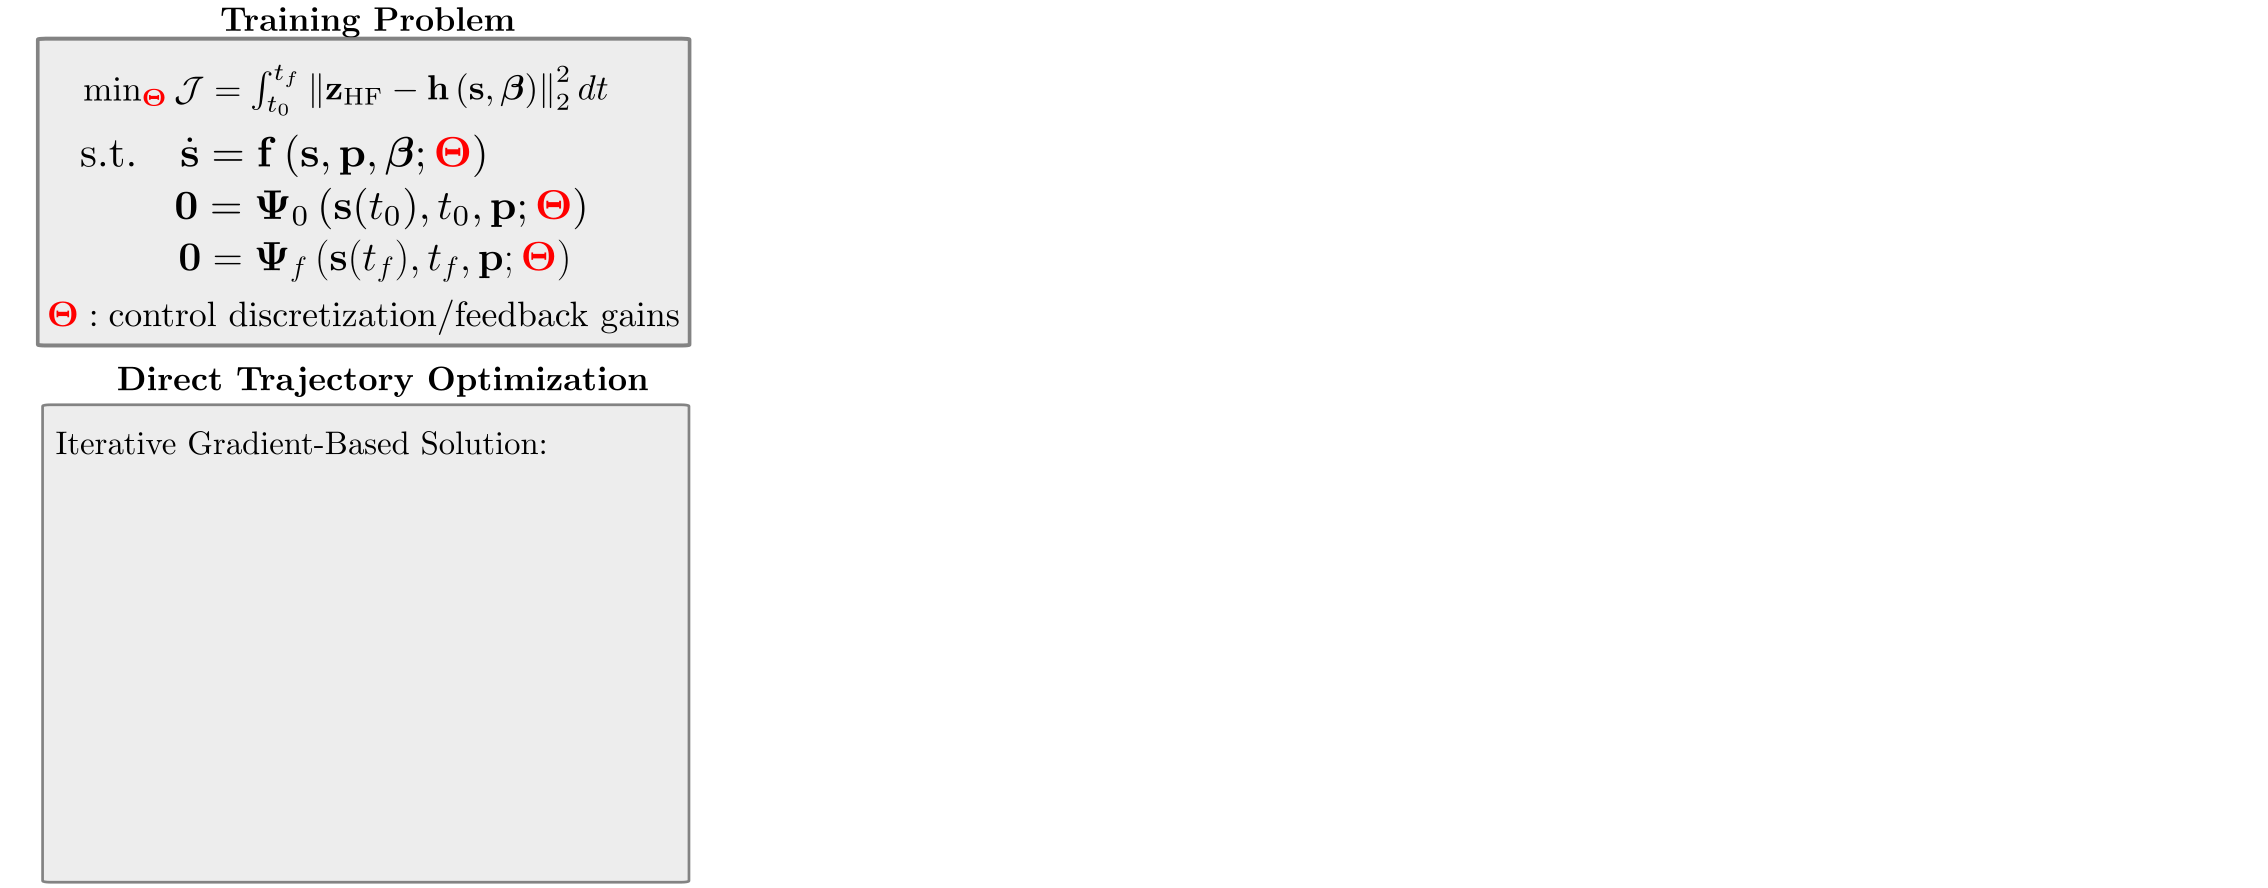
\includegraphics[width=0.95\textwidth]{../figs/ct/ct_overview_3.png}
        \end{figure}}
    \only<5>{
        \begin{figure}
            \centering
            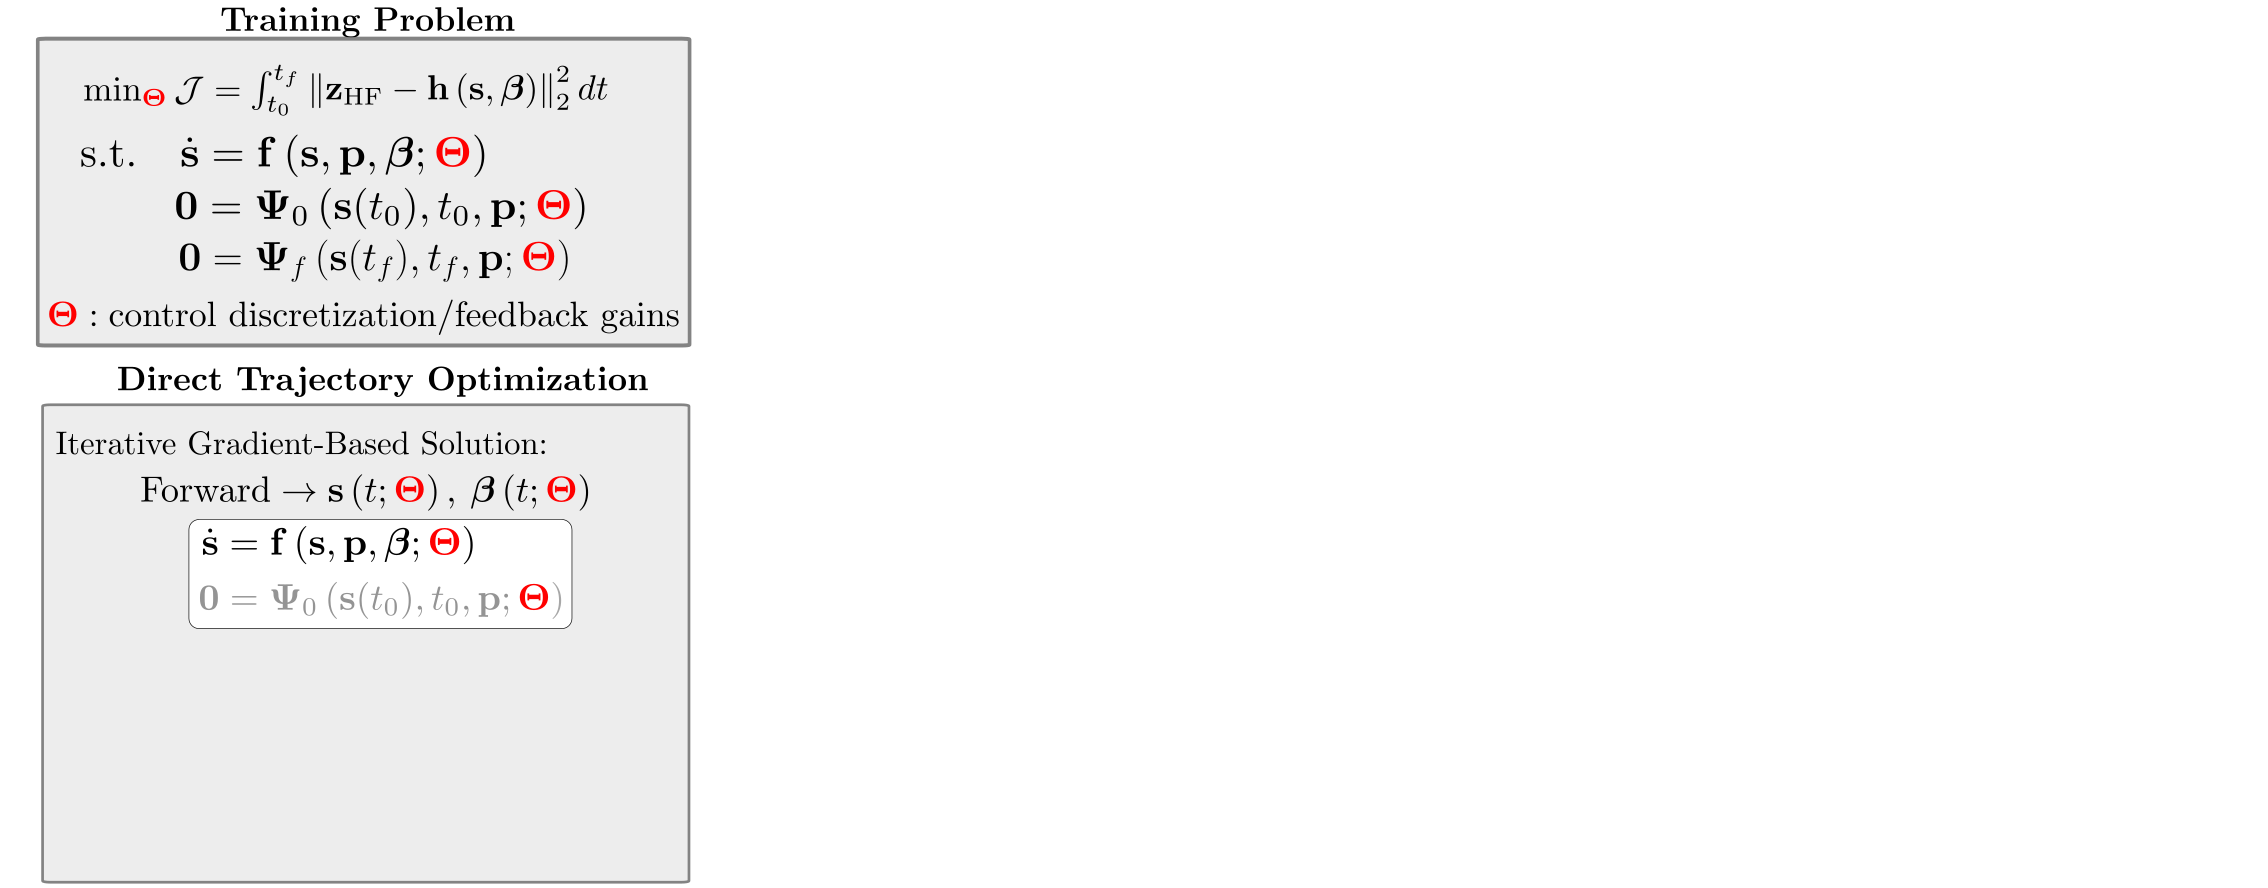
\includegraphics[width=0.95\textwidth]{../figs/ct/ct_overview_4.png}
        \end{figure}}
    \only<6>{
        \begin{figure}
            \centering
            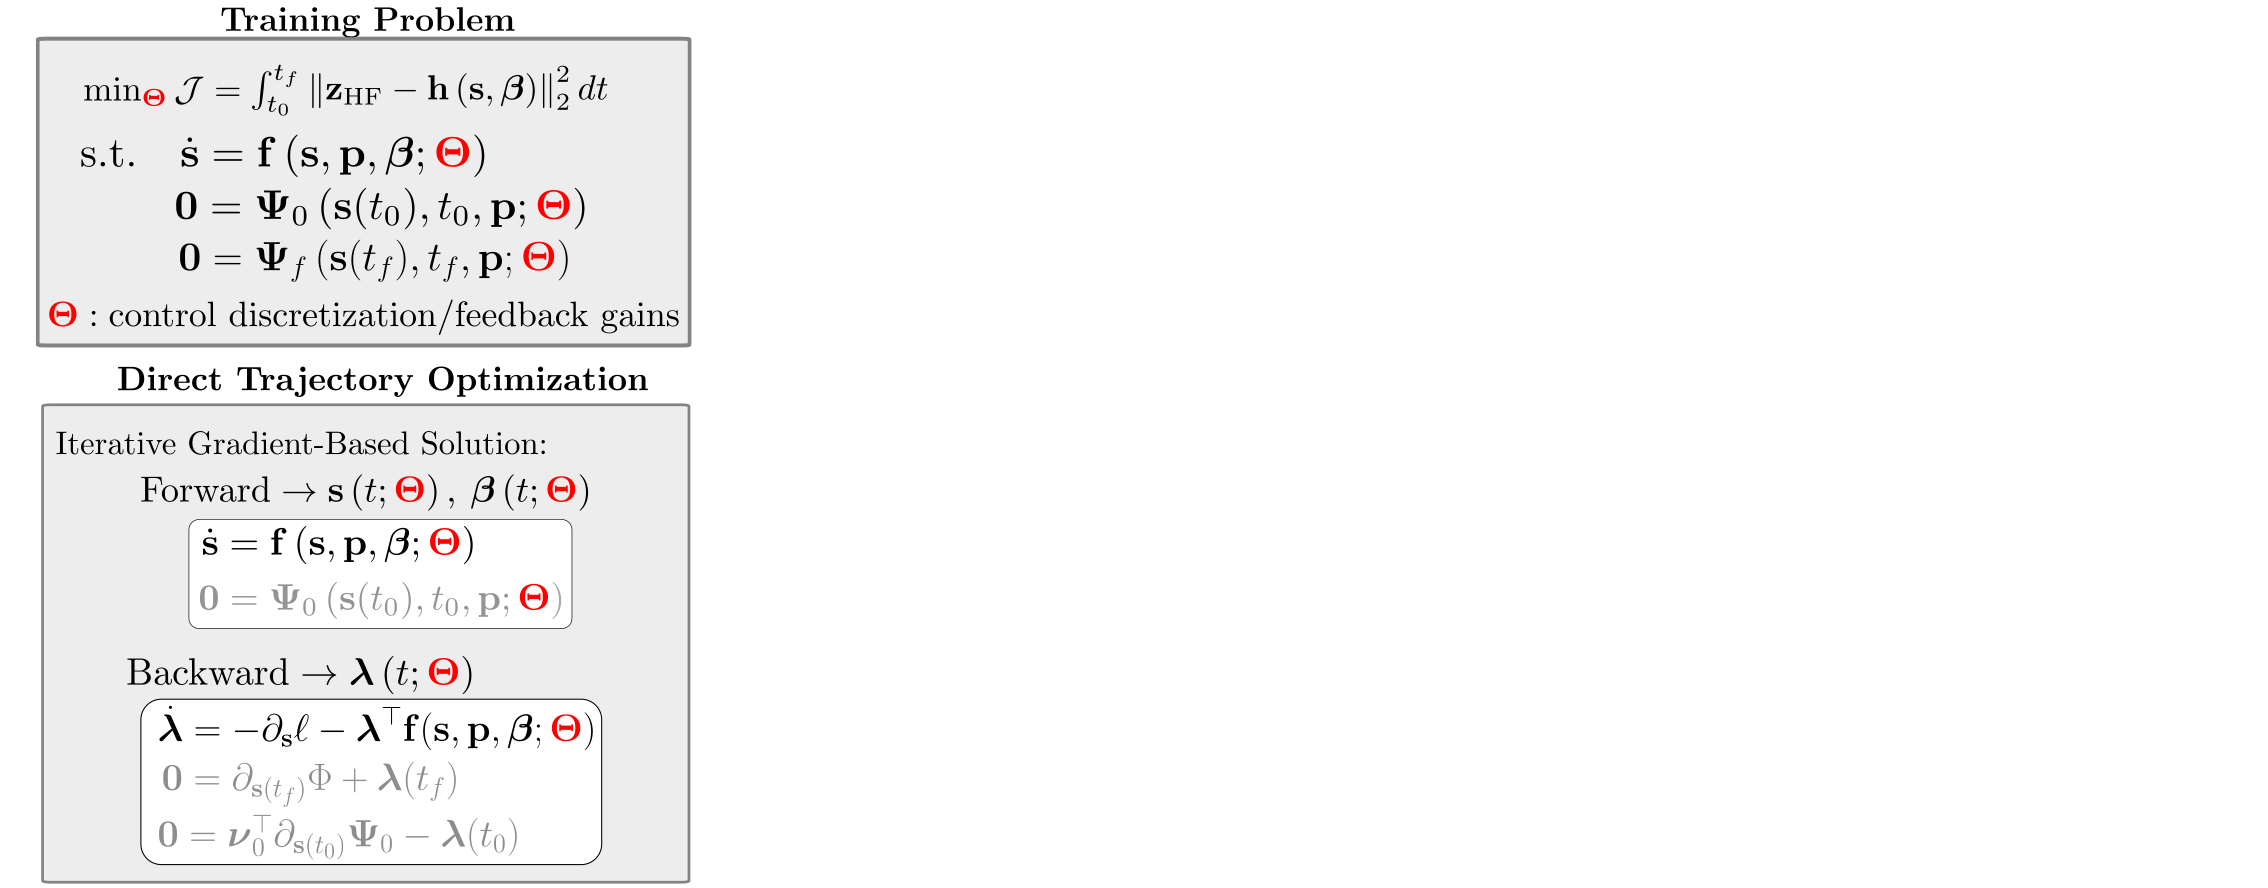
\includegraphics[width=0.95\textwidth]{../figs/ct/ct_overview_5.png}
        \end{figure}}
    \only<7>{
        \begin{figure}
            \centering
            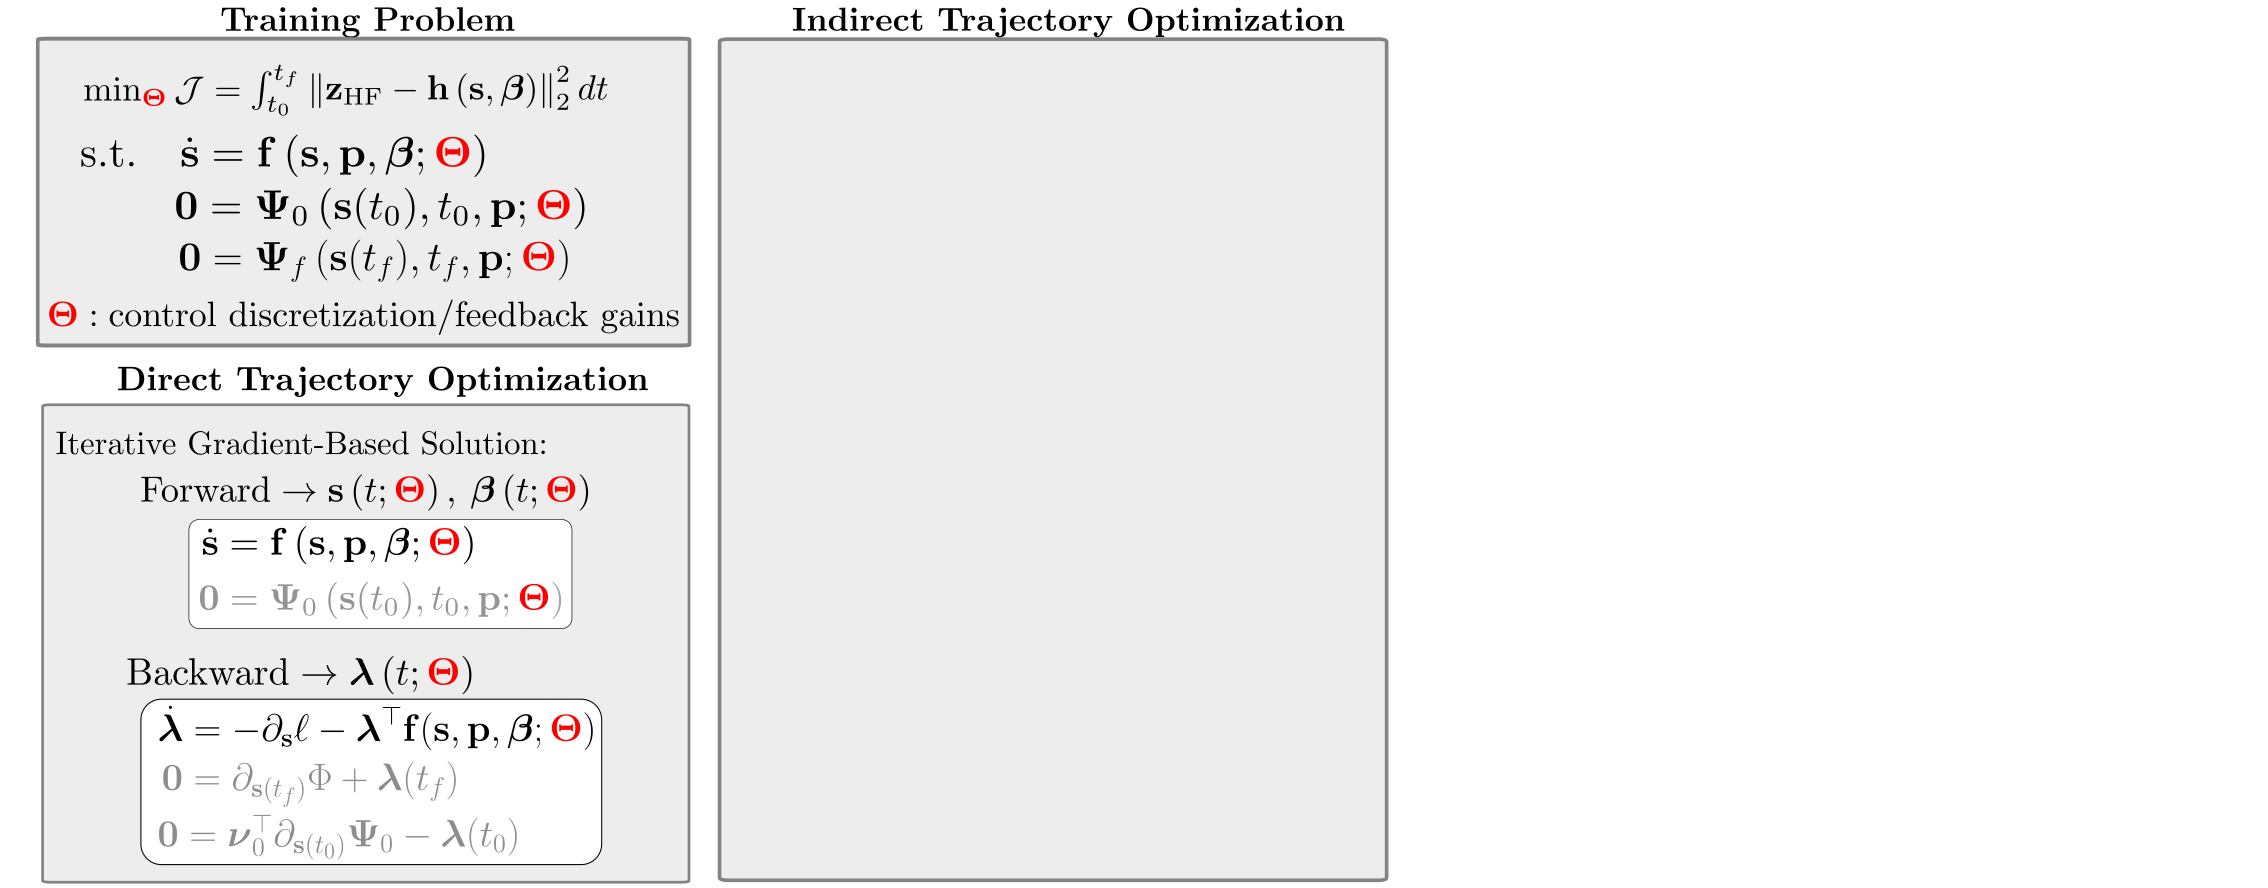
\includegraphics[width=0.95\textwidth]{../figs/ct/ct_overview_6.png}
        \end{figure}}
    \only<8>{
        \begin{figure}
            \centering
            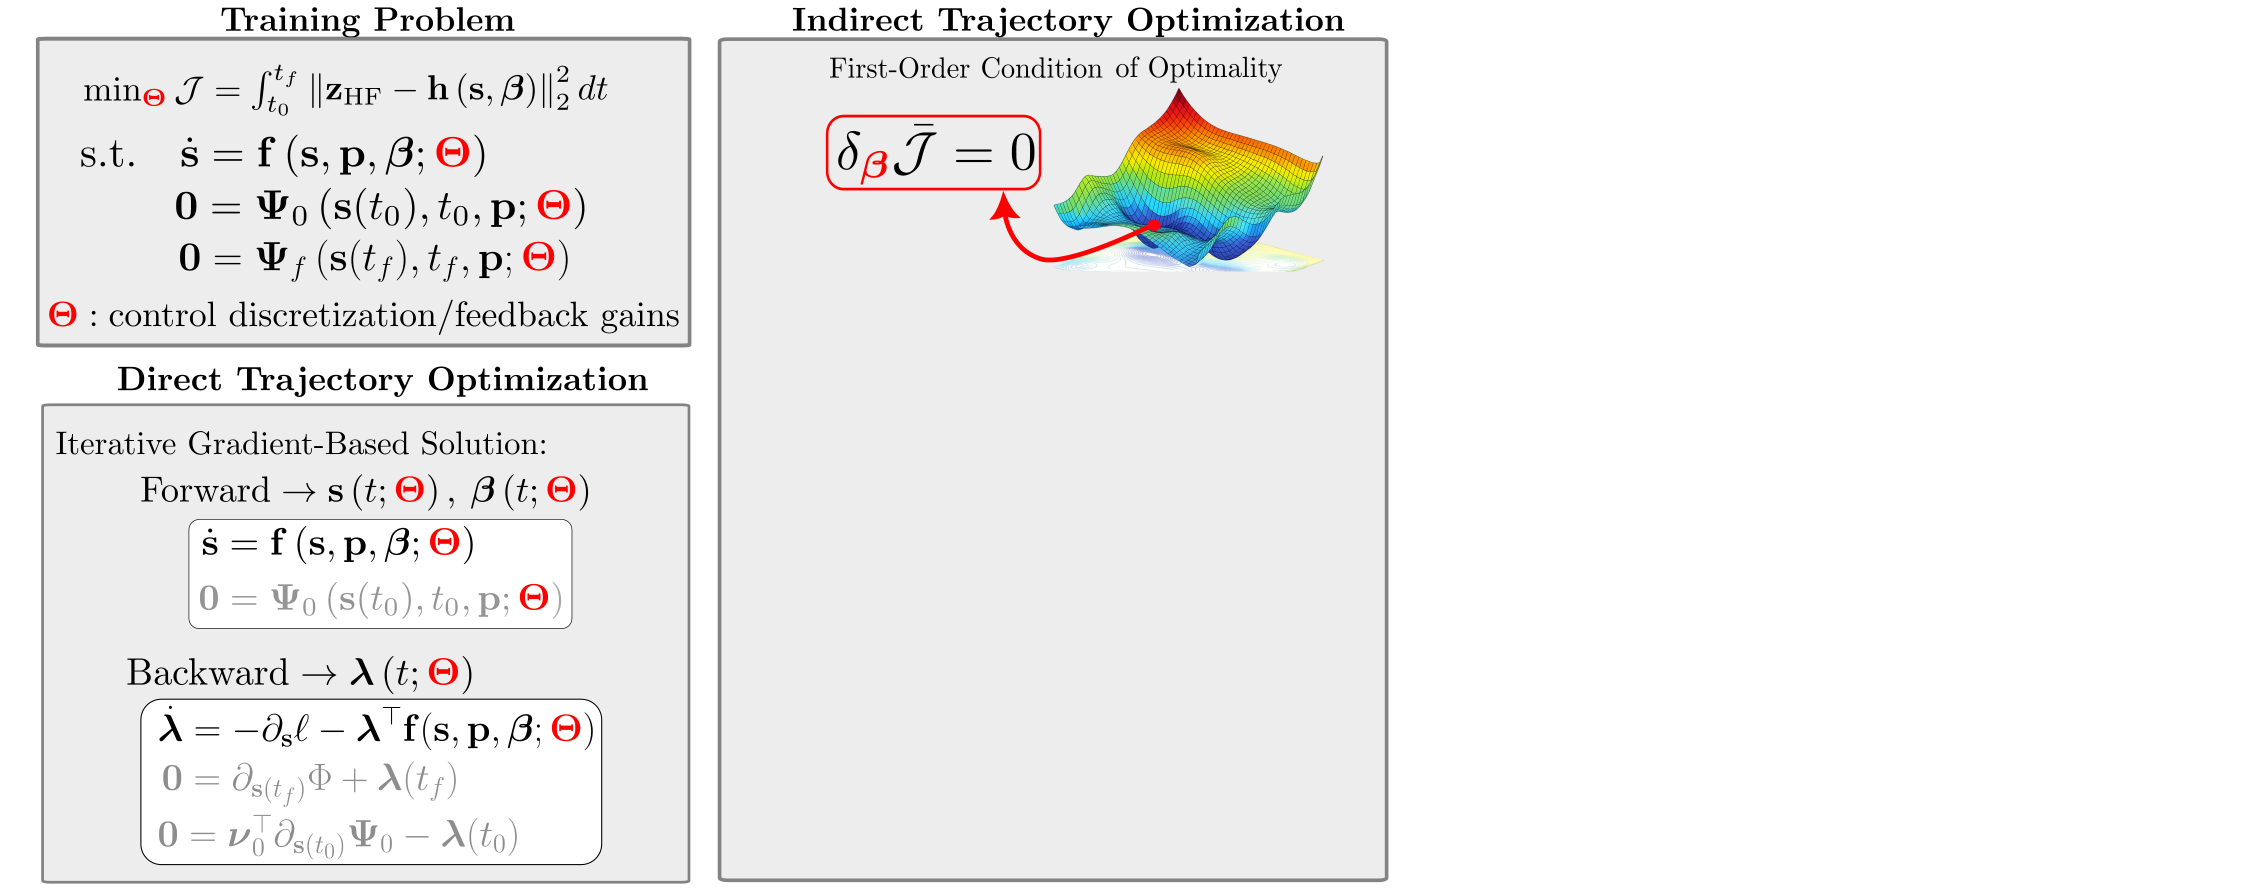
\includegraphics[width=0.95\textwidth]{../figs/ct/ct_overview_7.png}
        \end{figure}}
    \only<9>{
        \begin{figure}
            \centering
            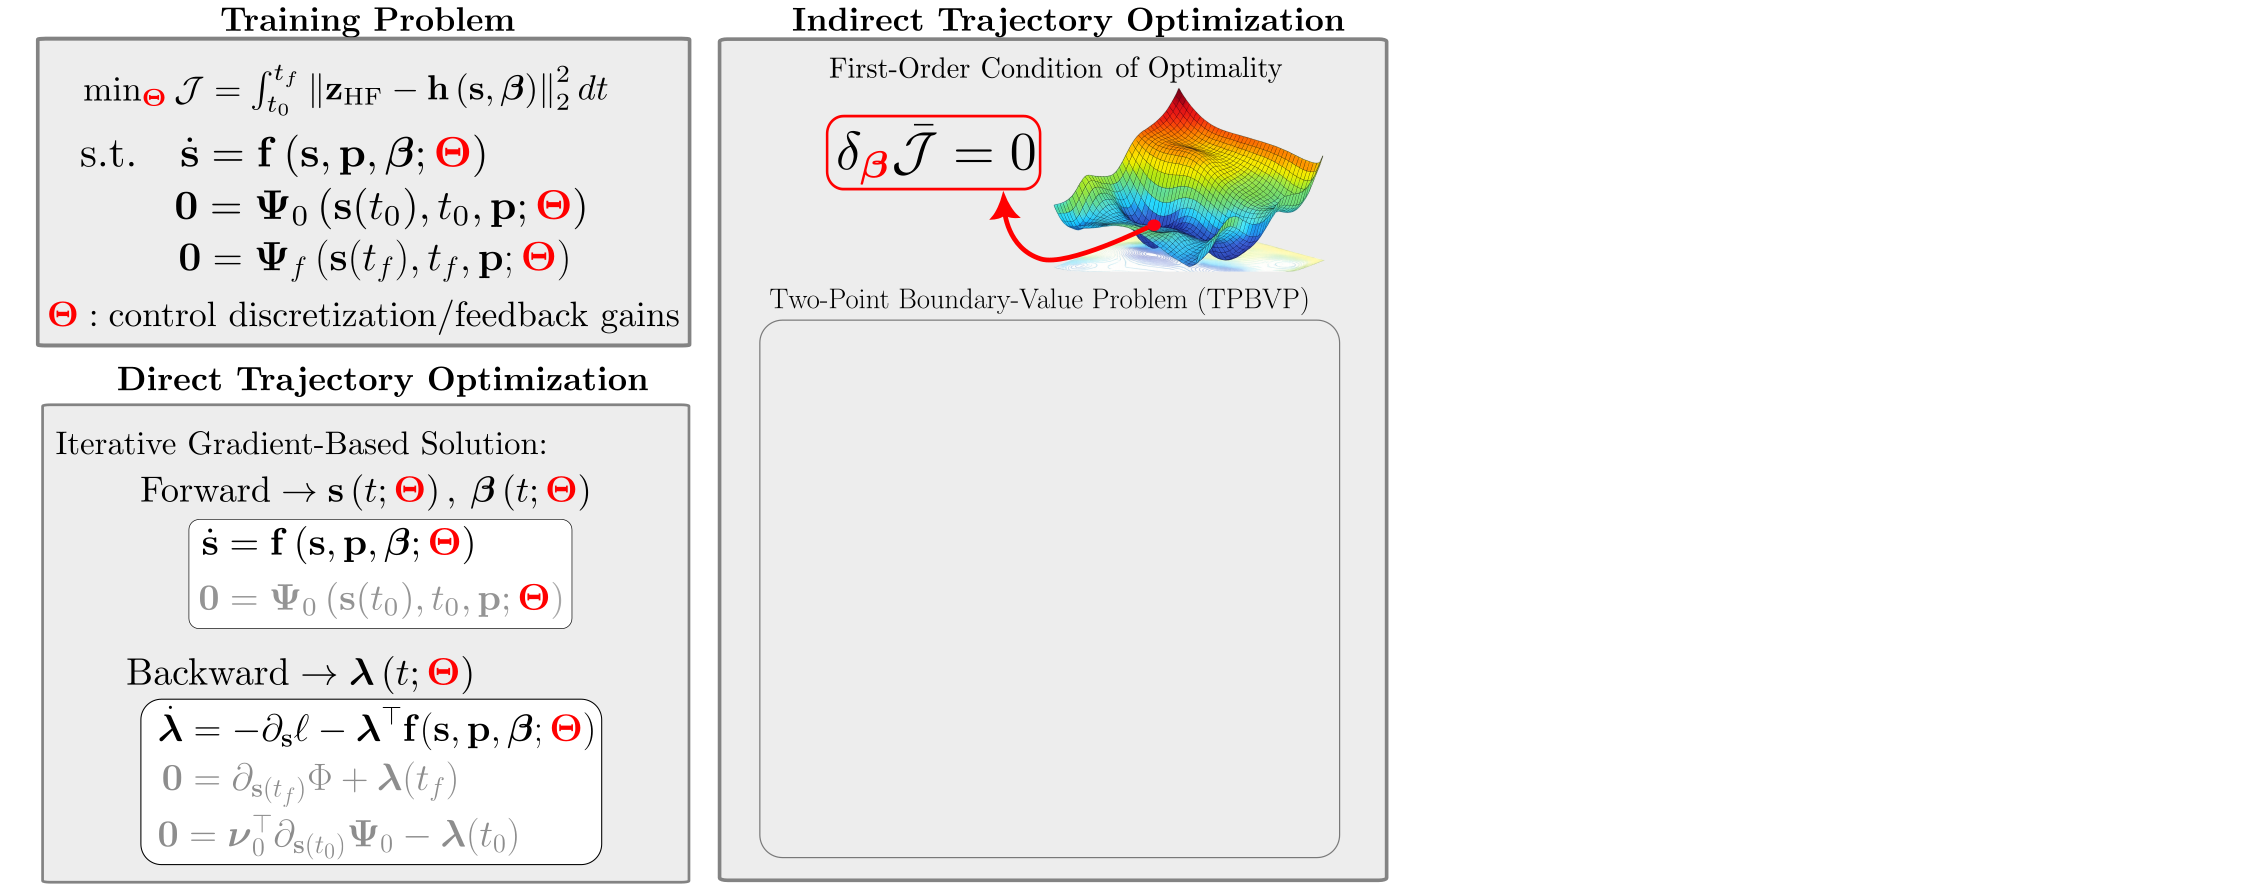
\includegraphics[width=0.95\textwidth]{../figs/ct/ct_overview_8.png}
        \end{figure}}
    \only<10>{
        \begin{figure}
            \centering
            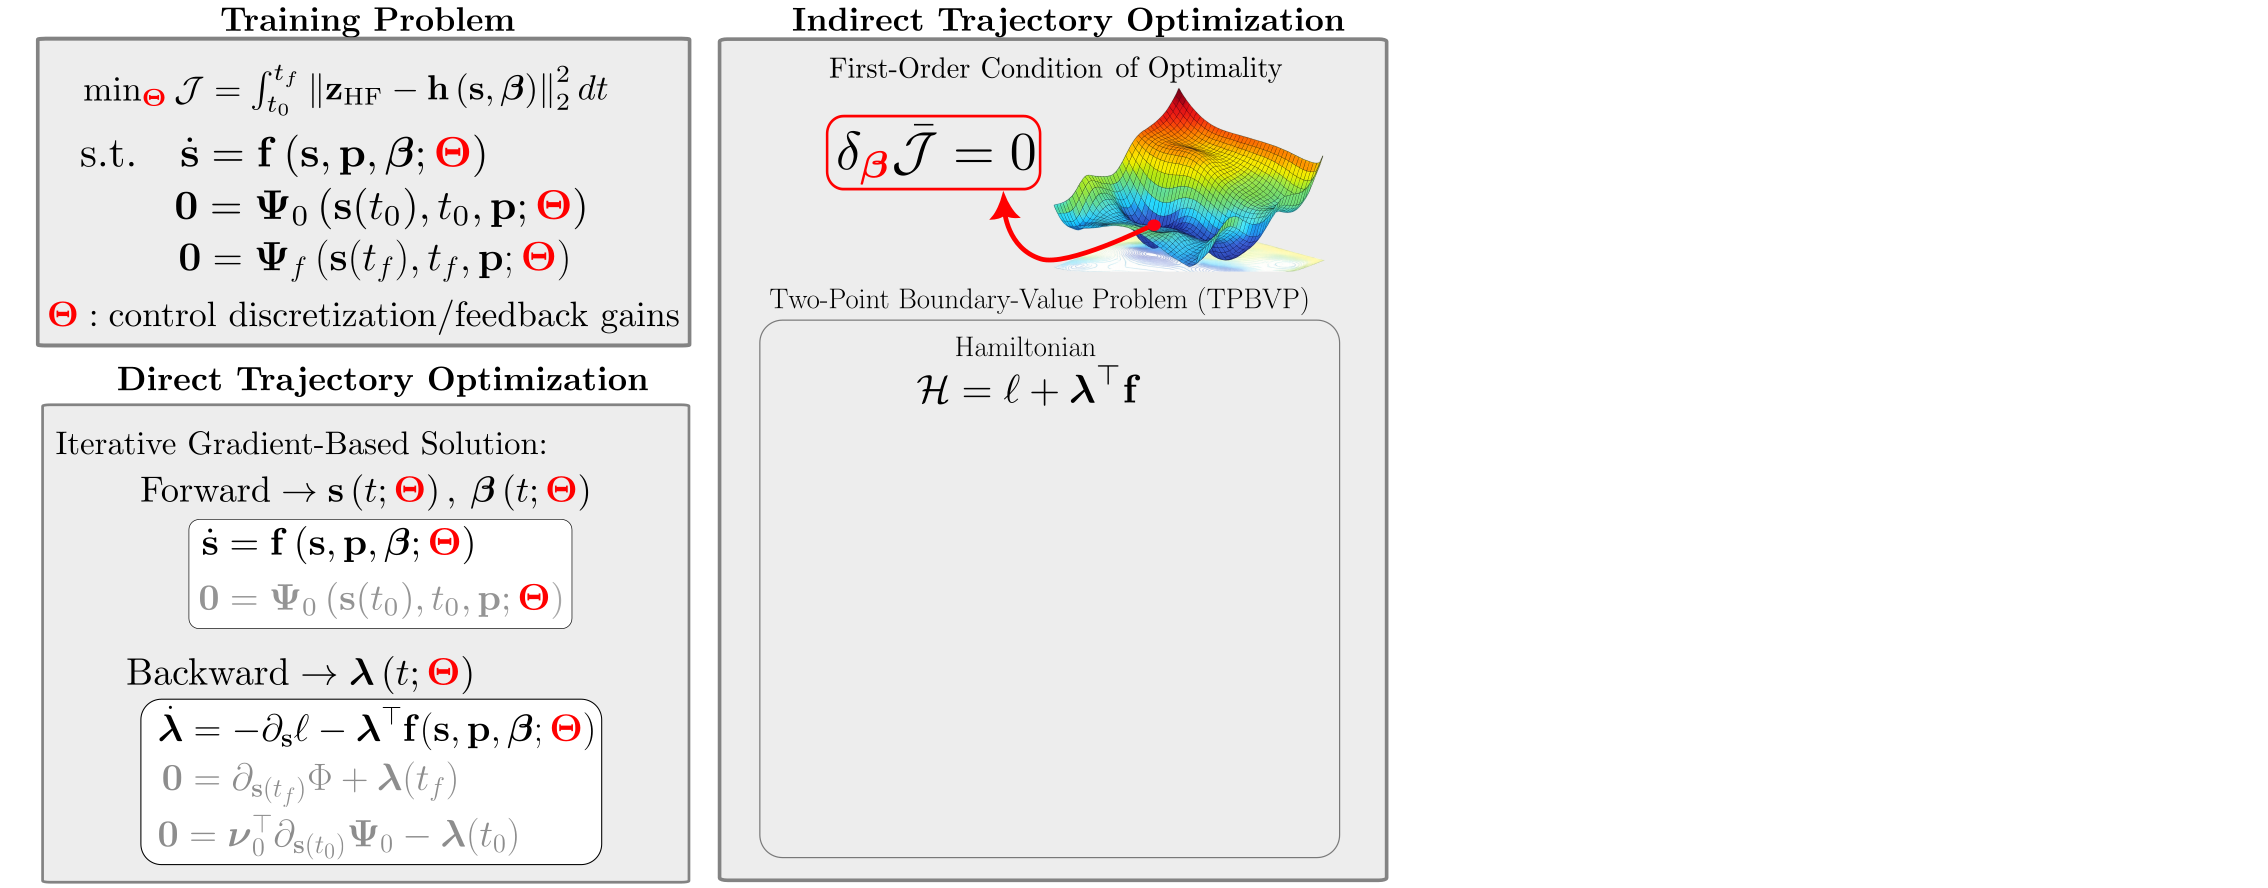
\includegraphics[width=0.95\textwidth]{../figs/ct/ct_overview_9.png}
        \end{figure}}
    \only<11>{
        \begin{figure}
            \centering
            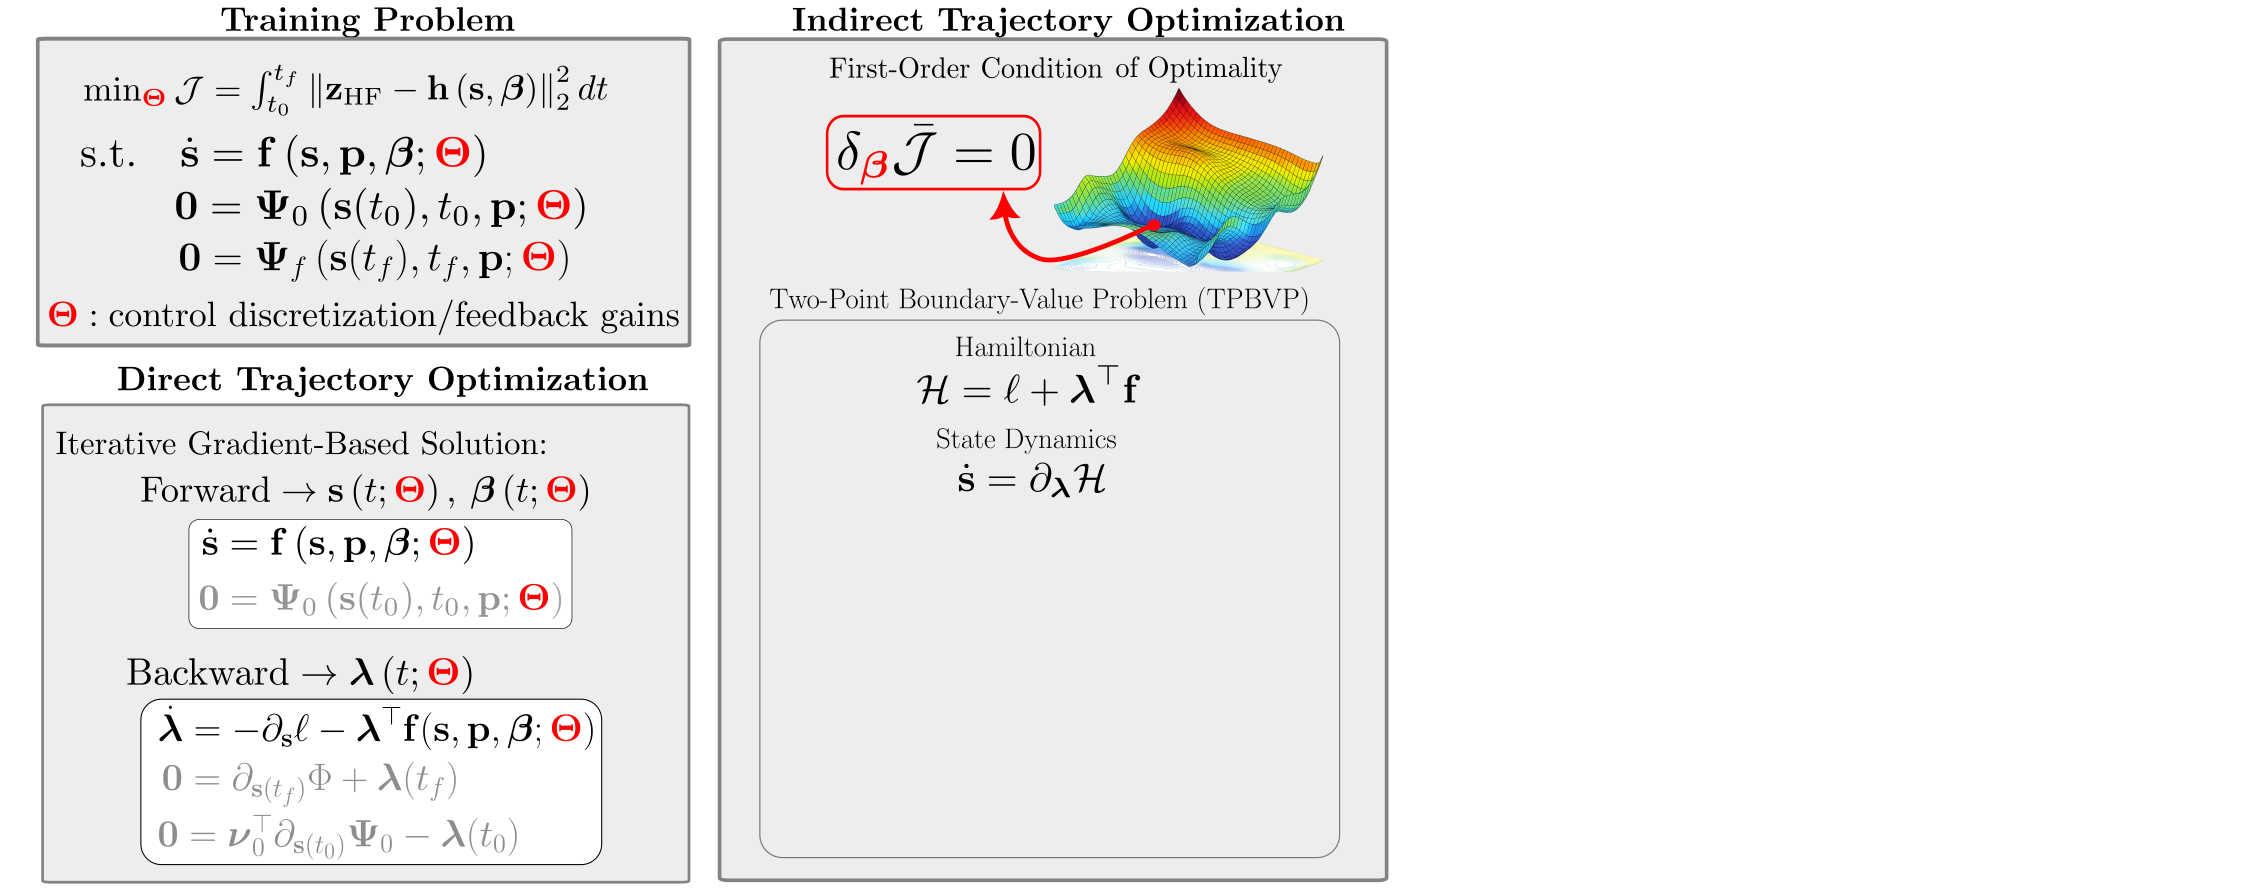
\includegraphics[width=0.95\textwidth]{../figs/ct/ct_overview_10.png}
        \end{figure}}
    \only<12>{
        \begin{figure}
            \centering
            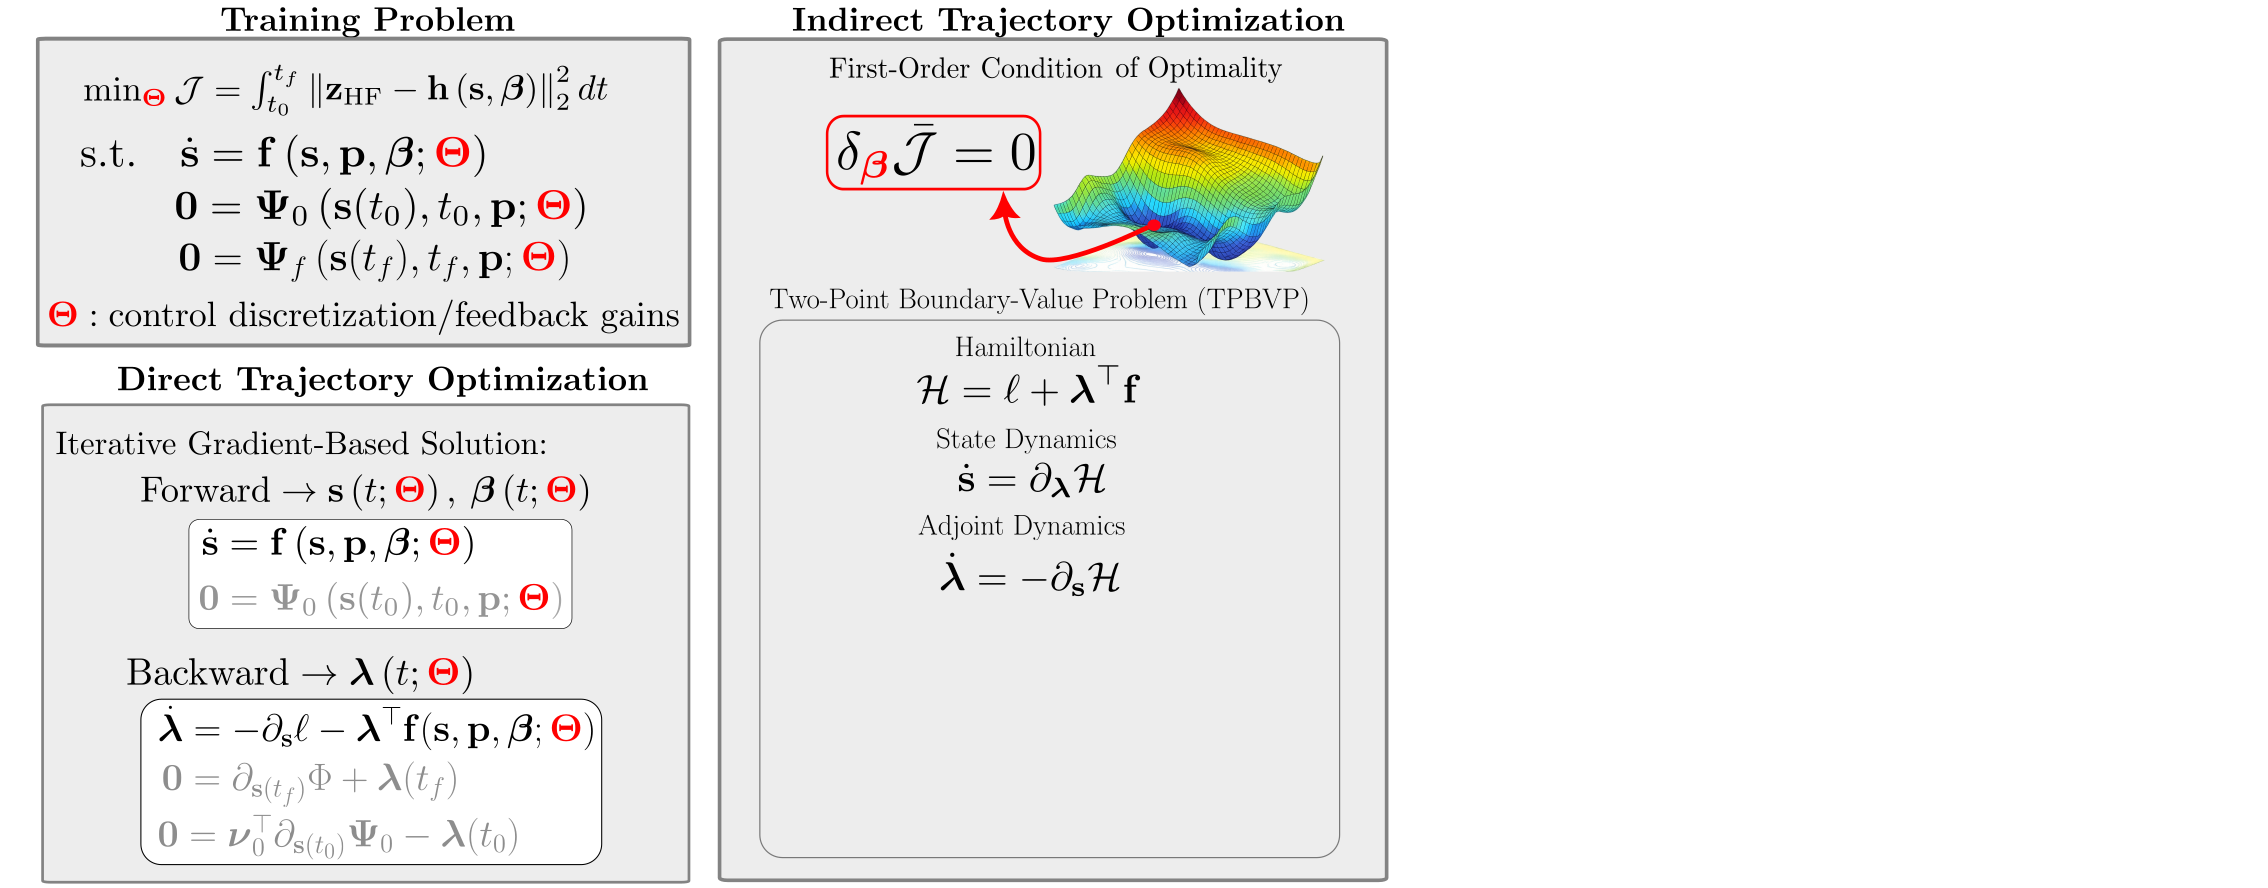
\includegraphics[width=0.95\textwidth]{../figs/ct/ct_overview_11.png}
        \end{figure}}
    \only<13>{
        \begin{figure}
            \centering
            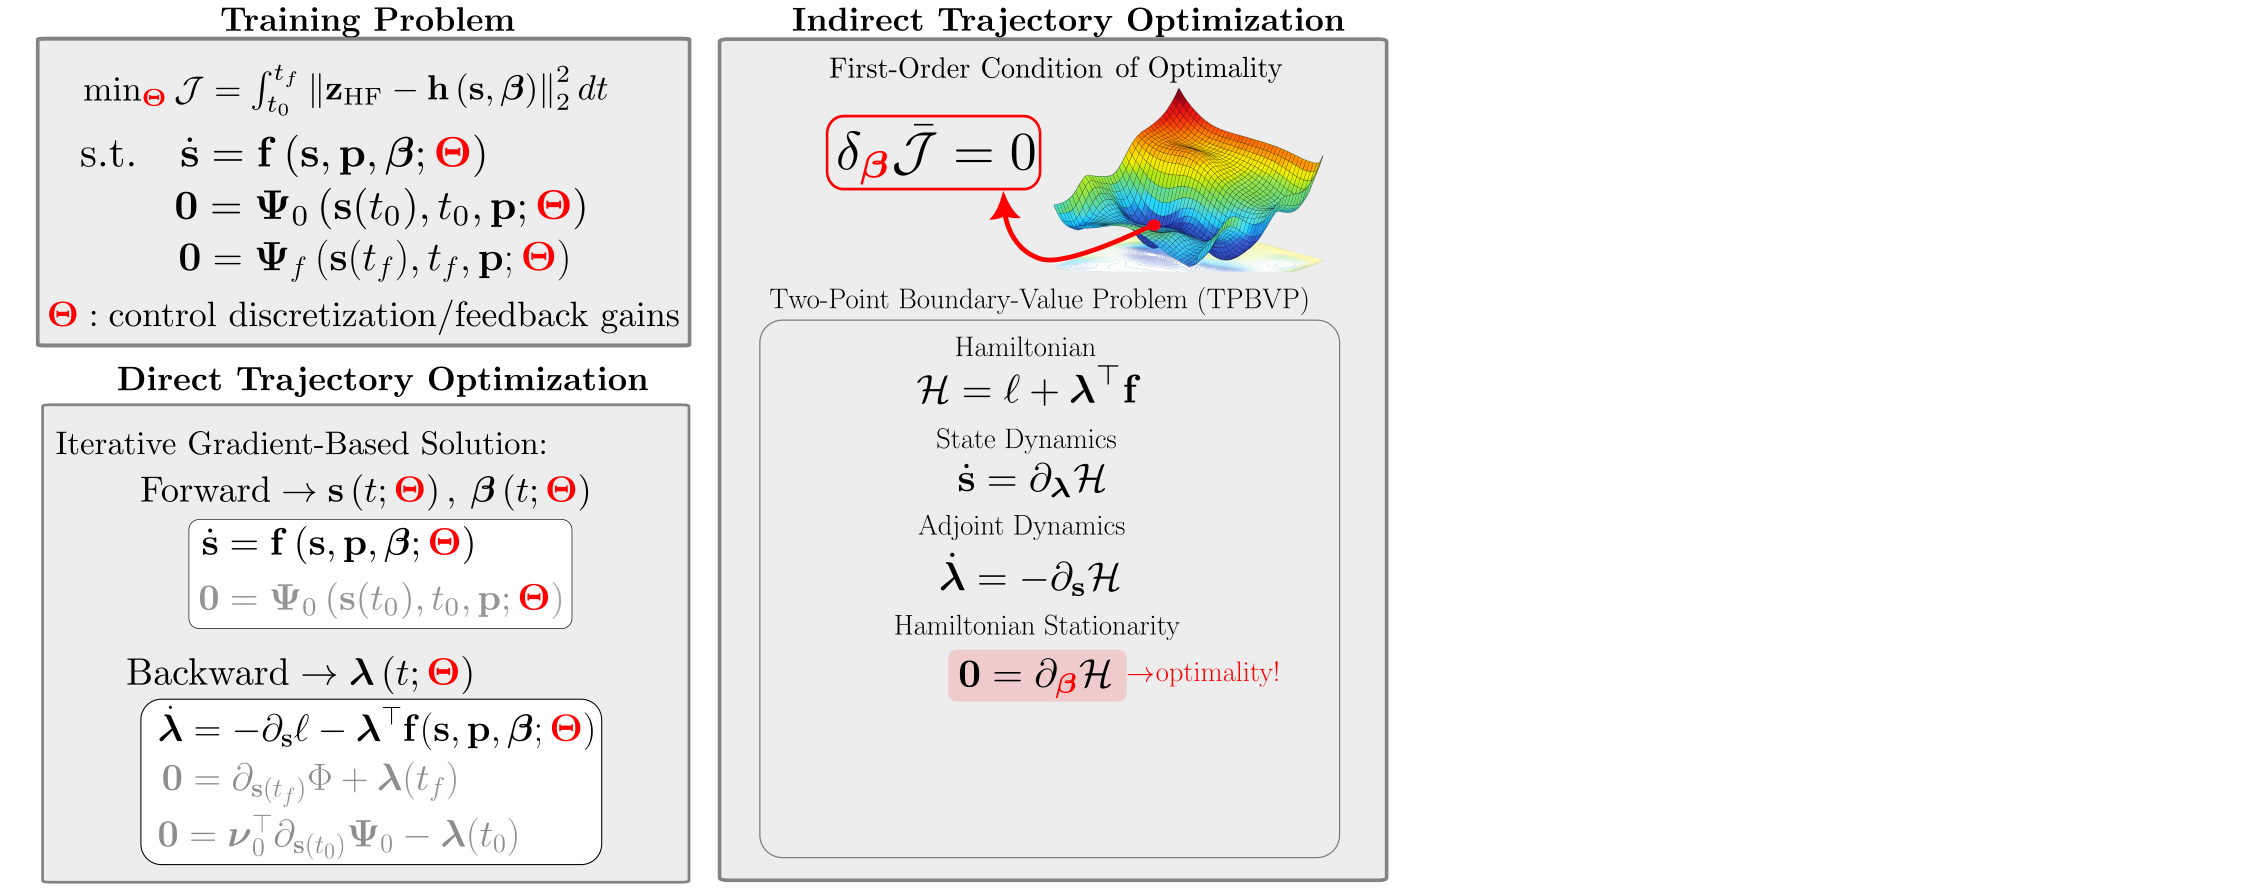
\includegraphics[width=0.95\textwidth]{../figs/ct/ct_overview_12.png}
        \end{figure}}
    \only<14>{
        \begin{figure}
            \centering
            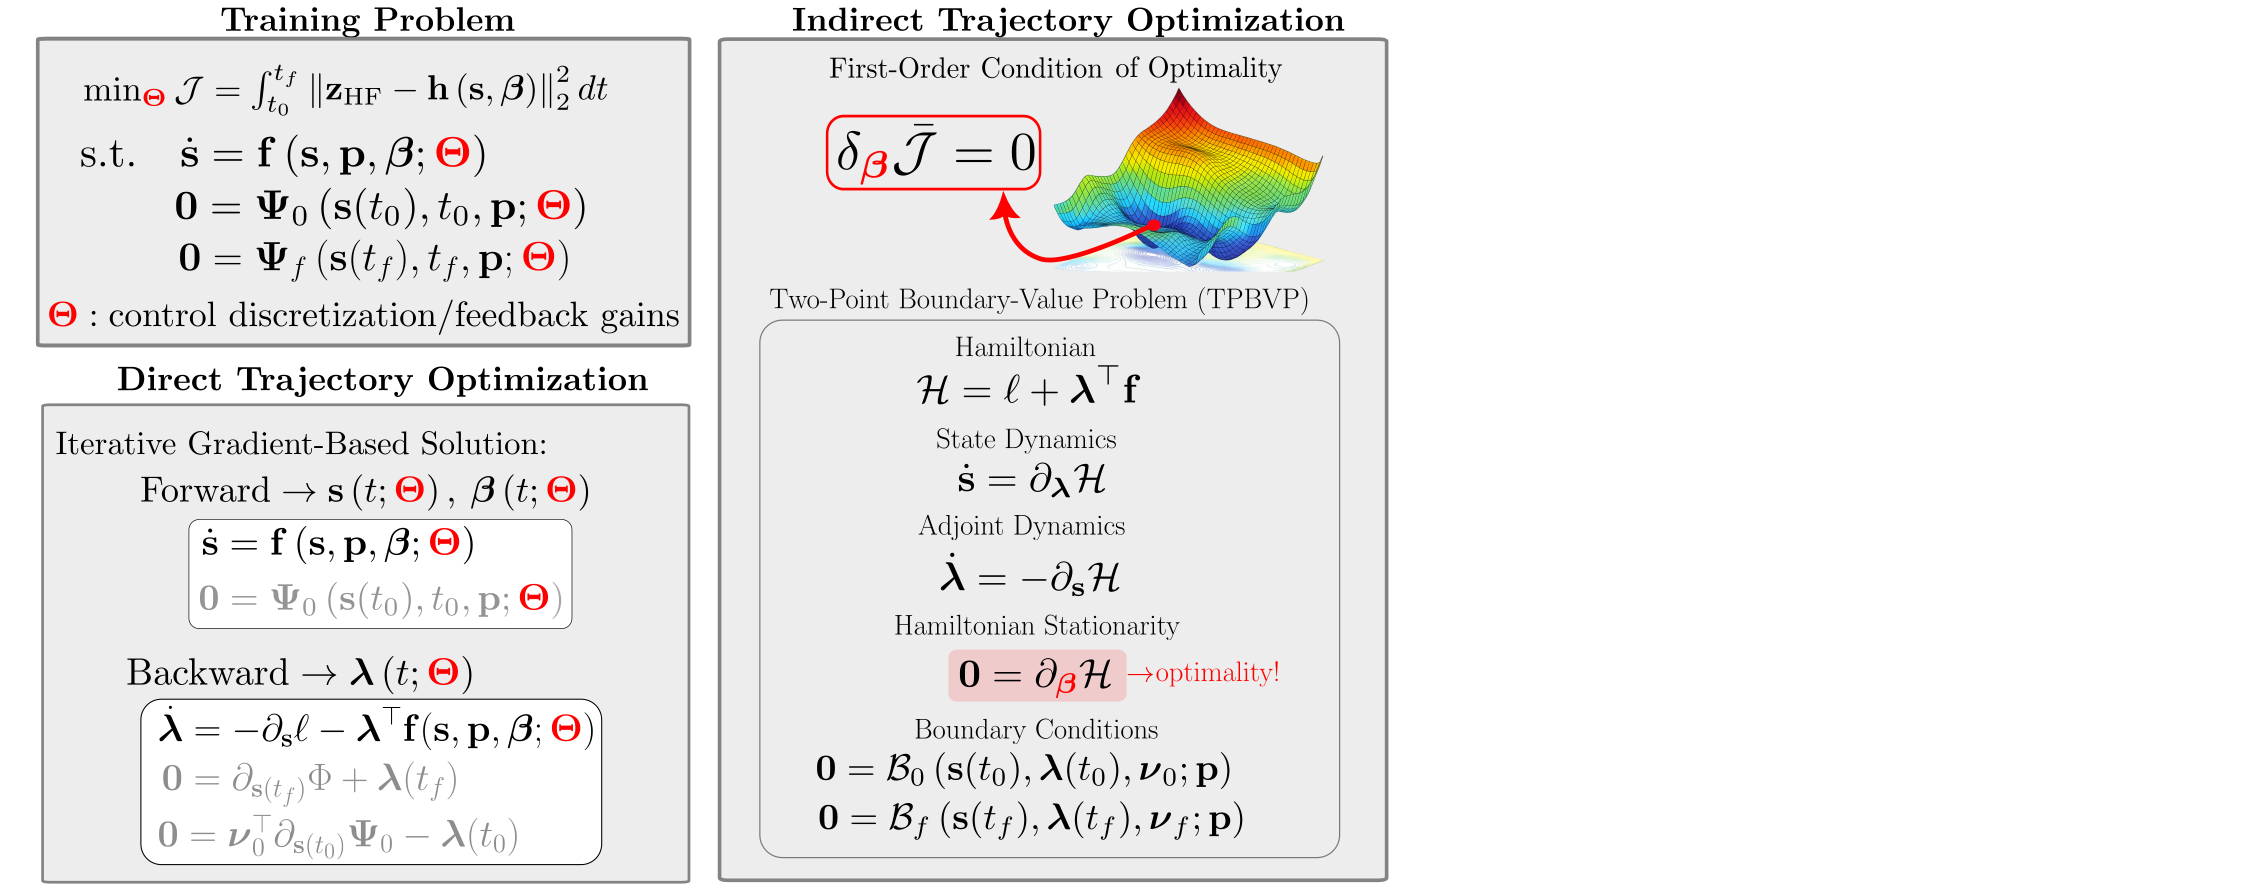
\includegraphics[width=0.95\textwidth]{../figs/ct/ct_overview_13.png}
        \end{figure}}
    \only<15>{
        \begin{figure}
            \centering
            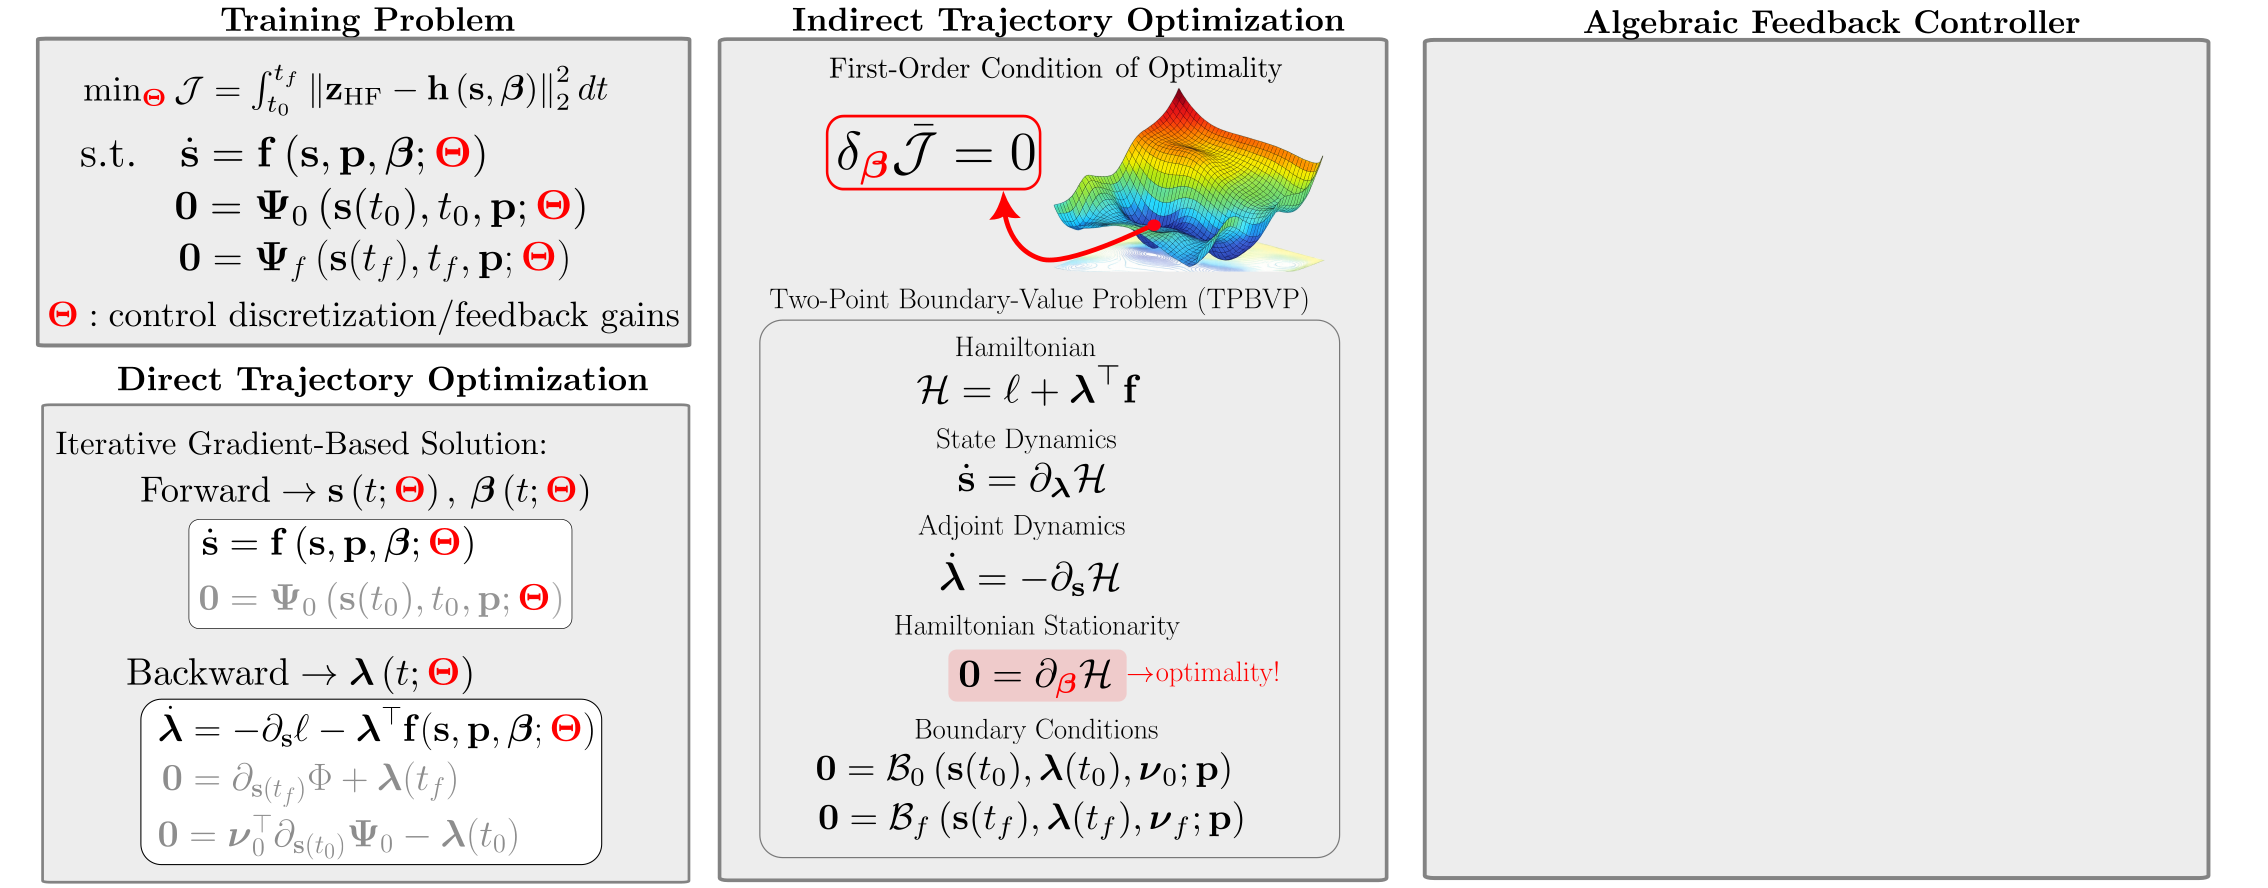
\includegraphics[width=0.95\textwidth]{../figs/ct/ct_overview_14.png}
        \end{figure}}
    \only<16>{
        \begin{figure}
            \centering
            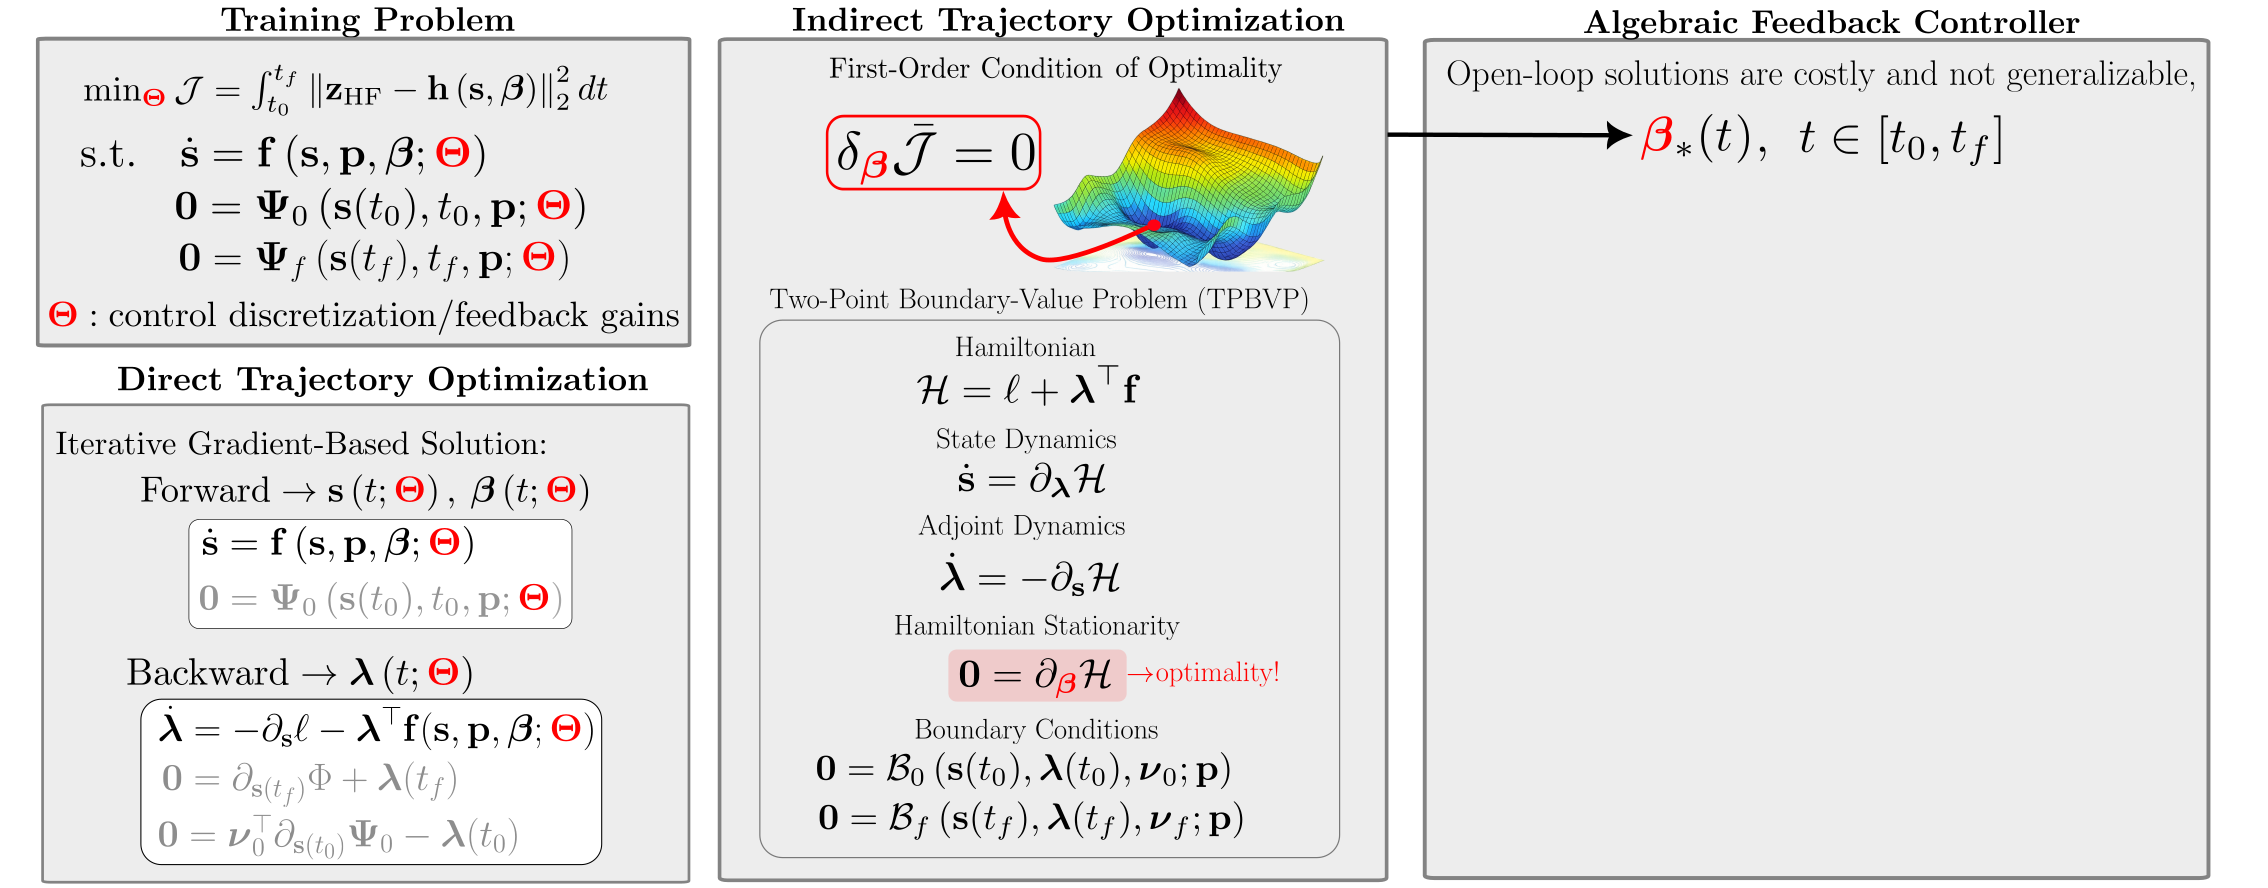
\includegraphics[width=0.95\textwidth]{../figs/ct/ct_overview_15.png}
        \end{figure}}
    \only<17>{
        \begin{figure}
            \centering
            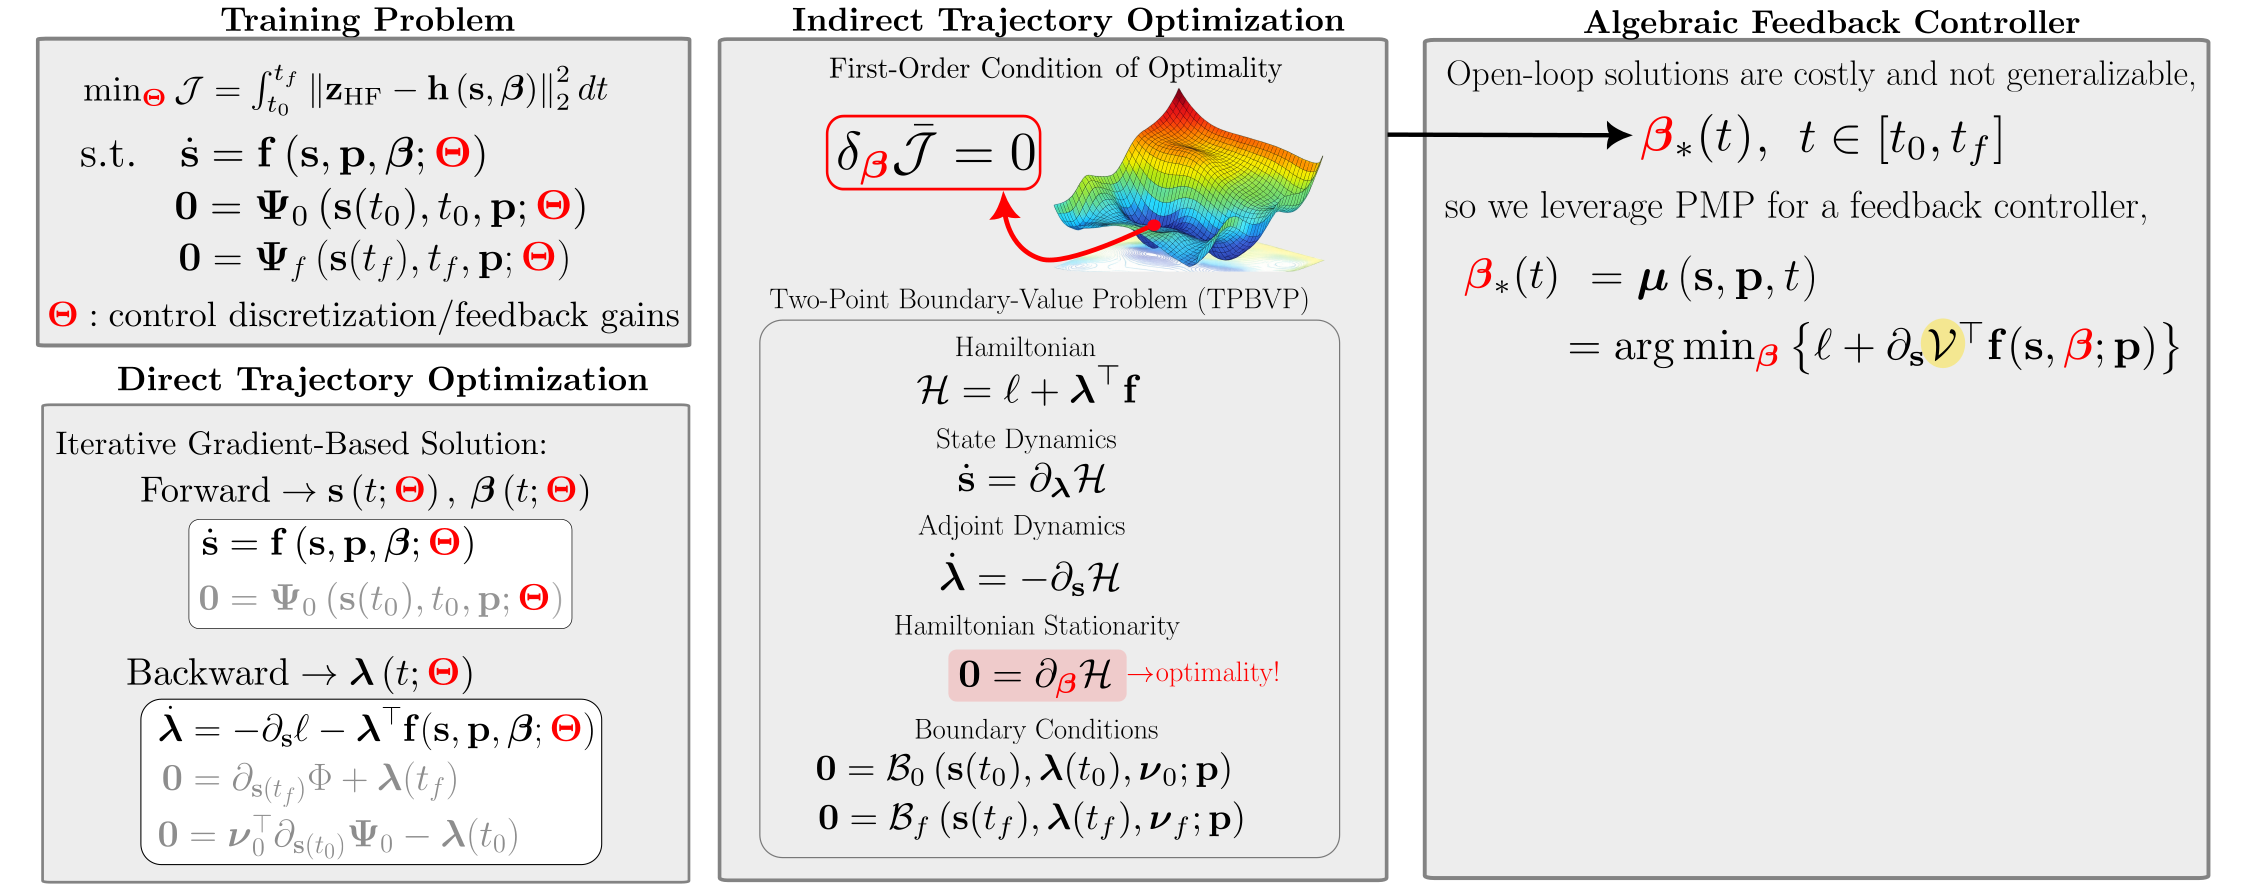
\includegraphics[width=0.95\textwidth]{../figs/ct/ct_overview_16.png}
        \end{figure}}
    \only<18>{
        \begin{figure}
            \centering
            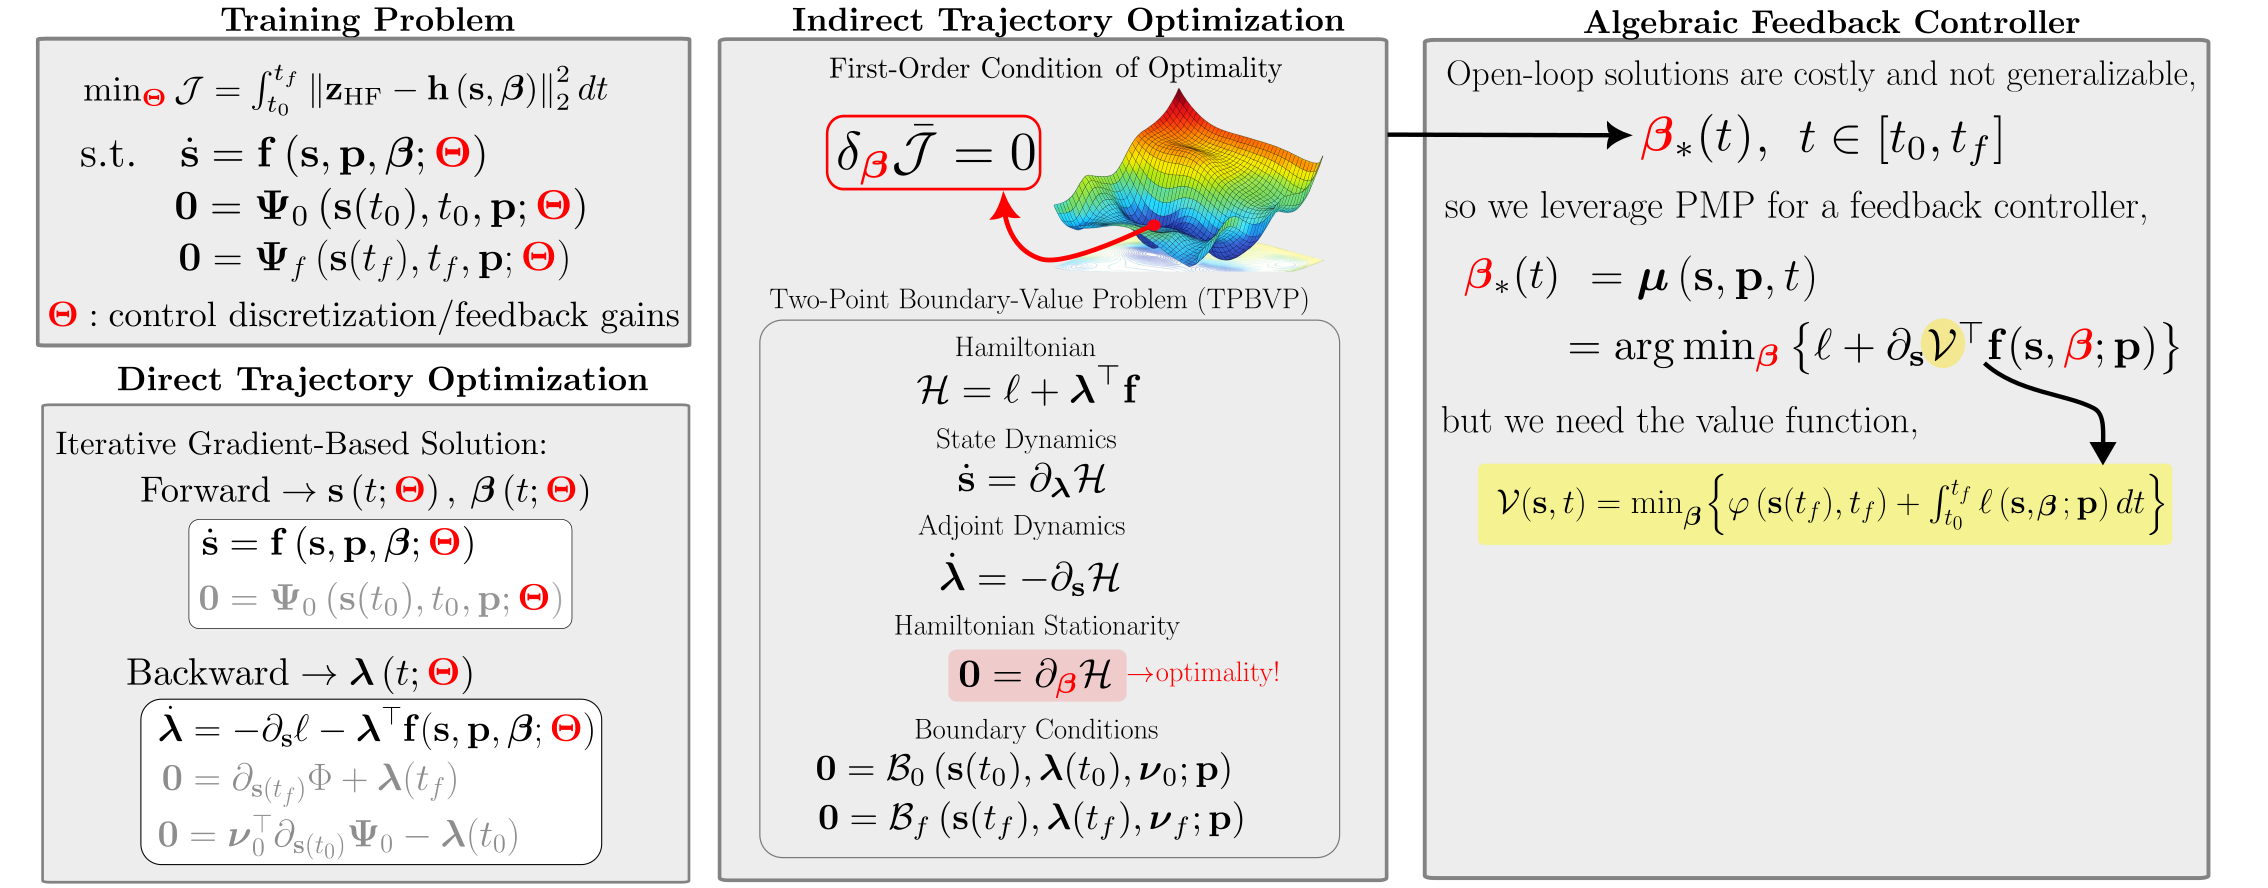
\includegraphics[width=0.95\textwidth]{../figs/ct/ct_overview_17.png}
        \end{figure}}
    \only<19>{
        \begin{figure}
            \centering
            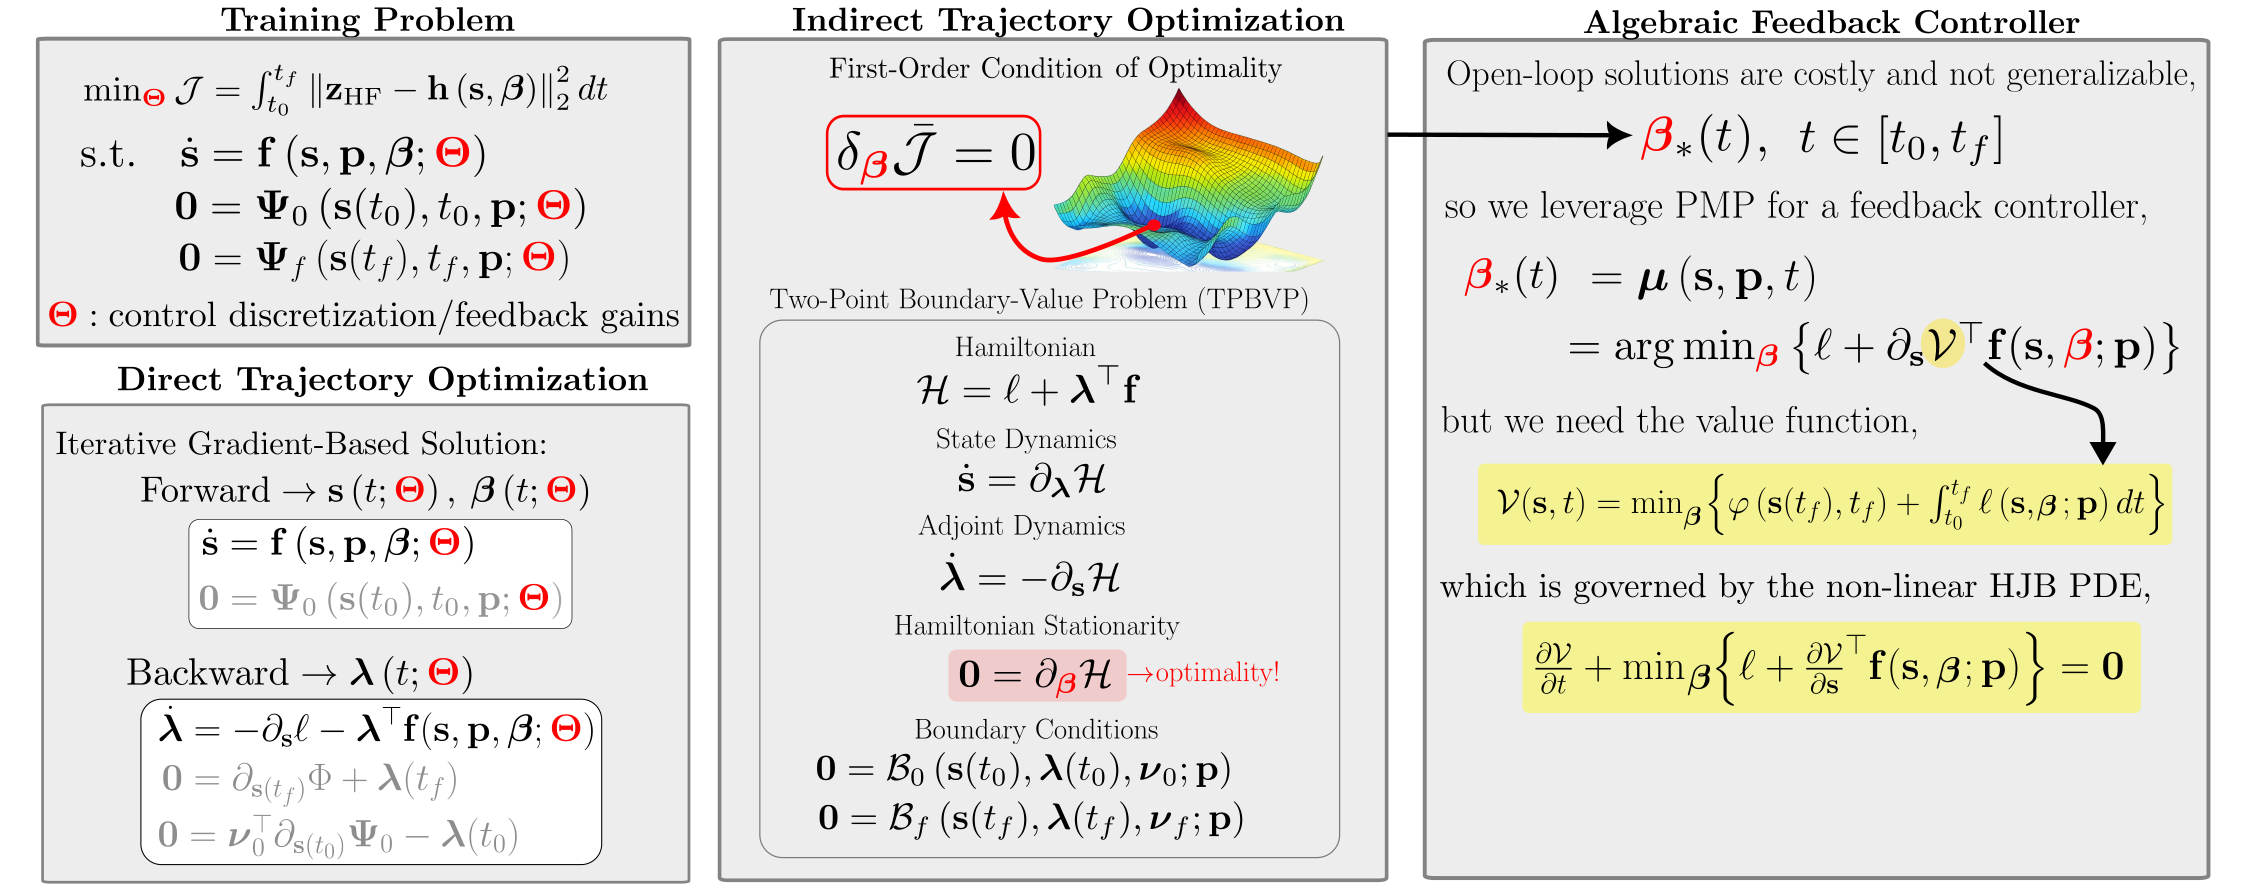
\includegraphics[width=0.95\textwidth]{../figs/ct/ct_overview_18.png}
        \end{figure}}
    \only<20>{
        \begin{figure}
            \centering
            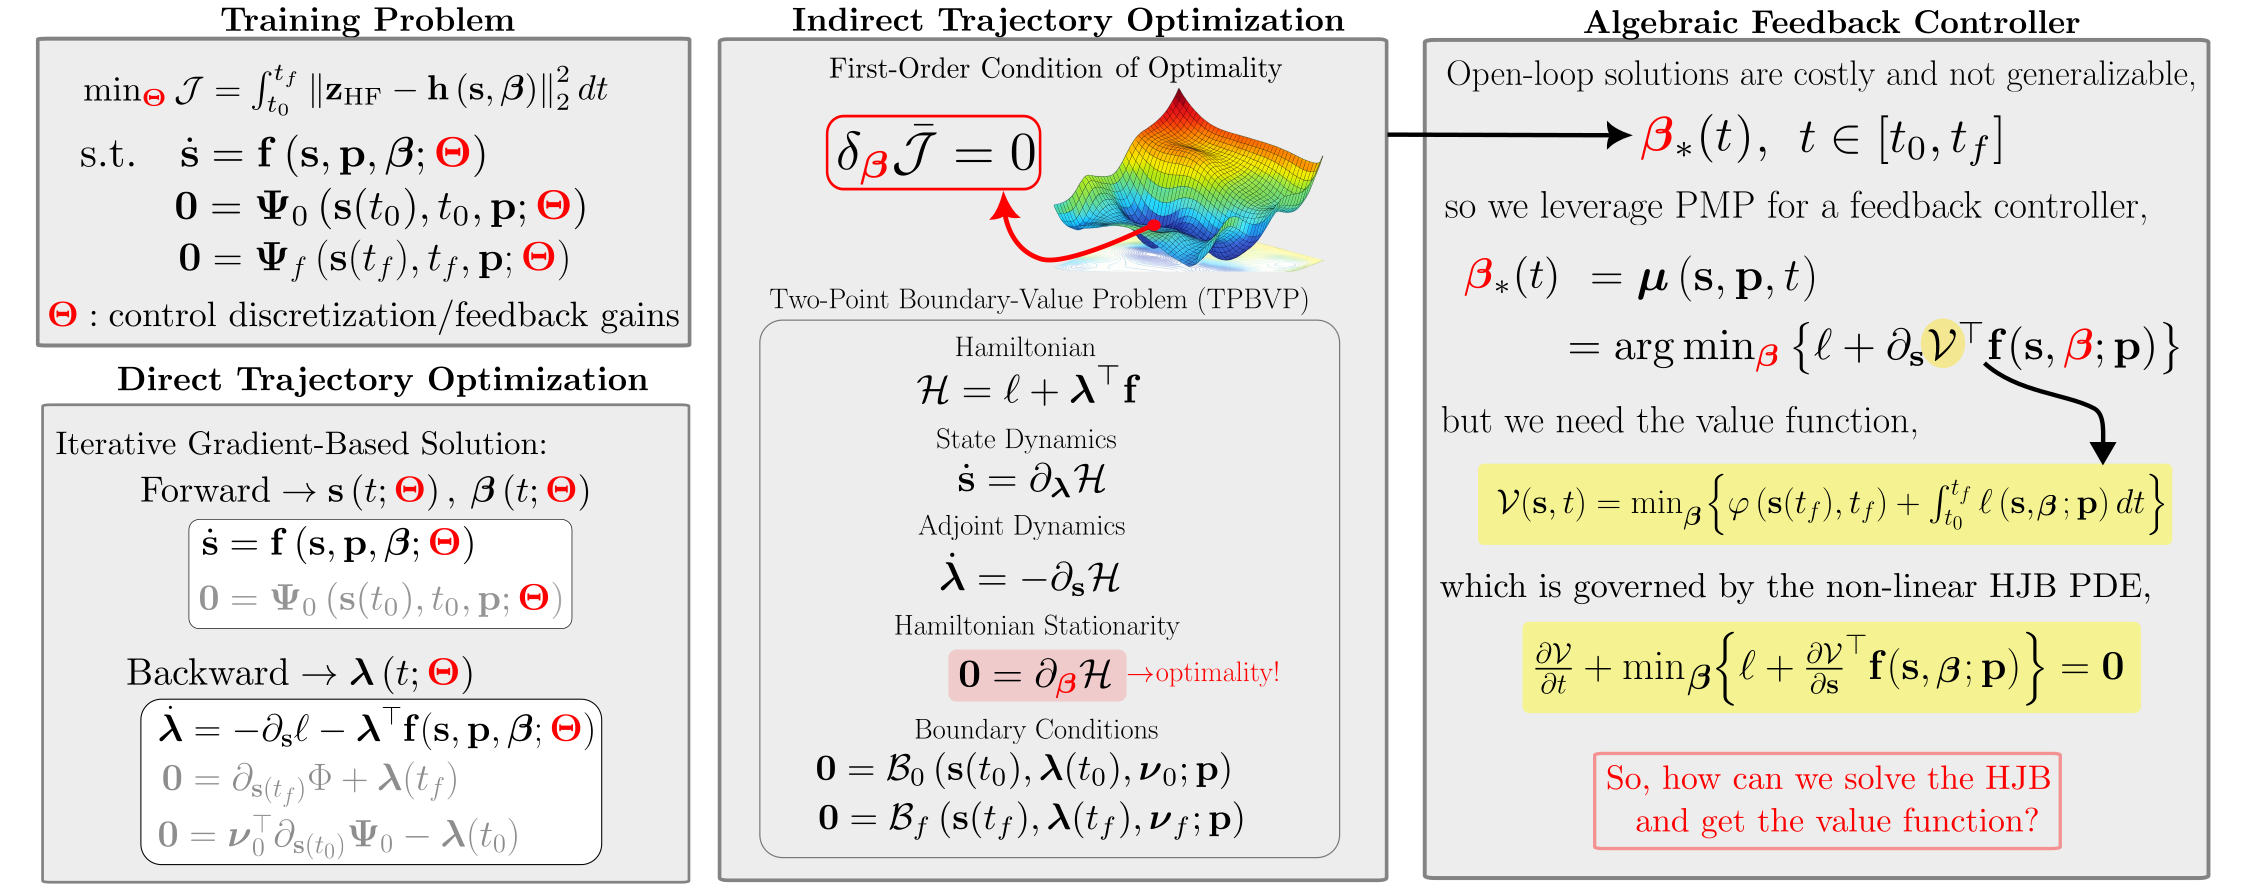
\includegraphics[width=0.95\textwidth]{../figs/ct/ct_overview_19.png}
        \end{figure}}
    \visible<2->{
    \begin{center}
        {\tiny
        $\vs$: state, $\Phi$: penalized terminal constraint, $\vbeta$: control action, $\cB_0,\cB_f$: boundary conditions, $\vnu$: Lagrange multipliers, $\vf$: non-linear dynamics, $\bar{\cJ}$: augmented cost functional, PMP: Pontryagin's Minimum Principle, HJB: Hamilton-Jacobi-Bellman
        }
    \end{center}}
\end{frame}

% \begin{frame}{\small Content Overview}
%     \footnotesize
%     \begin{enumerate}
%         \item \textcolor{gray!50}{Motivation, Background, and Objectives}
%         \item \textcolor{gray!50}{Addressing the Impossible Trinity of Modeling (ITM)}
%         \item \textcolor{gray!50}{Unified Control-Theoretic Training}
%         \item \colorbox{yellow!70}{\textbf{Addressing the Impossible Trinity of Optimal Control (ITOC)}}
%         \item \textcolor{gray!50}{Conclusions and Future Work}
%     \end{enumerate}
% \end{frame}

\begin{frame}
    \centering
    \Large\textbf{Addressing the Impossible Trinity of Optimal Control}
\end{frame}

\begin{frame}{\small How can we leverage the \textbf{control-theoretic} training for optimal closed-loop control?}
    \visible<2->{
    \begin{center}
        {\small \textbf{Consider the following example}:}\\
        {\small On-board optimal closed-loop control of a hypersonic vehicle}
    \end{center}
    \begin{figure}
        \centering
        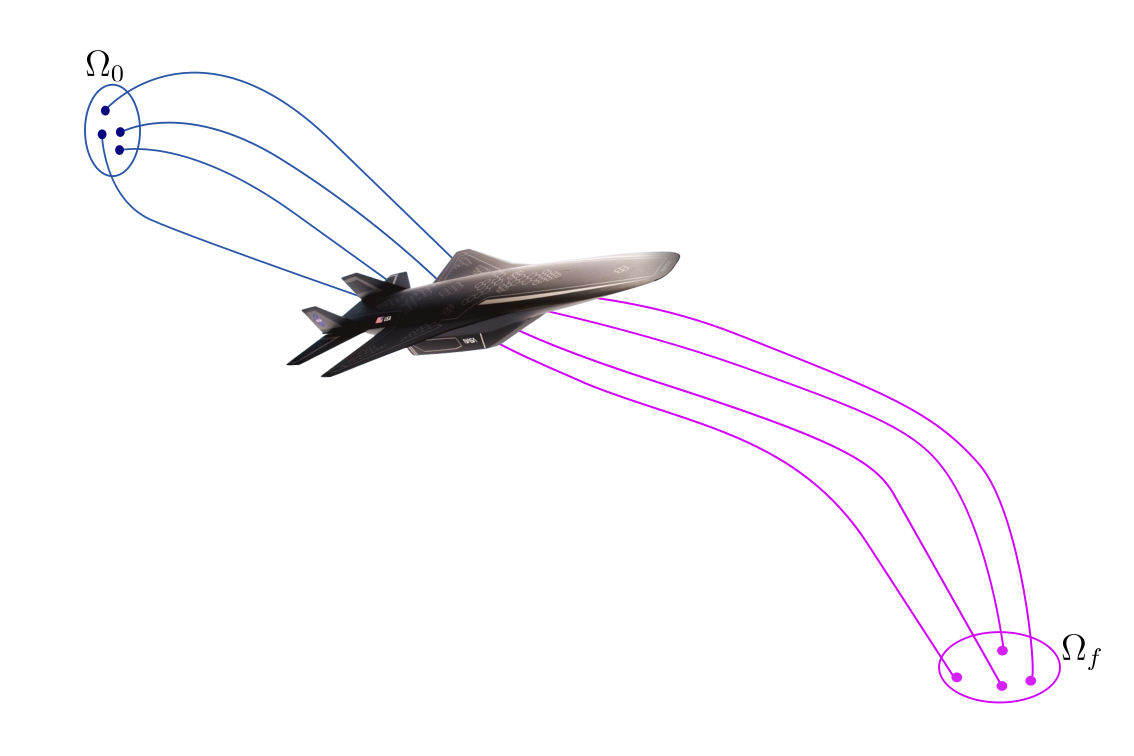
\includegraphics[width=0.6\textwidth]{../figs/introduction/motivating_example_1.png}
    \end{figure}}
\end{frame}

\begin{frame}{\small We want \textbf{accuracy, efficient, and generalizable} solutions to \textbf{non-linear OCPs},}
    \footnotesize
    \begin{columns}
        \begin{column}{0.7\textwidth}
            \only<2>{
                \begin{figure}
                    \centering
                    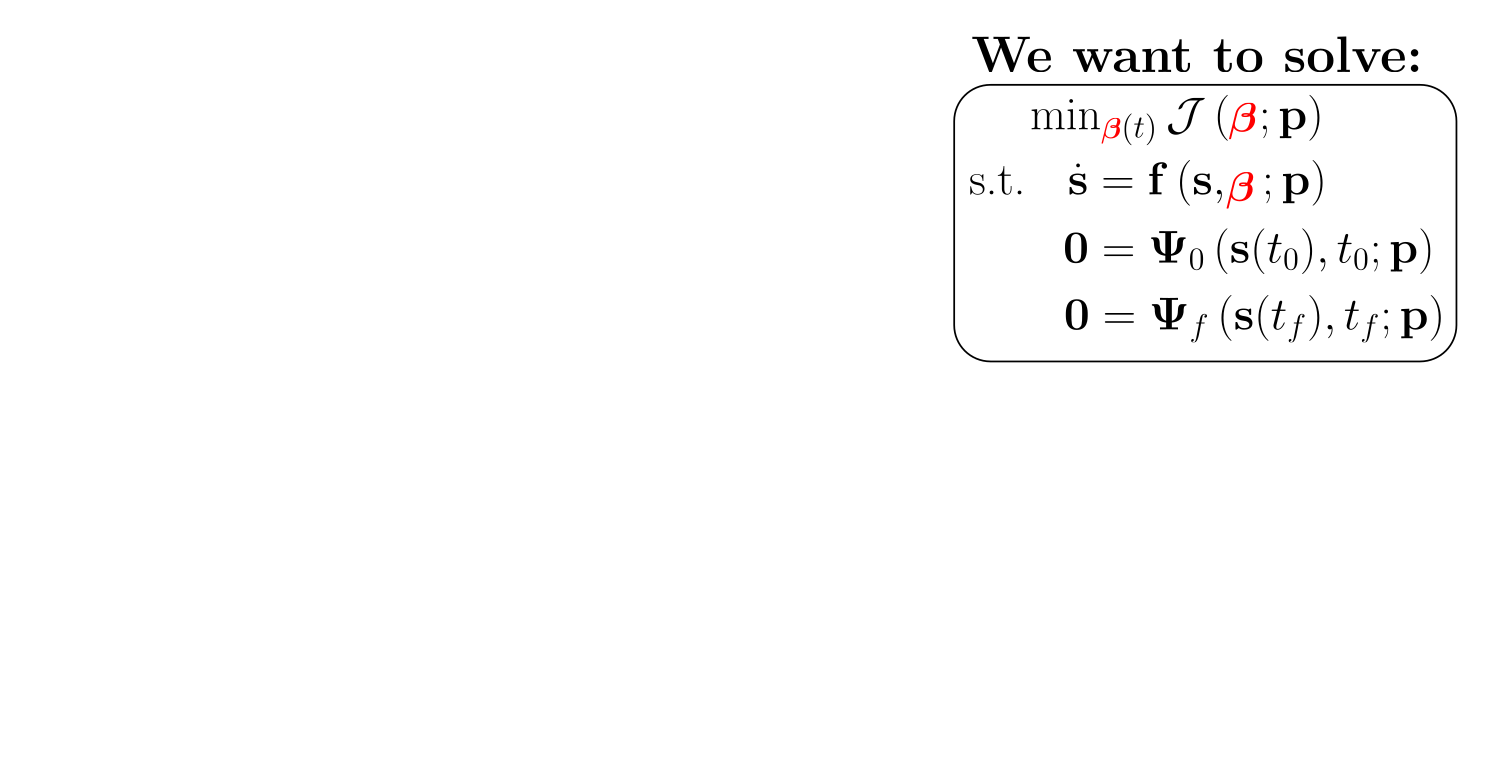
\includegraphics[width=0.9\textwidth]{../figs/sparsehjb/trajectory_parametrization_1.png}
                \end{figure}}
            \only<3>{
                \begin{figure}
                    \centering
                    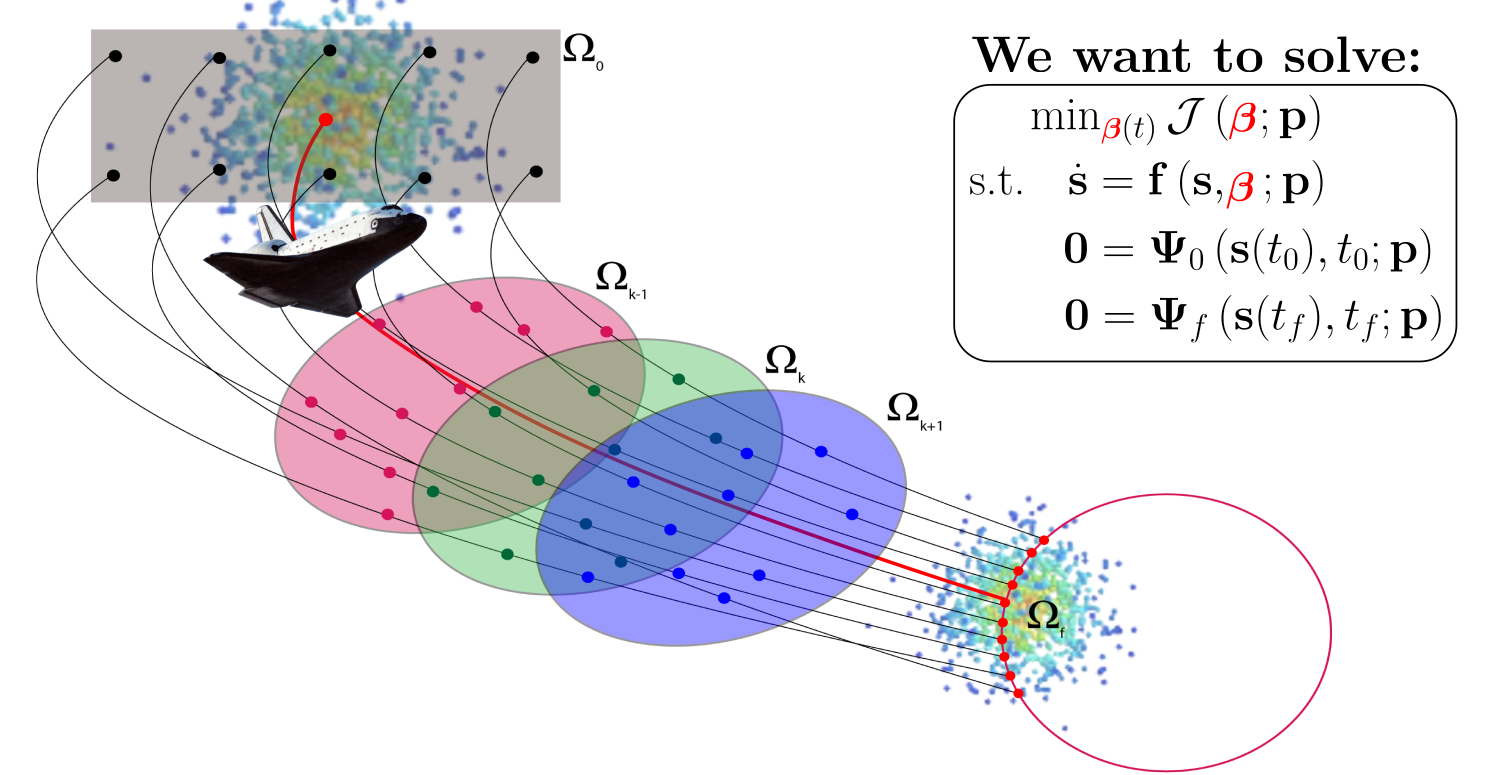
\includegraphics[width=0.9\textwidth]{../figs/sparsehjb/trajectory_parametrization_2.png}
                \end{figure}}
            \only<4->{
                \begin{figure}
                    \centering
                    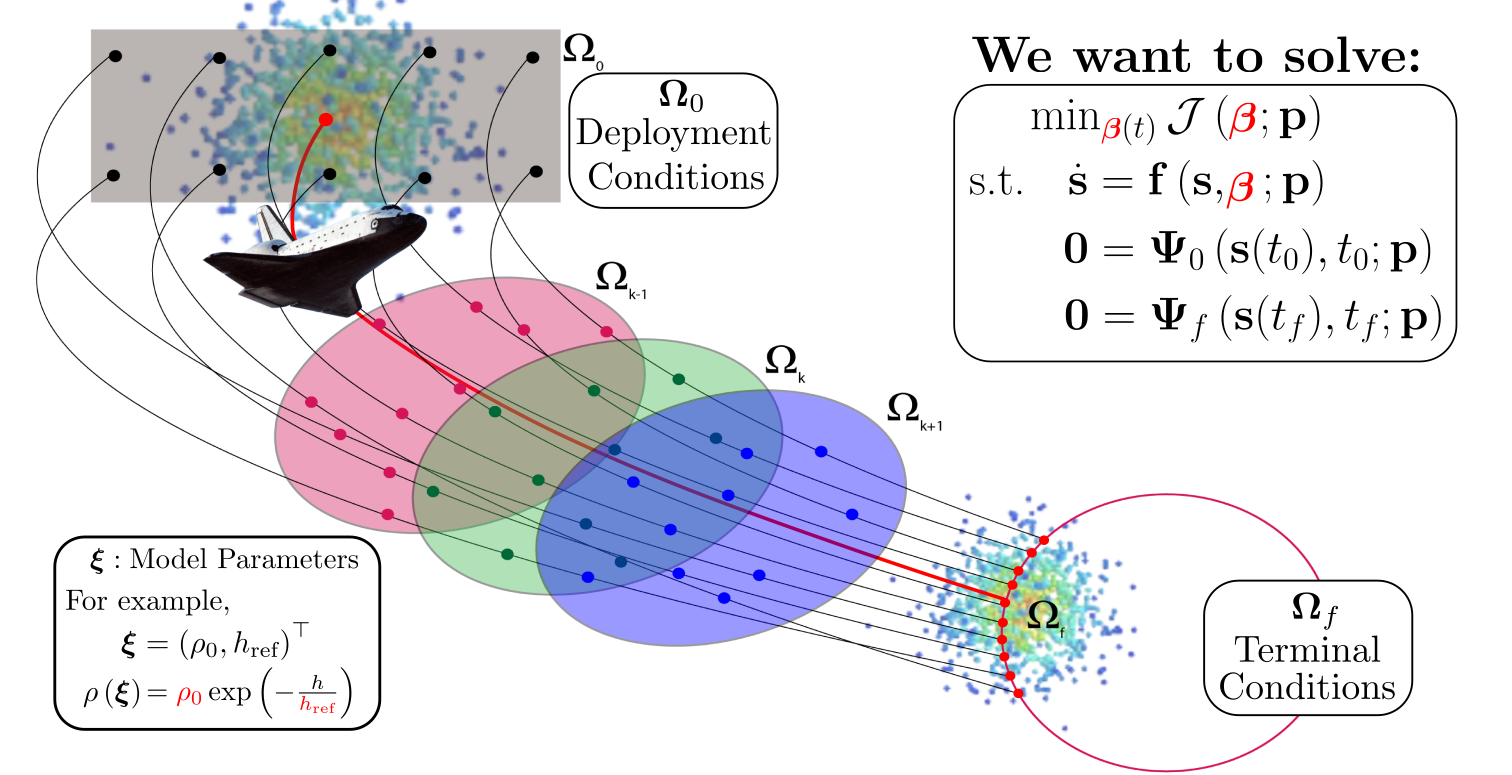
\includegraphics[width=0.9\textwidth]{../figs/sparsehjb/trajectory_parametrization_3.png}
                \end{figure}}
        \end{column}
        \hspace*{-0.5in}
        \begin{column}{0.4\textwidth}
            \visible<5->{
            \begin{graybox}{Parametrization}
                \visible<6->{
                Parameters,
                \begin{equation*}
                    \vp = \left(\vOmega_0,\vOmega_f,\vxi\right)^\top\in\mathbb{R}^{n_p}
                \end{equation*}}
                \visible<7->{
                are, e.g., normally distributed,
                \begin{equation*}
                    \vp\sim\mathcal{N}\left(\mathbf{m},\boldsymbol{\sigma}\right)
                \end{equation*}}
                \visible<8->{
                where,
                \begin{itemize}
                    \item $\mathbf{m}$: nominal mission,
                    \item $\boldsymbol{\sigma}$: mission uncertainty
                \end{itemize}}
            \end{graybox}}
        \end{column}
    \end{columns}
\end{frame}

\begin{frame}{\small Generate a sparse high fidelity \textbf{distribution of optimal paths},}
    \footnotesize
    \only<1>{
        \begin{figure}
            \centering
            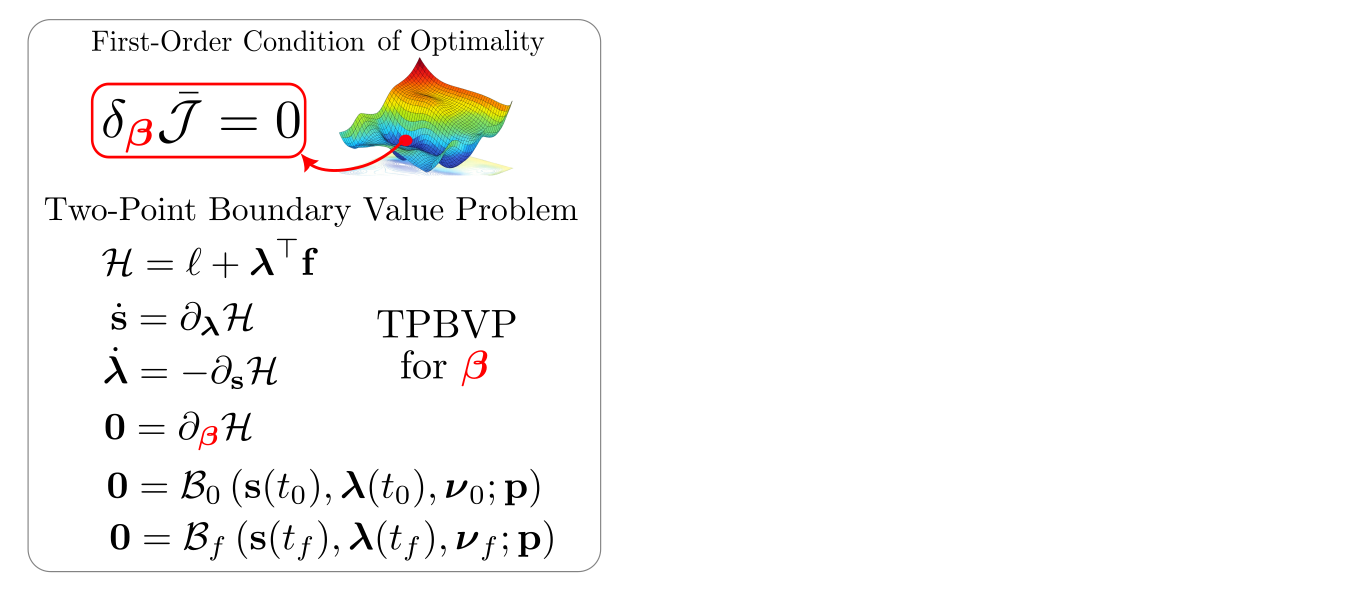
\includegraphics[width=0.9\textwidth]{../figs/sparsehjb/solutions_1.png}
        \end{figure}}
    \only<2>{
        \begin{figure}
            \centering
            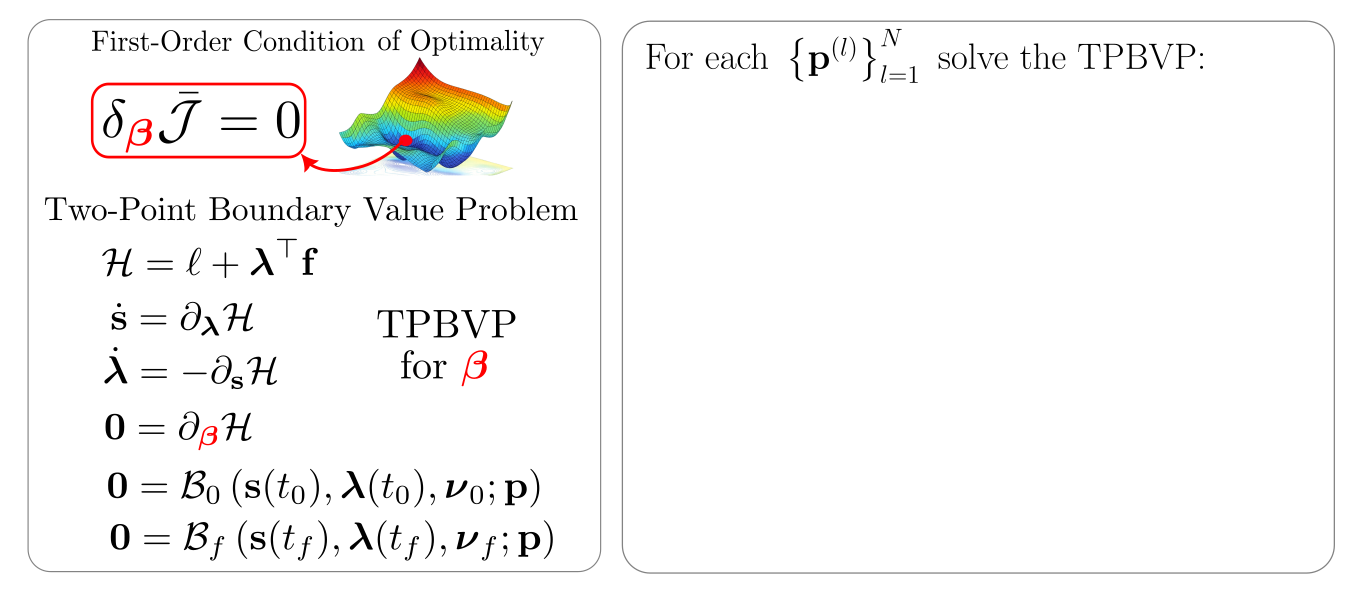
\includegraphics[width=0.9\textwidth]{../figs/sparsehjb/solutions_2.png}
        \end{figure}}
    \only<3>{
        \begin{figure}
            \centering
            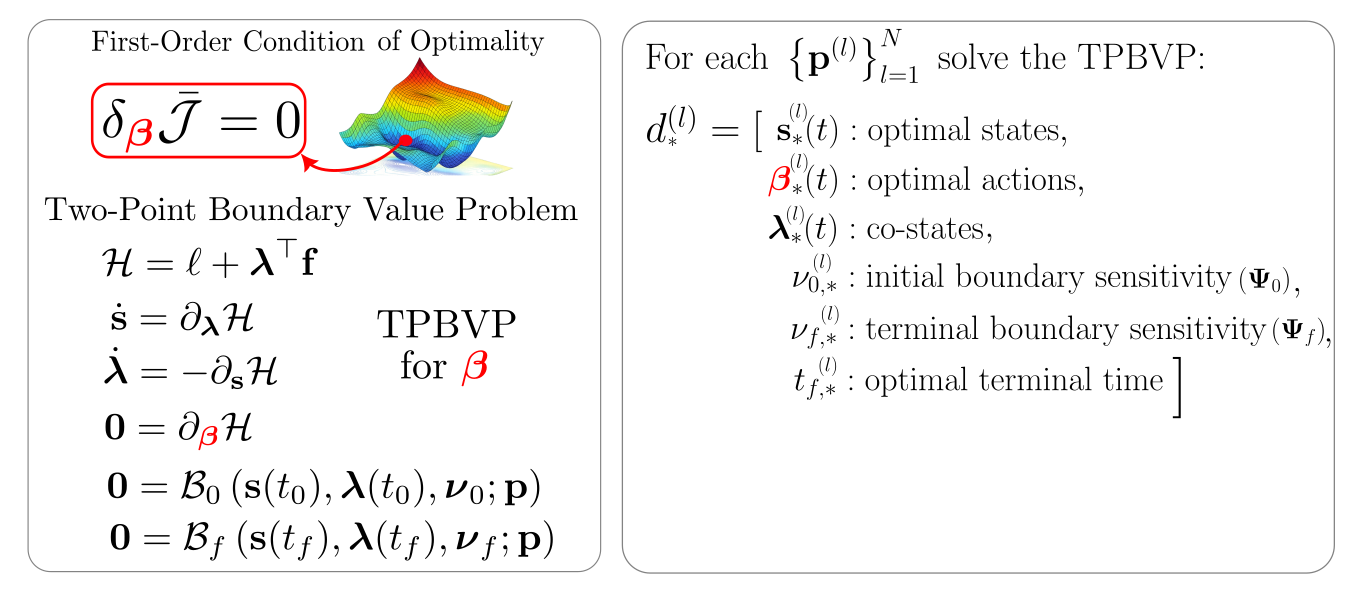
\includegraphics[width=0.9\textwidth]{../figs/sparsehjb/solutions_3.png}
        \end{figure}}
    \only<4>{
        \begin{figure}
            \centering
            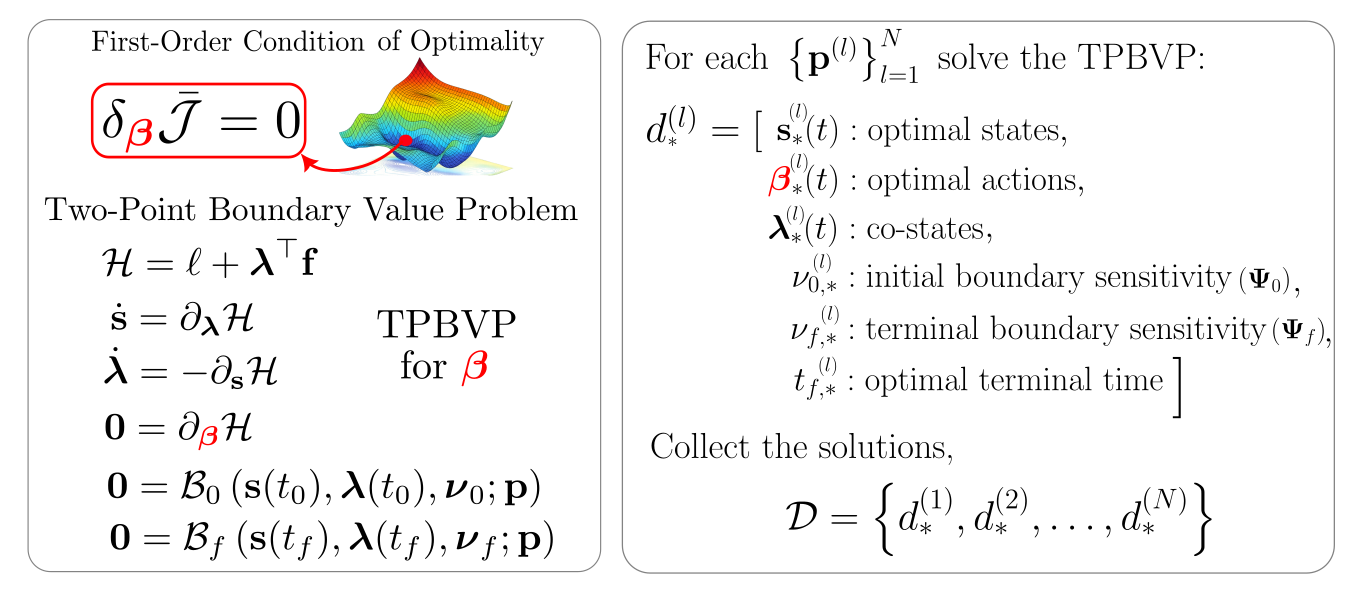
\includegraphics[width=0.9\textwidth]{../figs/sparsehjb/solutions_4.png}
        \end{figure}}
\end{frame}

\begin{frame}{\small \textbf{Learn the value function} from the sparse high fidelity data,}
    \footnotesize
    \only<2>{
        \begin{figure}
            \centering
            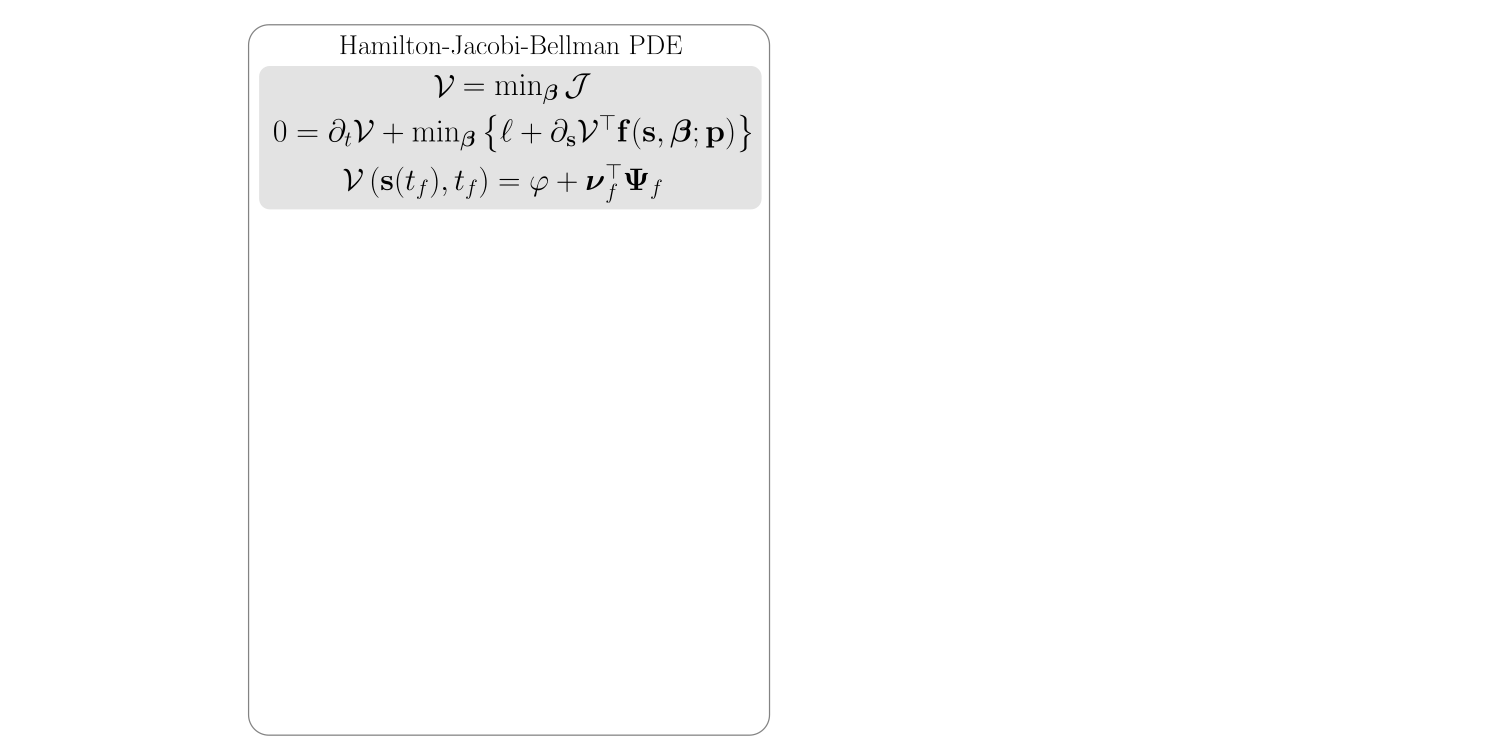
\includegraphics[width=0.95\textwidth]{../figs/sparsehjb/characteristics_1.png}
        \end{figure}}
    \only<3>{
        \begin{figure}
            \centering
            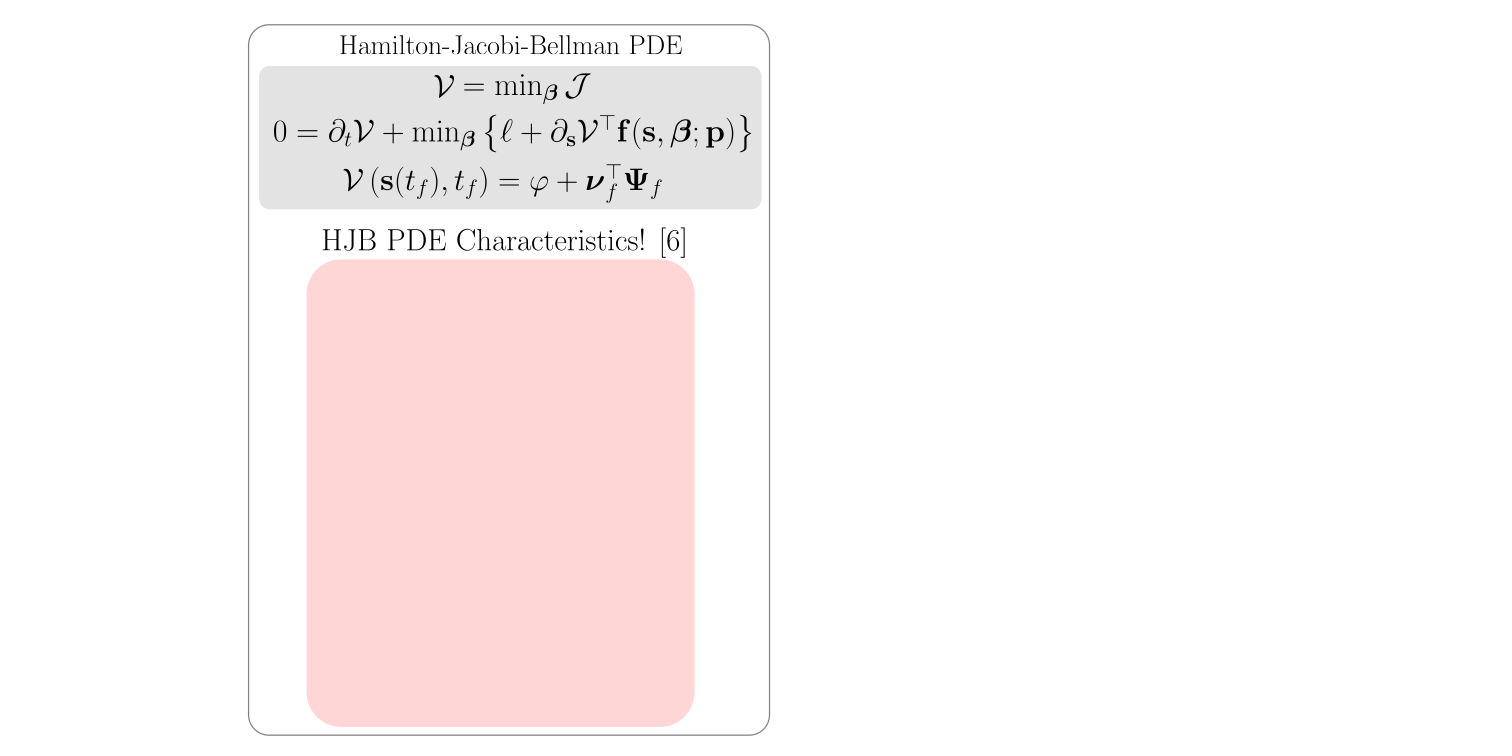
\includegraphics[width=0.95\textwidth]{../figs/sparsehjb/characteristics_2.png}
        \end{figure}}
    \only<4>{
        \begin{figure}
            \centering
            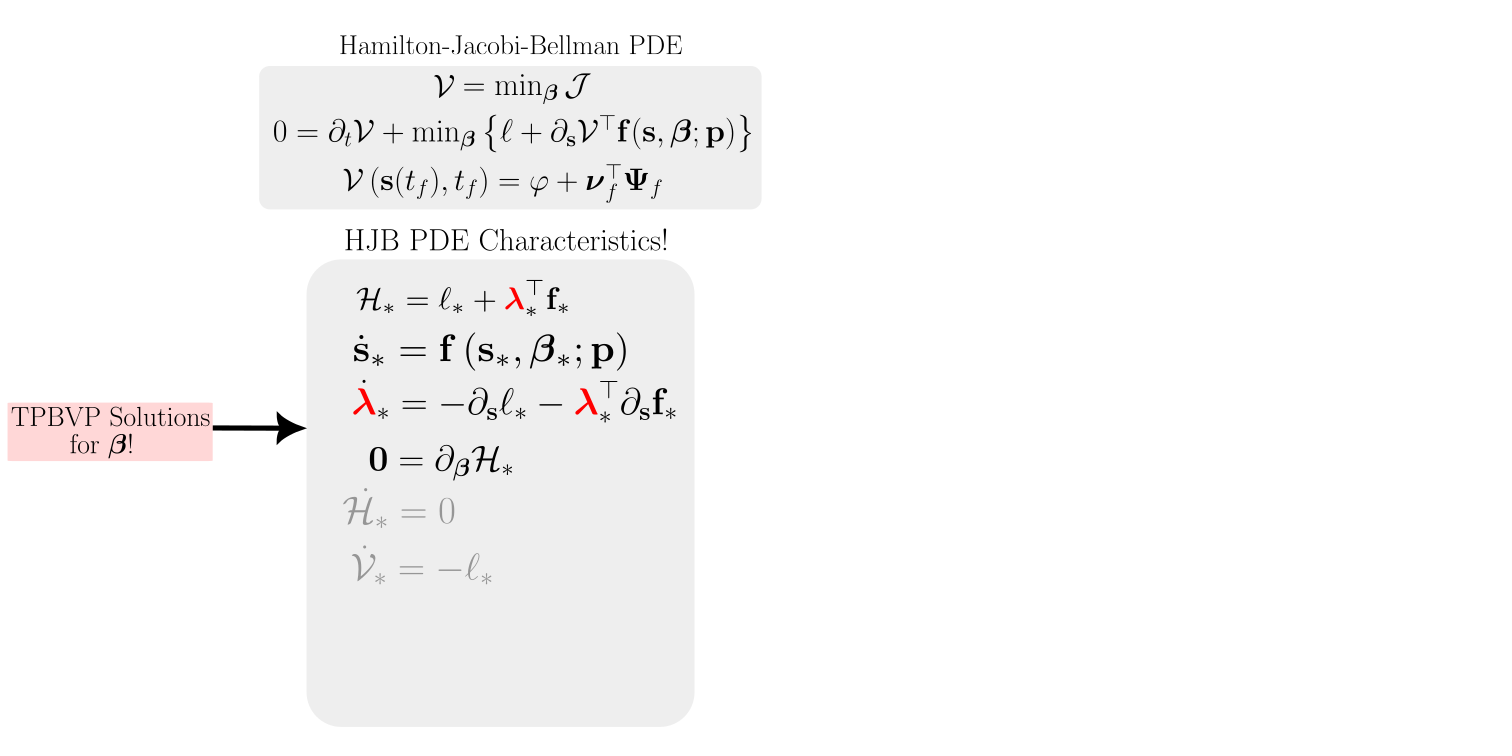
\includegraphics[width=0.95\textwidth]{../figs/sparsehjb/characteristics_3.png}
        \end{figure}}
    \only<5>{
        \begin{figure}
            \centering
            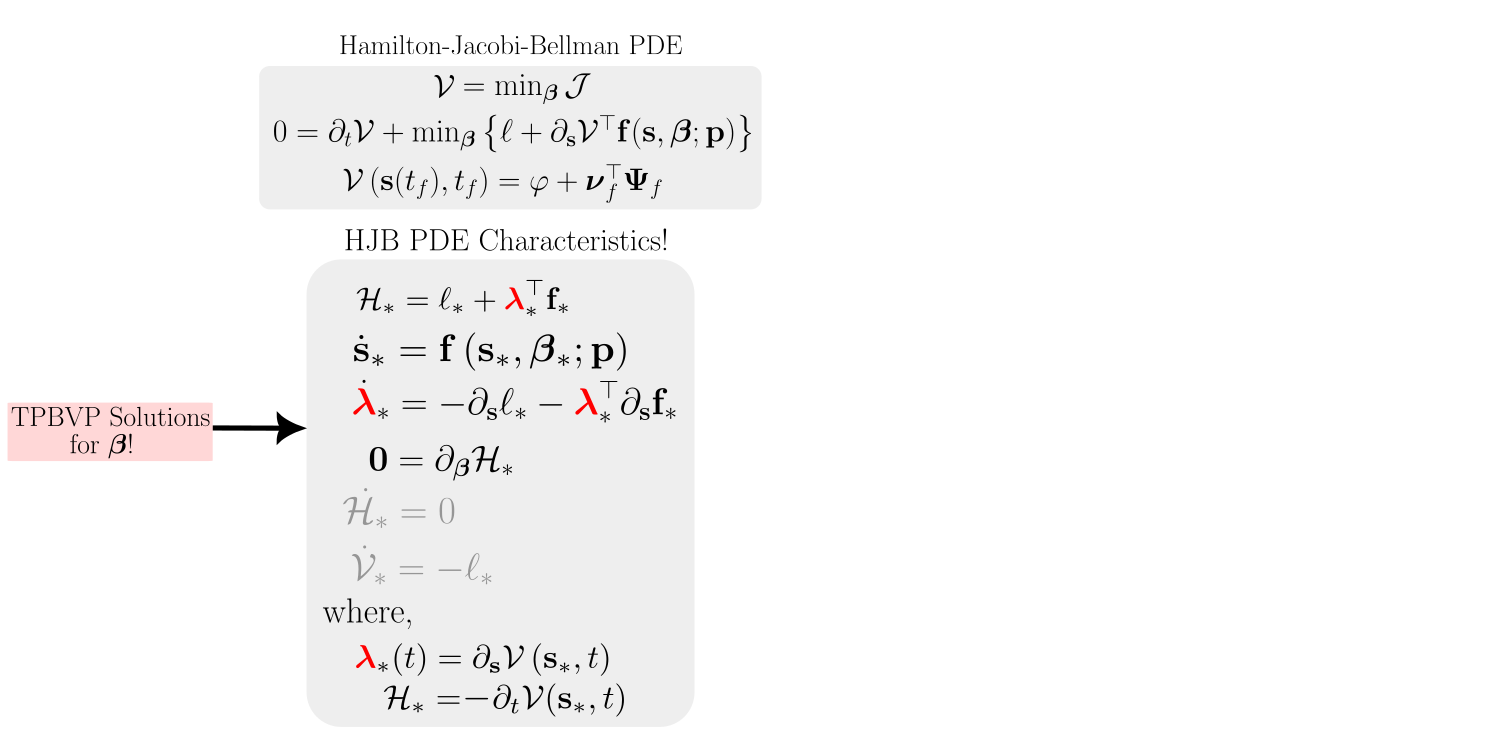
\includegraphics[width=0.95\textwidth]{../figs/sparsehjb/characteristics_4.png}
        \end{figure}}
    \only<6>{
        \begin{figure}
            \centering
            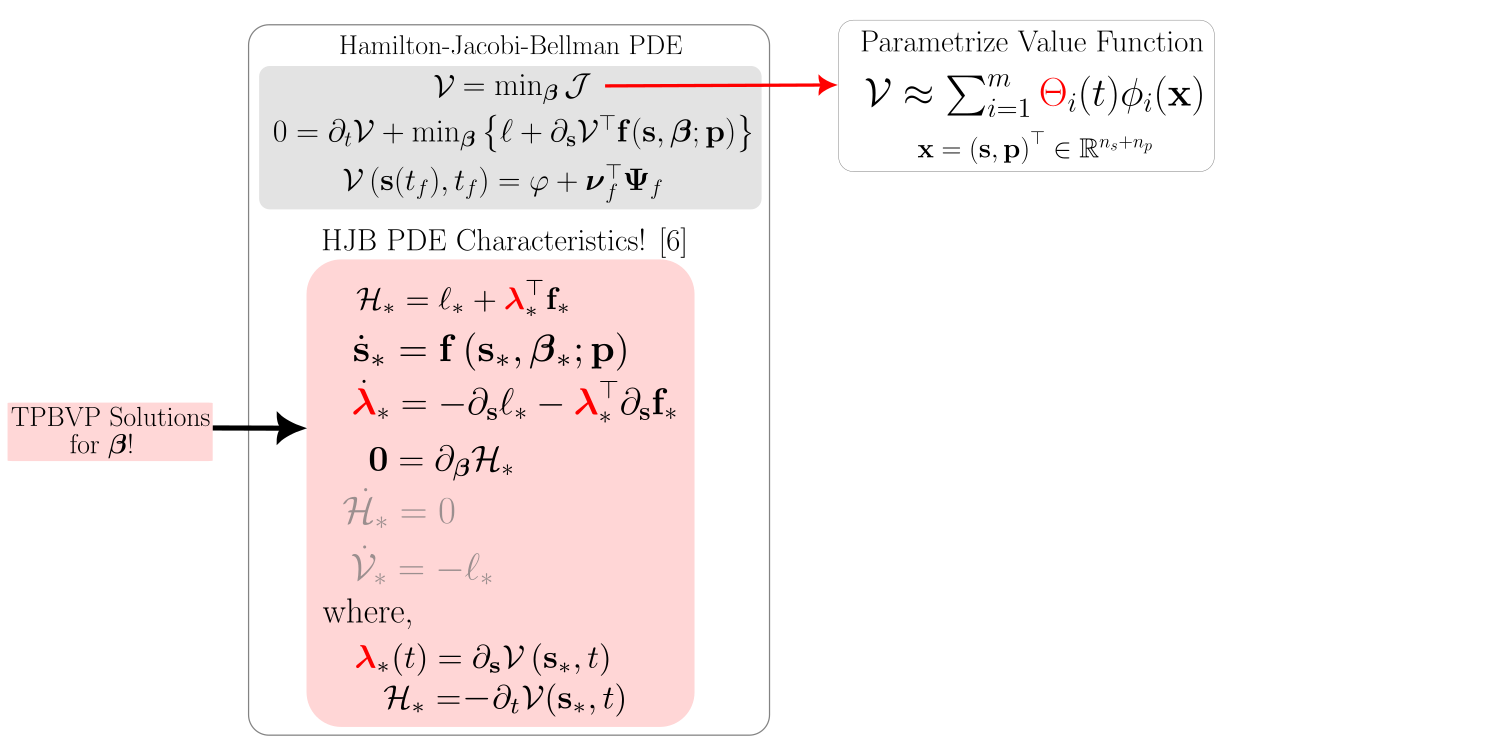
\includegraphics[width=0.95\textwidth]{../figs/sparsehjb/characteristics_5.png}
        \end{figure}}
    \only<7>{
        \begin{figure}
            \centering
            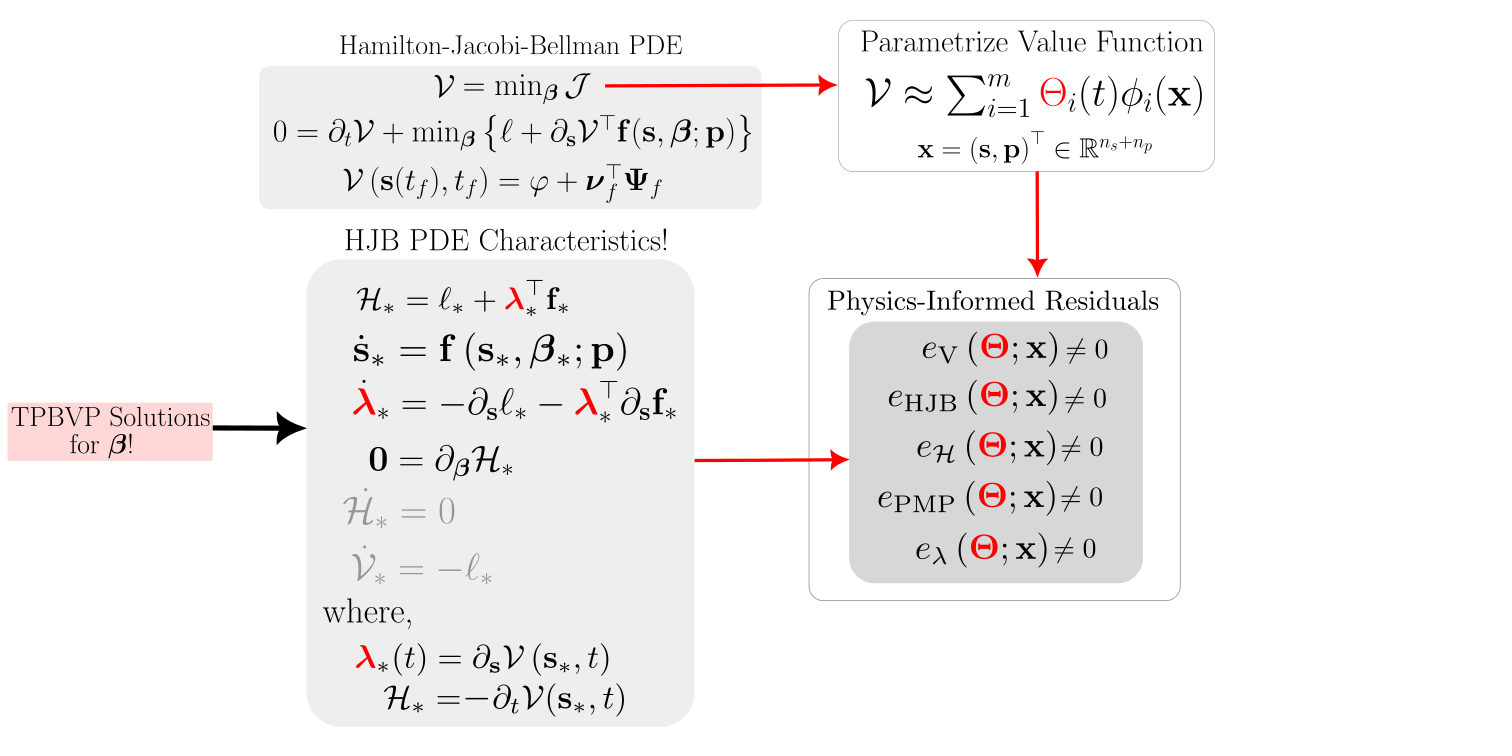
\includegraphics[width=0.95\textwidth]{../figs/sparsehjb/characteristics_6.png}
        \end{figure}}
    \only<8>{
        \begin{figure}
            \centering
            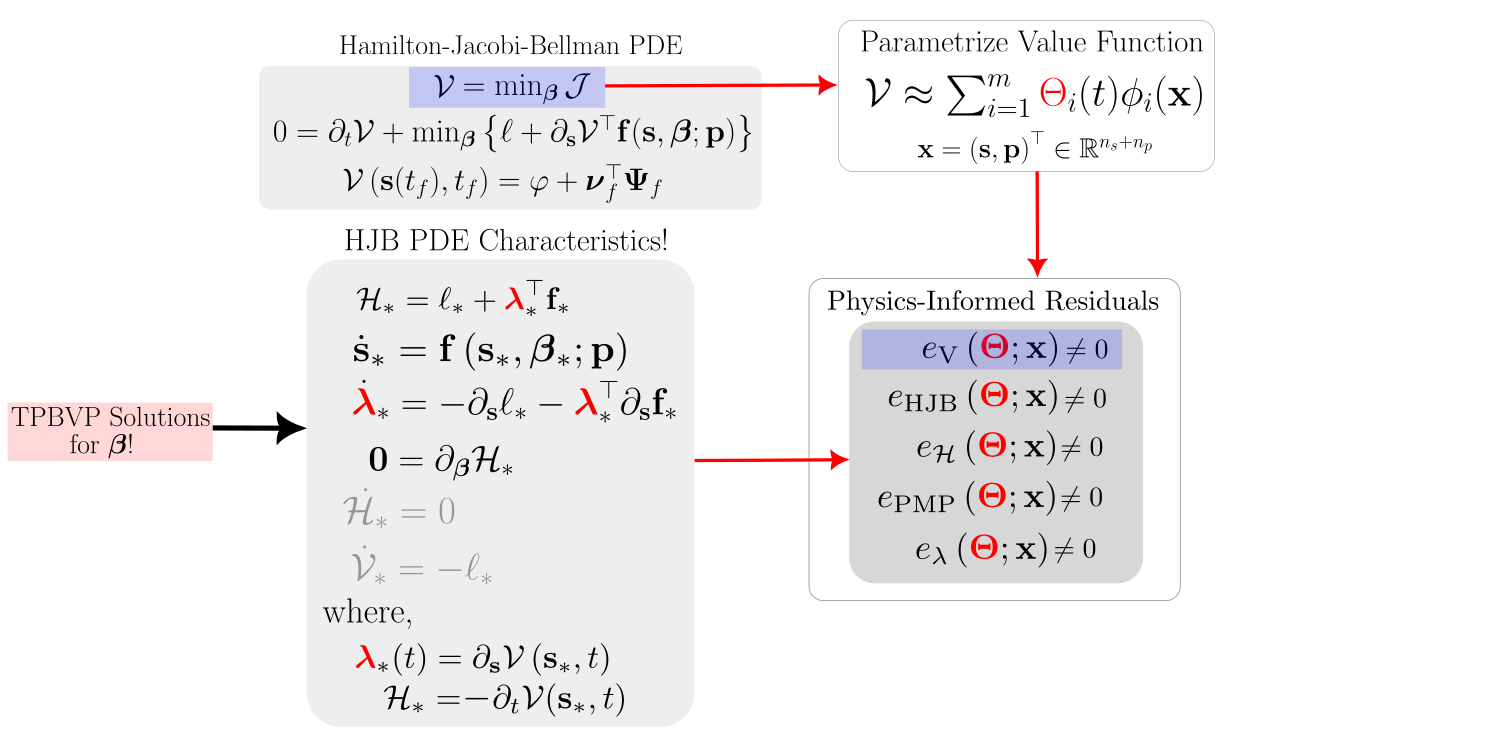
\includegraphics[width=0.95\textwidth]{../figs/sparsehjb/characteristics_7.png}
        \end{figure}}
    \only<9>{
        \begin{figure}
            \centering
            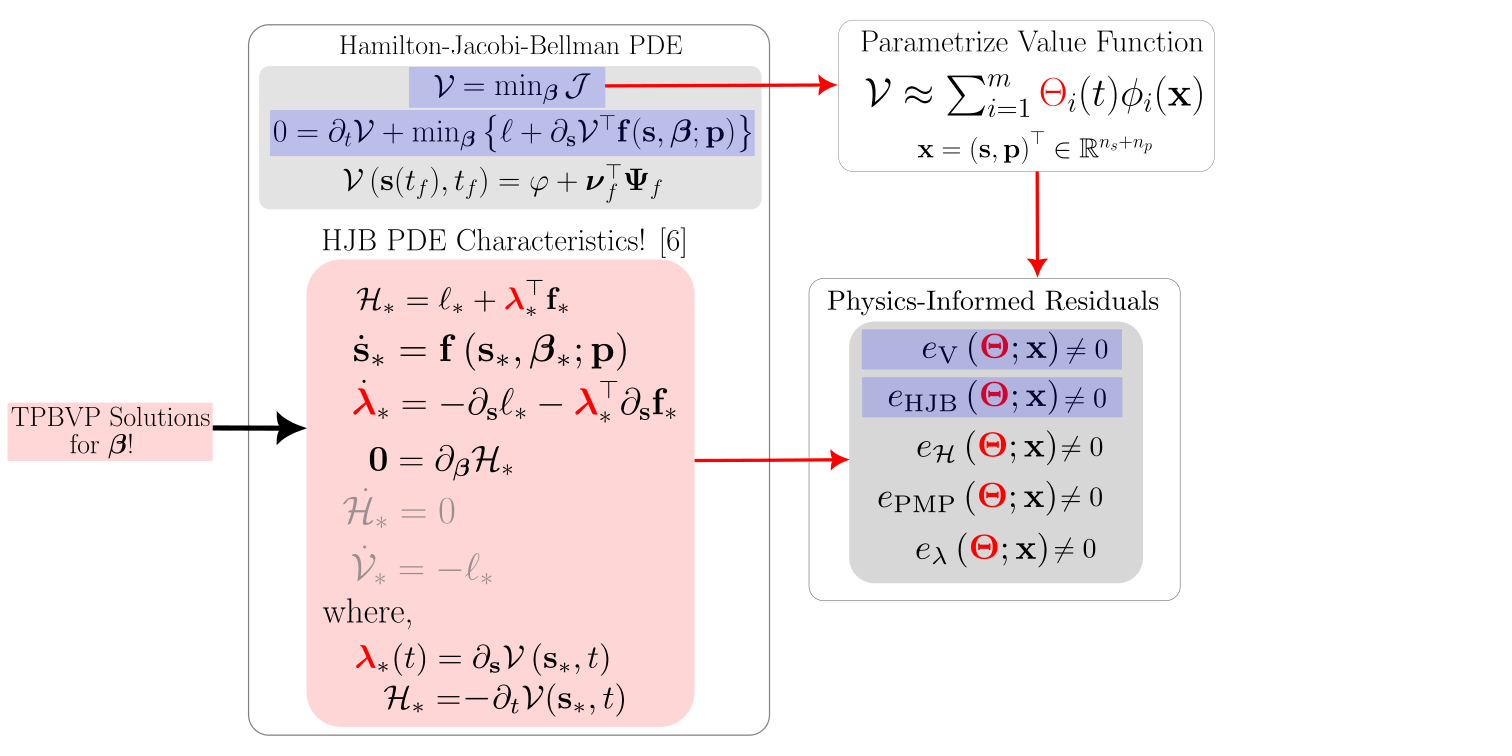
\includegraphics[width=0.95\textwidth]{../figs/sparsehjb/characteristics_8.png}
        \end{figure}}
    \only<10>{
        \begin{figure}
            \centering
            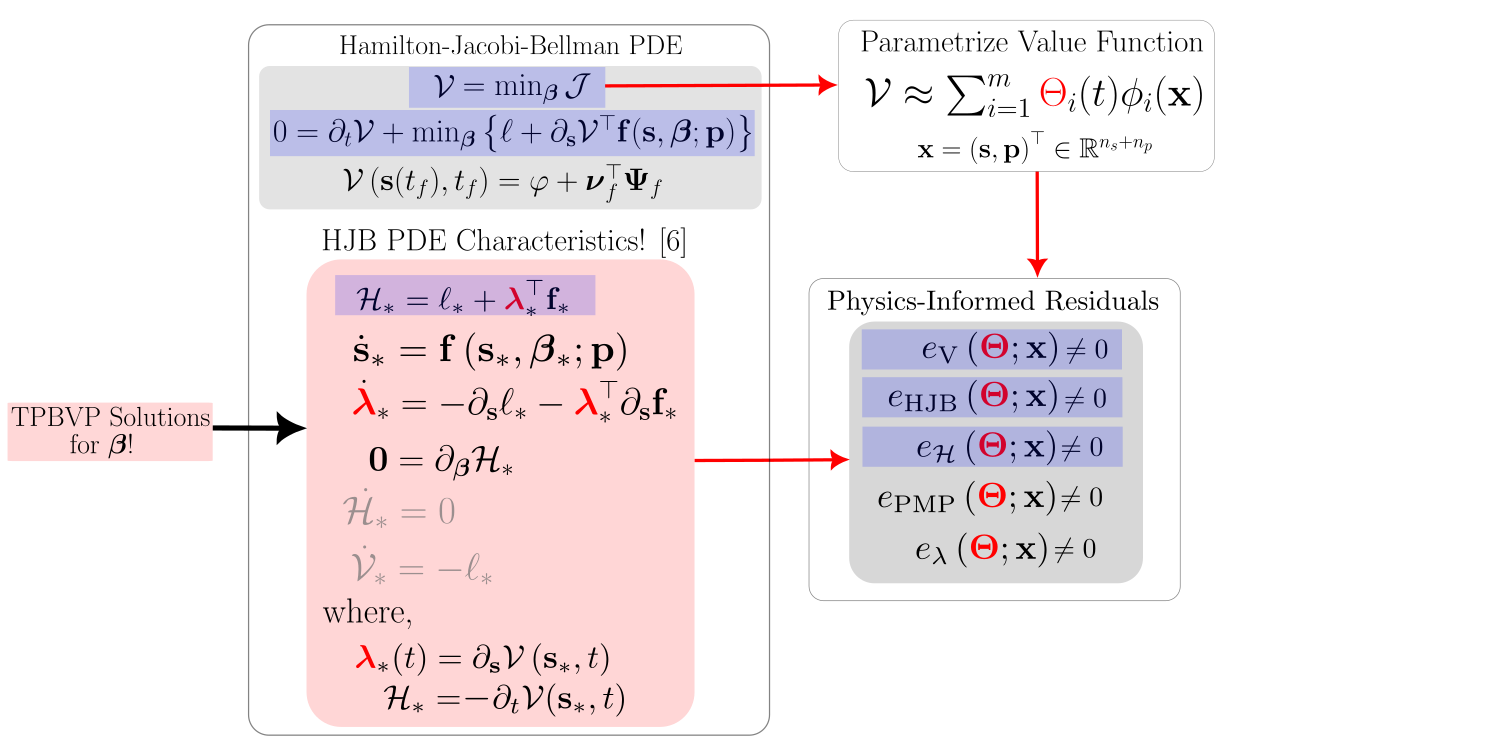
\includegraphics[width=0.95\textwidth]{../figs/sparsehjb/characteristics_9.png}
        \end{figure}}
    \only<11>{
        \begin{figure}
            \centering
            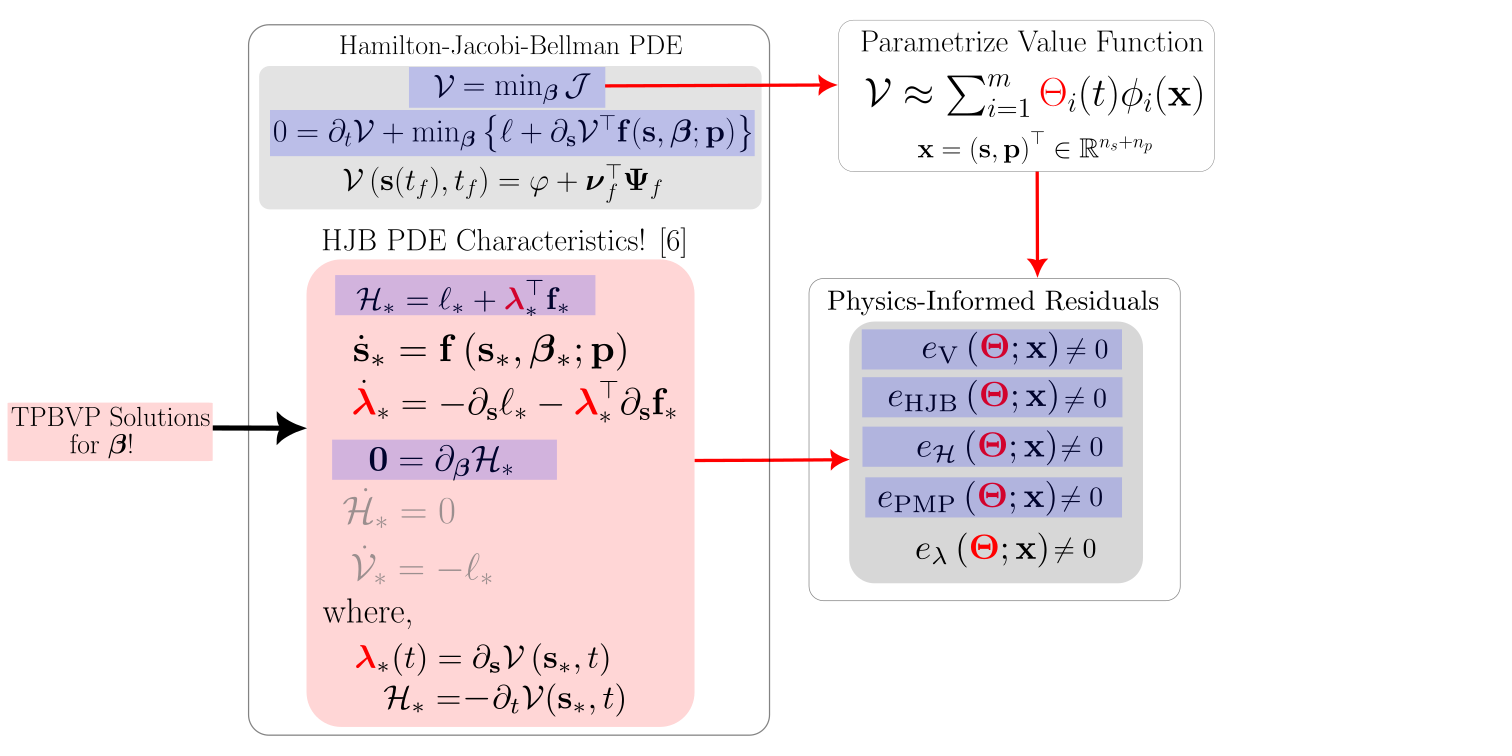
\includegraphics[width=0.95\textwidth]{../figs/sparsehjb/characteristics_10.png}
        \end{figure}}
    \only<12>{
        \begin{figure}
            \centering
            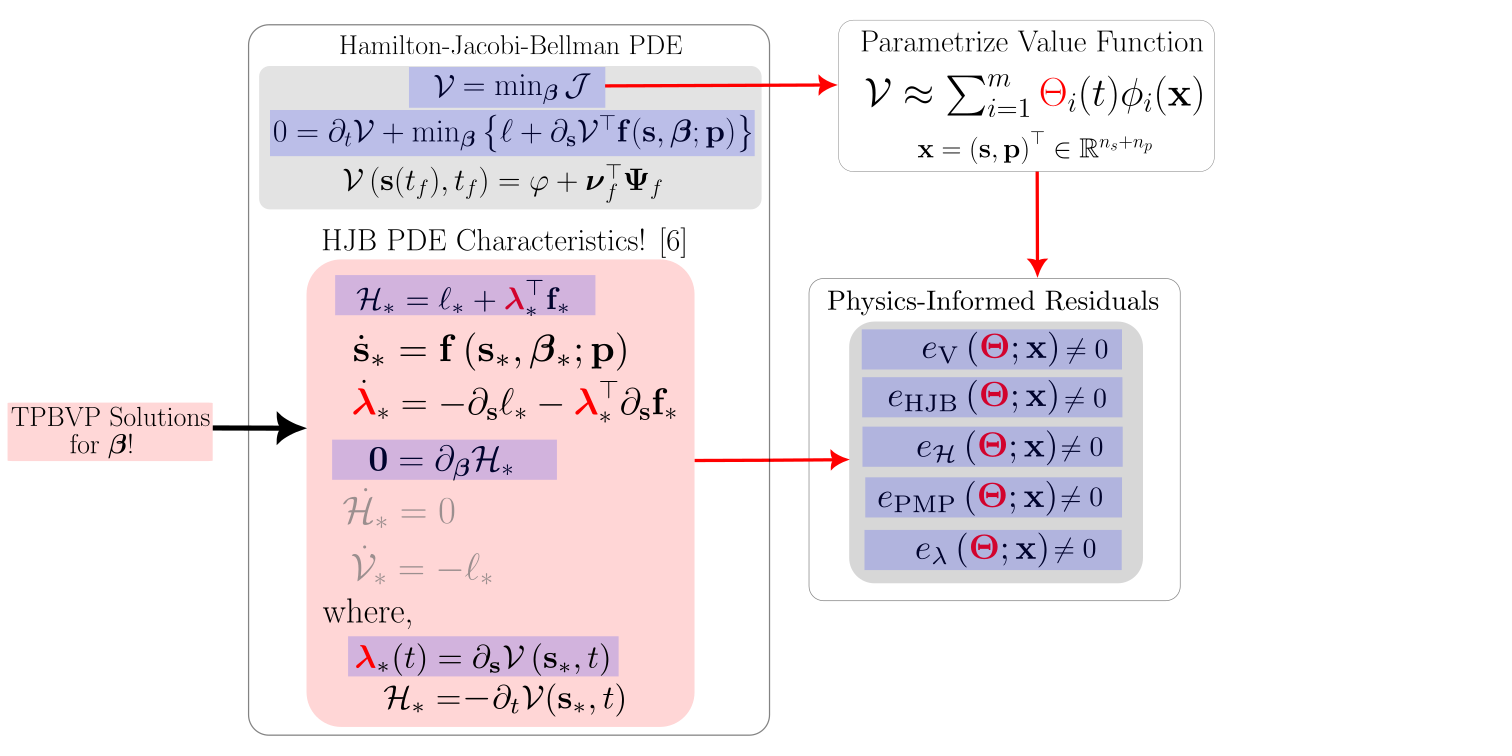
\includegraphics[width=0.95\textwidth]{../figs/sparsehjb/characteristics_11.png}
        \end{figure}}
    \only<13>{
        \begin{figure}
            \centering
            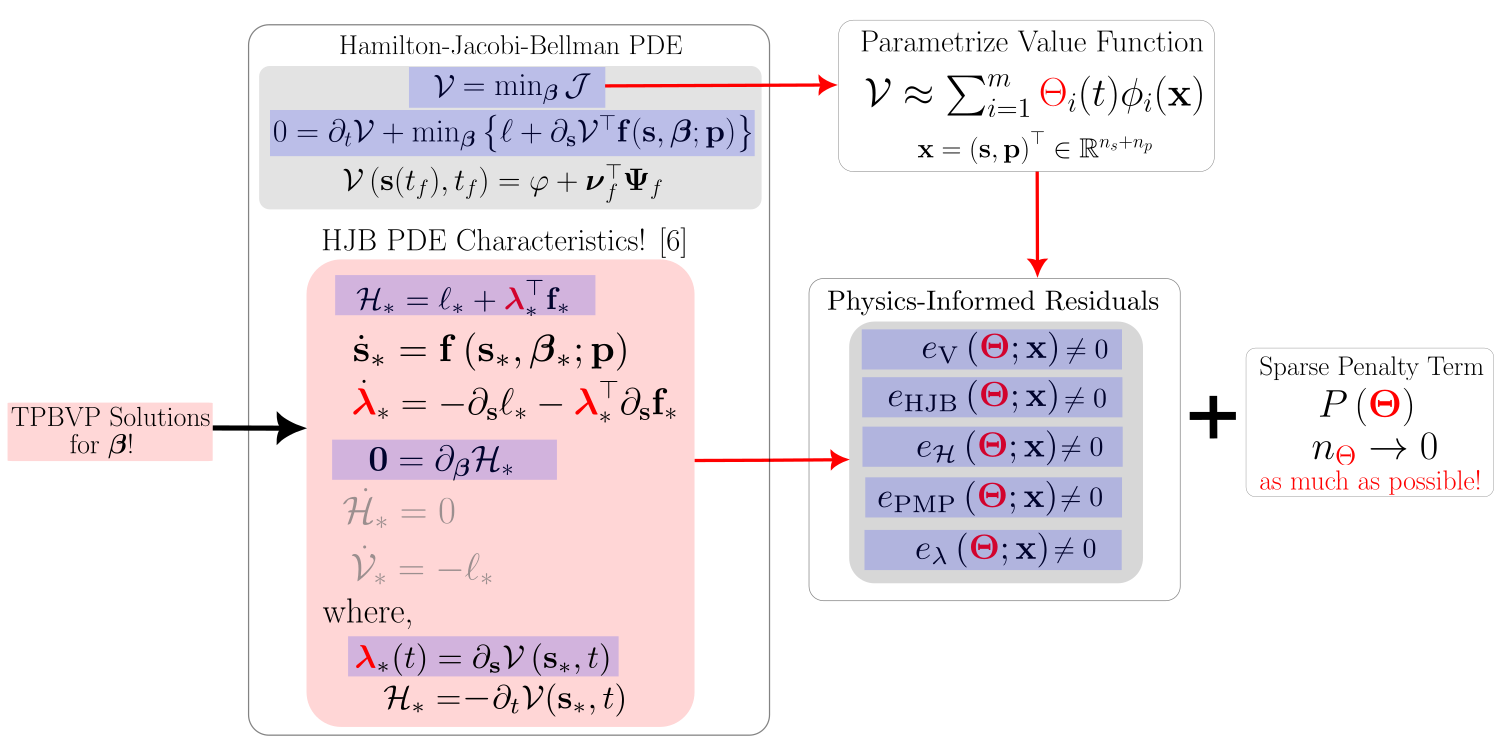
\includegraphics[width=0.95\textwidth]{../figs/sparsehjb/characteristics_12.png}
        \end{figure}}
\end{frame}

\begin{frame}{\small We can \textbf{learn the value function} with controllable \textbf{efficiency and accuracy},}
    \footnotesize
    \only<2>{
        \begin{figure}
            \centering
            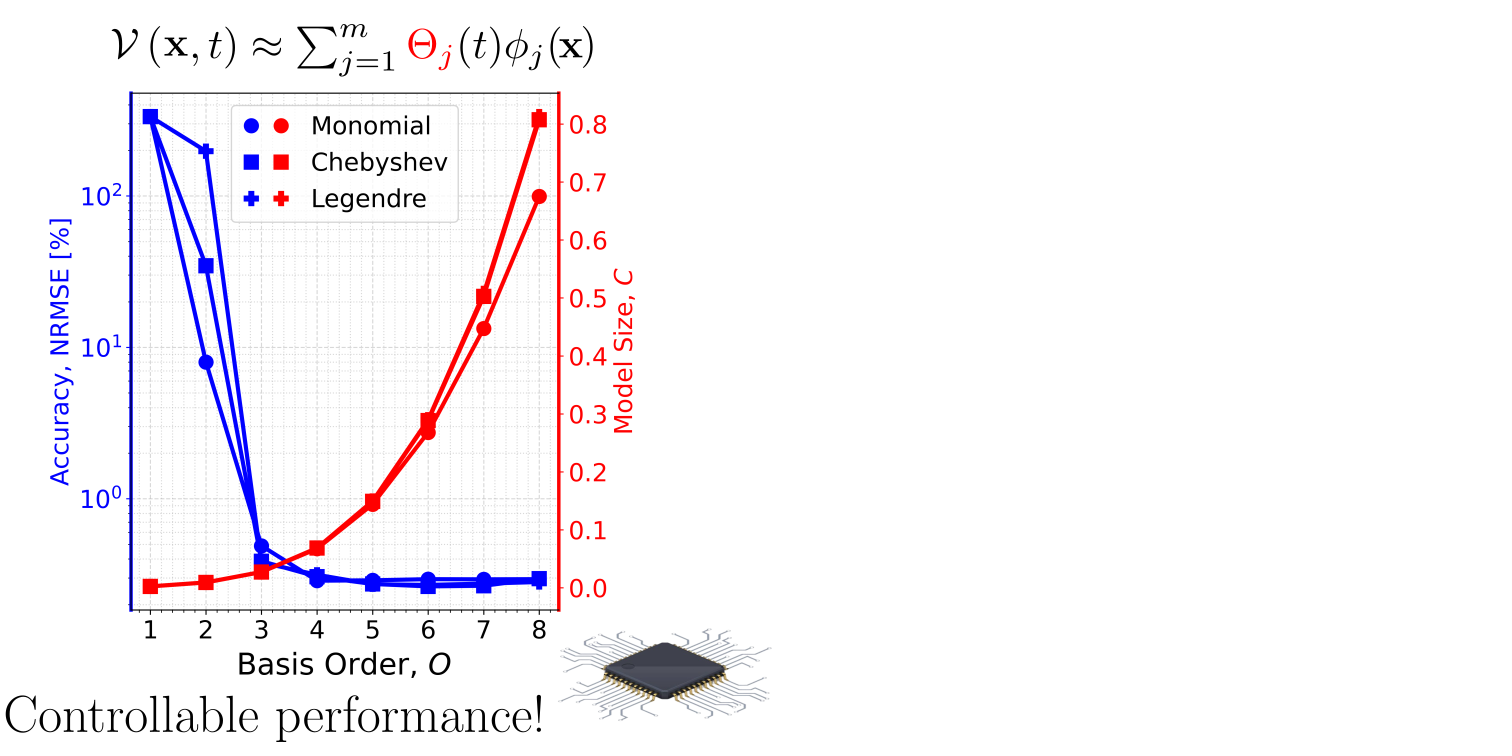
\includegraphics[width=0.9\textwidth]{../figs/sparsehjb/performance_ae_1.png}
        \end{figure}}
    \only<3>{
        \begin{figure}
            \centering
            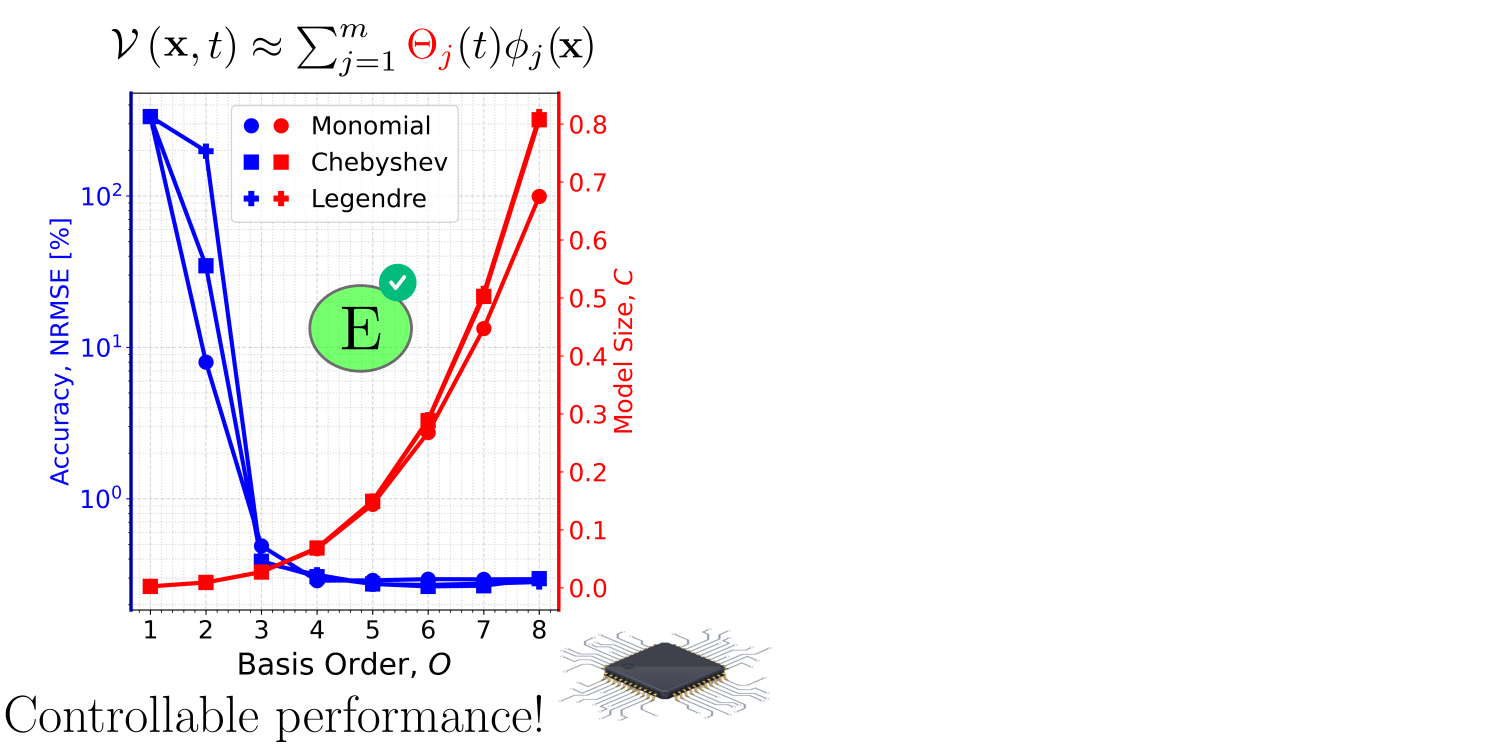
\includegraphics[width=0.9\textwidth]{../figs/sparsehjb/performance_ae_2.png}
        \end{figure}}
    \only<4>{
        \begin{figure}
            \centering
            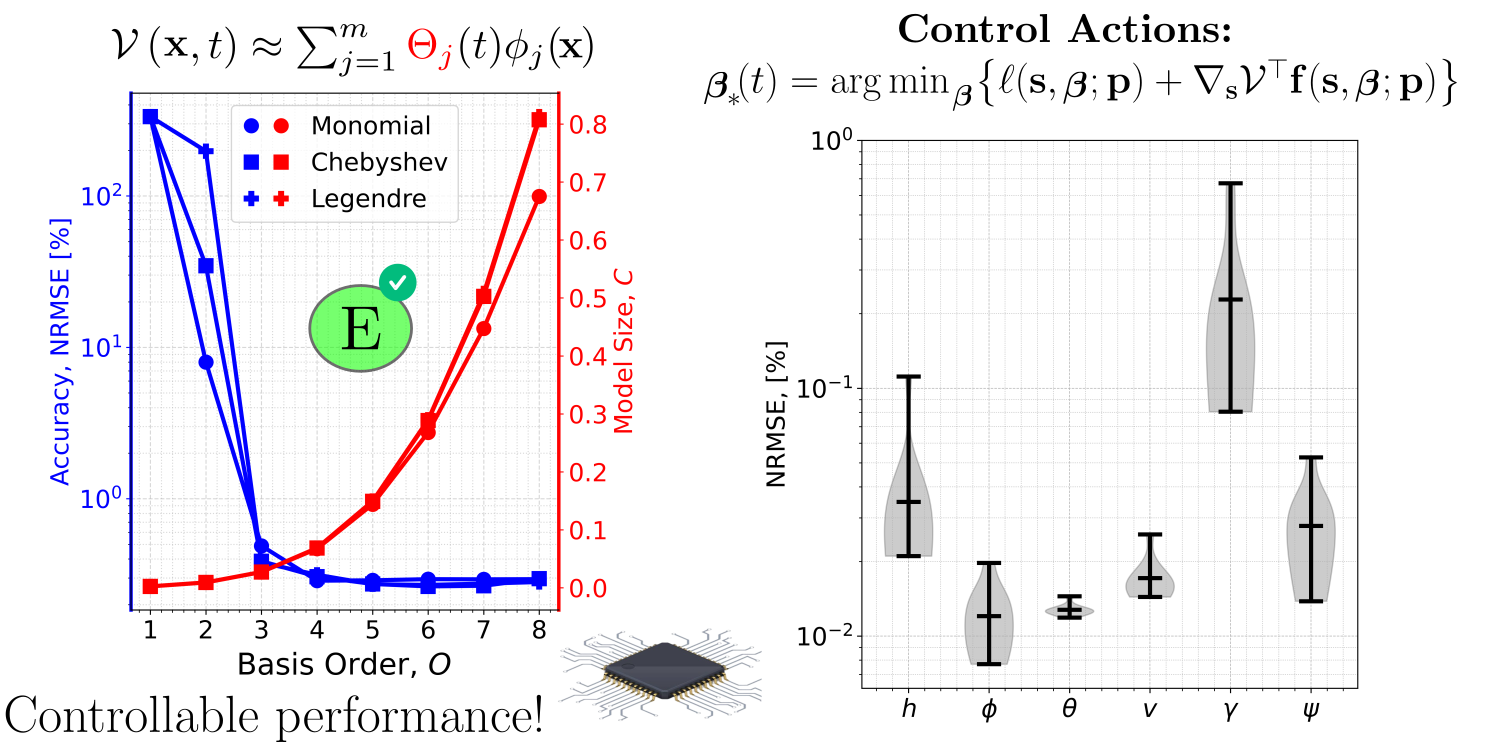
\includegraphics[width=0.9\textwidth]{../figs/sparsehjb/performance_ae_3.png}
        \end{figure}}
    \only<5>{
        \begin{figure}
            \centering
            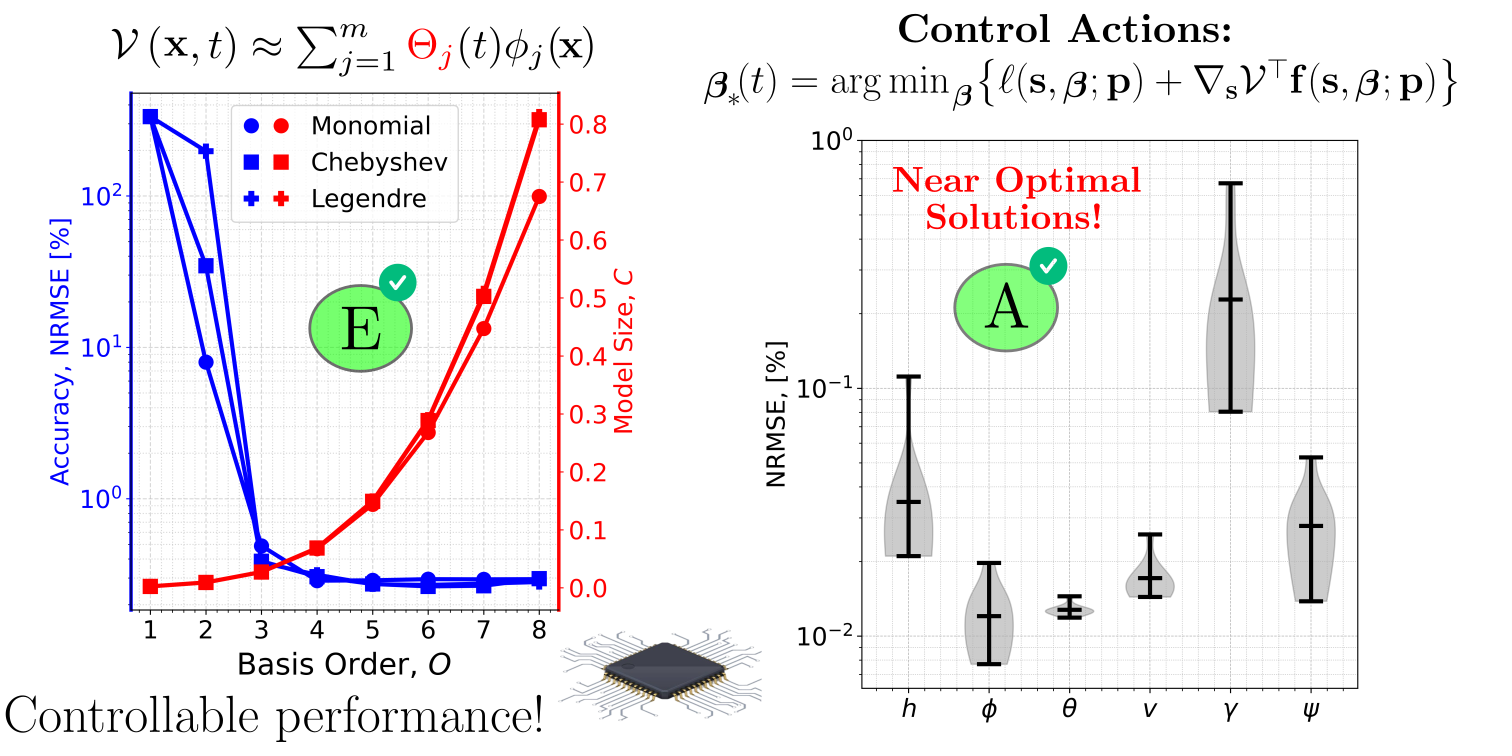
\includegraphics[width=0.9\textwidth]{../figs/sparsehjb/performance_ae_4.png}
        \end{figure}}
\end{frame}

\begin{frame}{\small Real-time control for the \textbf{space shuttle during re-entry} to maximize \textbf{cross-range},}
    \footnotesize
    \begin{columns}
        \begin{column}{0.7\textwidth}
            \only<2>{
                \begin{figure}
                    \centering
                    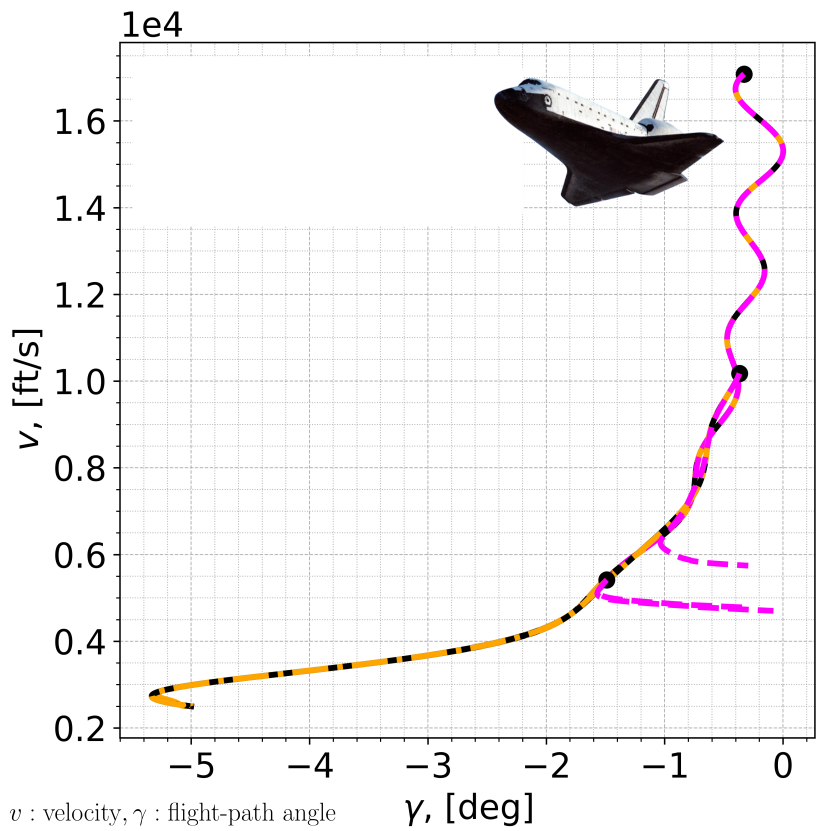
\includegraphics[width=0.65\textwidth]{../figs/sparsehjb/performance_ss_1.png}
                \end{figure}}
            \only<3>{
                \begin{figure}
                    \centering
                    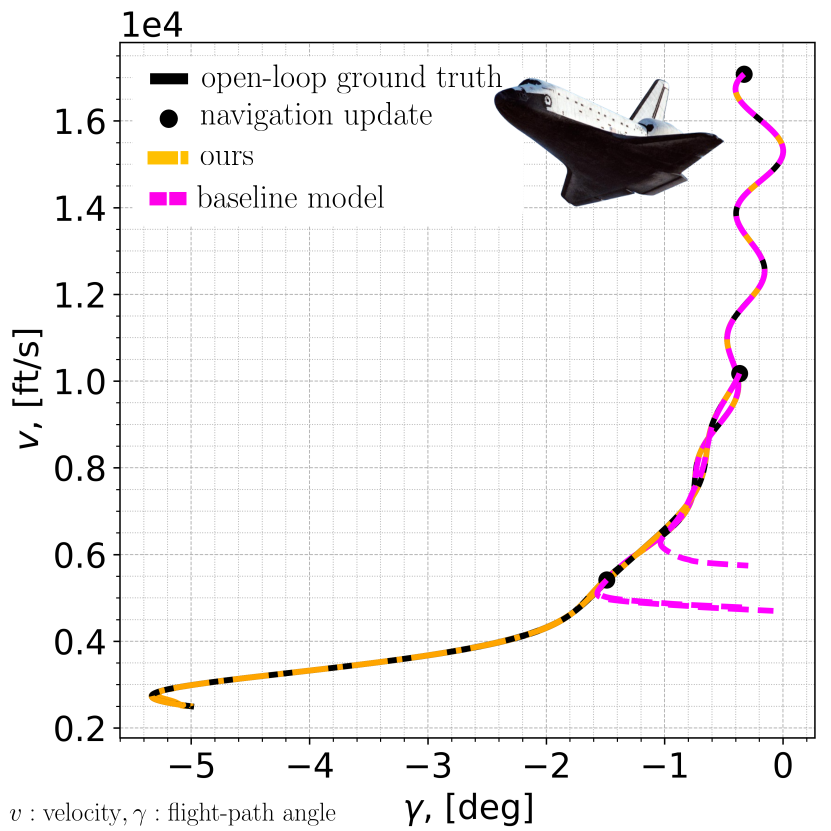
\includegraphics[width=0.65\textwidth]{../figs/sparsehjb/performance_ss_2.png}
                \end{figure}}
            \only<4>{
                \begin{figure}
                    \centering
                    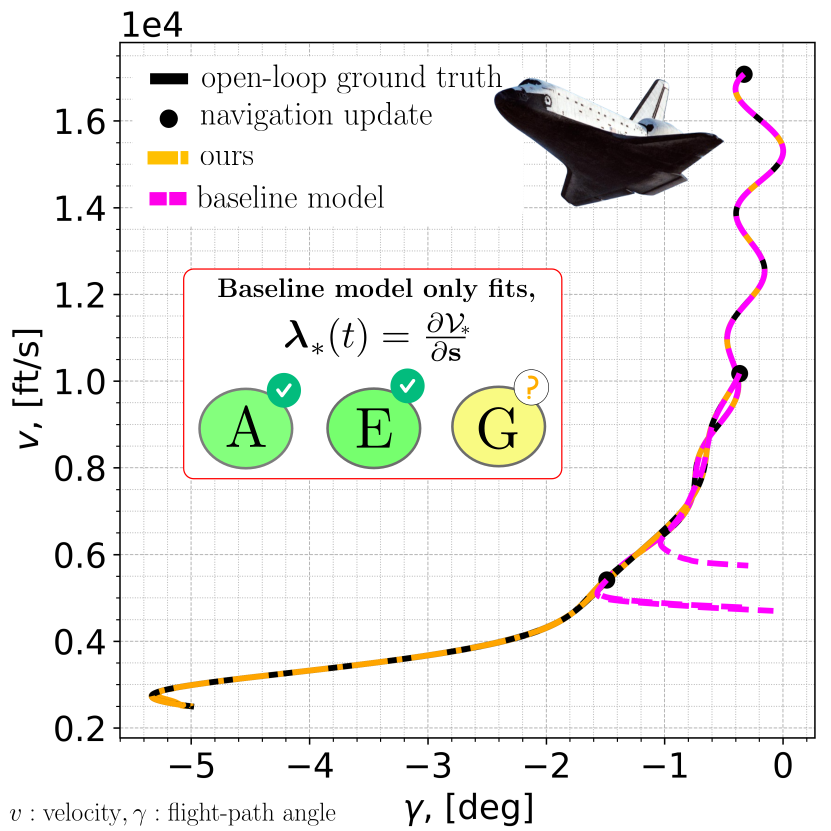
\includegraphics[width=0.65\textwidth]{../figs/sparsehjb/performance_ss_3.png}
                \end{figure}}
            \only<5->{
                \begin{figure}
                    \centering
                    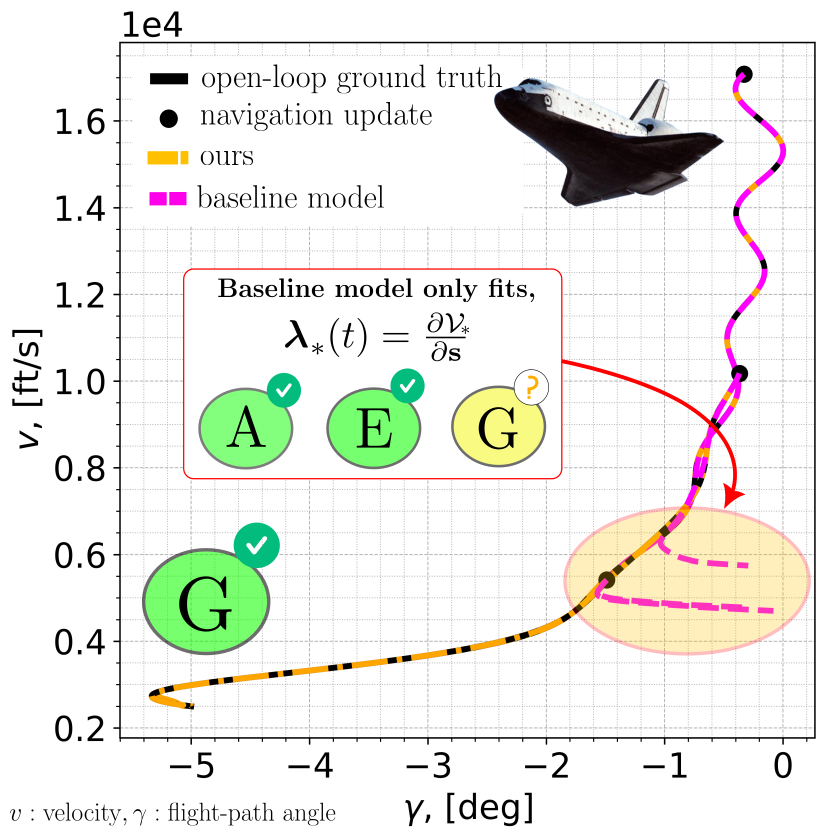
\includegraphics[width=0.65\textwidth]{../figs/sparsehjb/performance_ss_4.png}
                \end{figure}}
        \end{column}
        \hspace*{-1in}
        \begin{column}{0.4\textwidth}
            \visible<6->{
            \begin{graybox}{Key Results}
                \begin{itemize}
                    \item Improved \textbf{generalizability},
                    \item \textbf{Accelerations} $\approx10^4$,
                    \item \textbf{Model compressions} $\approx30\%$
                \end{itemize}
            \end{graybox}}
        \end{column}
    \end{columns}
\end{frame}

\begin{frame}{\small Is the Impossible Trinity of Optimal Control \textbf{solved}?}
    \footnotesize
    \begin{columns}
        \begin{column}{0.4\textwidth}
            \centering
            \visible<2->{
            \begin{figure}
                \centering
                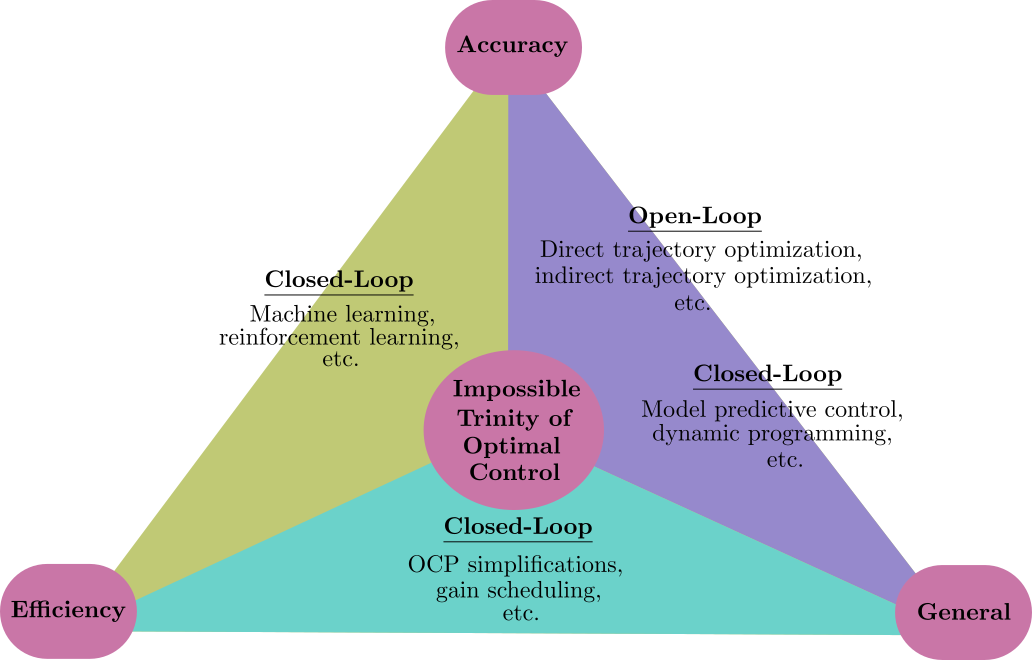
\includegraphics[width=0.9\textwidth]{../figs/introduction/itoc.png}
            \end{figure}}
        \end{column}
        \begin{column}{0.7\textwidth}
            \centering
            \begin{itemize}
                \item<3-> \textbf{Accuracy}: comparable to indirect OCP solutions (NRMSE $<1\%$)
                \item<4-> \colorbox{green!30}{\textbf{Efficiency}}:
                \begin{itemize}
                    \item<5-> \colorbox{green!30}{\textbf{Accelerations} $\approx 10^3 - 10^4$}
                    \item<6-> \colorbox{green!30}{\textbf{Model compressions} $\approx 80\%$}
                \end{itemize}
                \item<7-> \colorbox{green!30}{\textbf{Generalizability}: unseen BCs and model parameters}, but no guarantees outside the tube!
                \item<8-> Offline training costs \colorbox{red!30}{not quantified (future work)}
            \end{itemize}
        \end{column}
    \end{columns}
    \visible<3->{
    \begin{tikzpicture}[remember picture, overlay]
        \node[anchor=north west, xshift=2.2cm, yshift=-2.2cm] at (current page.north west) {
\includegraphics[width=0.1\textwidth]{../figs/pirom/checkmark.png}};
    \end{tikzpicture}}
    \visible<4->{
    \begin{tikzpicture}[remember picture, overlay]
        \node[anchor=north west, xshift=0.07cm, yshift=-5.0cm] at (current page.north west) {
\includegraphics[width=0.1\textwidth]{../figs/pirom/checkmark.png}};
    \end{tikzpicture}}
    \visible<7->{
    \begin{tikzpicture}[remember picture, overlay]
        \node[anchor=north west, xshift=4.45cm, yshift=-5.0cm] at (current page.north west) {
\includegraphics[width=0.1\textwidth]{../figs/pirom/checkmark.png}};
    \end{tikzpicture}}
\end{frame}


